\PassOptionsToPackage{dvipsnames}{xcolor}
\documentclass[submission, PhysCore]{SciPost}
\pdfoutput=1 % force pdfLaTeX on arXiv (pgfplots + PNG raster fields require it)

% SciPost template (SciPost.cls 2021-08, the class version with the PhysCore option): fonts and link colours.
% The template's \binoppenalty=\relpenalty=10000 (no line breaks in inline math) is not used: with this paper's
% inline formulas it pushed lines up to 100 pt into the margin.
\hypersetup{
    colorlinks,
    linkcolor={red!50!black},
    citecolor={blue!50!black},
    urlcolor={blue!80!black}
}
\usepackage[bitstream-charter]{mathdesign}
\urlstyle{sf}
\DeclareSymbolFont{usualmathcal}{OMS}{cmsy}{m}{n}
\DeclareSymbolFontAlphabet{\mathcal}{usualmathcal}

\usepackage{amsthm}
\usepackage{booktabs}
\usepackage{array}
\usepackage{adjustbox}
\usepackage{dsfont}
\newcommand{\openone}{\mathds{1}}% identity operator (revtex's \openone)
\usepackage{bm}
\usepackage{pgfplots}
\pgfplotsset{compat=1.18}
\usetikzlibrary{arrows.meta,positioning,calc,decorations.pathreplacing,decorations.markings,fit,backgrounds}
\usepgfplotslibrary{groupplots,fillbetween}
% figstyle.tex -- shared visual identity for all native pgfplots/TikZ figures.
% One palette, one colormap, one axis style so every figure reads as one system.
% Locked Paper-2 palette (replaces the drifted matplotlib values).

\definecolor{pIndigo}{HTML}{233047}   % structure / estimator-neutral
\definecolor{pAmber}{HTML}{D98E32}    % fires (fill / marker face)
\definecolor{pTeal}{HTML}{1B998B}     % corroborate / agree ONLY
\definecolor{pOx}{HTML}{8C2F2A}       % fires (line / marker edge)
\definecolor{pCrimson}{HTML}{C0392B}  % threshold
\definecolor{pInk}{HTML}{1B1B1B}
\definecolor{pMuted}{HTML}{7A7A7A}
\definecolor{pBlind}{HTML}{7A7A7A}    % blind = grey everywhere
\definecolor{pGrid}{HTML}{ECEAE5}
\definecolor{pCream}{HTML}{F4E9D8}

% paperhot: perceptual warm sequential, true-black foot so spectral gaps render black.
% 6 stops ported EXACTLY (equally spaced, raw sRGB) so a rasterized PNG field and the
% native pgfplots colorbar agree.
\pgfplotsset{
  colormap={paperhot}{
    rgb255=(22,8,5)
    rgb255=(90,22,11)
    rgb255=(176,54,12)
    rgb255=(217,142,50)
    rgb255=(246,196,83)
    rgb255=(251,239,199)
  }
}

% Base axis style: outside ticks, ink lines, legible fonts (>= ~2mm), light grid on top.
\pgfplotsset{
  paperaxis/.style={
    tick align=outside,
    tick style={pInk, line width=0.6pt},
    axis line style={pInk, line width=0.9pt},
    every axis label/.style={font=\normalsize, color=pInk},
    tick label style={font=\small},
    title style={font=\normalsize, color=pInk},
    label style={font=\normalsize},
    grid=major,
    grid style={pGrid, line width=0.5pt},
    axis on top,
    enlargelimits=false,
  },
}

% Reusable semantic styles -- encode the ONE identity across figures.
\pgfplotsset{
  firesline/.style ={pOx, very thick, mark=*, mark options={fill=pAmber, draw=pOx, line width=0.6pt}},
  firesband/.style ={pAmber, fill opacity=0.30},
  blindline/.style ={pBlind, thick, dashed, mark=square*, mark options={fill=white, draw=pBlind}},
  agreeline/.style ={pTeal, very thick},
  threshold/.style ={pCrimson, dash pattern=on 3.2pt off 2.4pt, line width=0.8pt},
  guide/.style     ={pInk, densely dashed, line width=0.7pt},
  halo/.style      ={white, line width=3pt},
}

% TikZ node styles for schematic figures (hero, insets).
\tikzset{
  pbox/.style   ={rounded corners=3pt, draw=pInk, line width=0.8pt, inner sep=6pt, align=center, font=\small},
  pflow/.style  ={-{Stealth[length=3.2mm]}, pInk, line width=1.0pt},
  pforbid/.style={-{Stealth[length=3.2mm]}, pMuted, line width=0.9pt, densely dashed},
  guide/.style  ={pInk, densely dashed, line width=0.7pt},
  halo/.style   ={white, line width=3pt},
}


\newtheorem{theorem}{Theorem}
\newtheorem{proposition}{Proposition}

% Figures drawn for a single APS column (width=\columnwidth) keep their proportions in the one-column layout.
\newcommand{\onecolfig}{\setlength{\columnwidth}{0.65\textwidth}}

\setlength{\emergencystretch}{2.5em}% absorb residual inline-math overfulls into invisible micro-stretch

\begin{document}

\begin{center}{\Large \textbf{
Reconstruction-independent moment tests for quantum-computed dynamical spectra
}}\end{center}

\begin{center}
Nicol\'as Bonilla Vargas\textsuperscript{1,2,3$\star$}
\end{center}

\begin{center}
{\bf 1} Universidad Nacional de Colombia, Bogot\'a, Colombia
\\
{\bf 2} SRH University, Munich, Germany
\\
{\bf 3} Daita AI, Munich, Germany
\\
${}^\star$ {\small \sf ngbonillav@unal.edu.co}
\end{center}

\begin{center}
\today
\end{center}

% Line numbers for refereeing (SciPost template option).
\linenumbers
% Affiliations aligned with the companion (arXiv:2608.16436v3, main.tex:231-235). Daita AI is a
% company: its role is stated under "Competing interests" in the back matter (author decision, 2026-09-27).

\section*{Abstract}
{\bf
Sample-based quantum diagonalization now reconstructs dynamical spectral functions $A(\omega)$ classically in subspaces sampled on a quantum processor. We develop and calibrate a screen comparing the moments read off a reconstruction with ground-state operator expectations that never use $A(\omega)$. A mismatch beyond a preset threshold rejects it; a pass does not certify it. In a hash-sealed, blinded simulation of 300 doped Hubbard-ring instances, the pre-registered primary endpoint was a detection rate of 53.7\% (101/188; Wilson 95\% CI 46.6--60.7\%) at a false-positive rate of 0.9\% (1/112), with an unbiased simulated estimator. The screen caught all 56 determinant truncations, 74\% of spurious features and none of 71 under-converged Krylov reconstructions; two sealed secondary predictions failed. Classical moment brackets state what a pass implies; at the deployed order ($m_0$--$m_2$) guaranteed power against fixed-pole redistributions is zero. On IBM Heron only the sampled support comes from the device. The missed weight $\Delta_0$ grows from 0.004 to 0.37 as coverage falls from 94\% to 35\%, but it rewards support spreading: a uniform in-sector sampler reaches lower $\Delta_0$, and the reconstruction with $\Delta_0=0.004$ has a relative $L_1$ error of 0.35. The discriminating moments $m_1,m_2$ remain simulation-only; a sealed noise gate for an on-device momentum-distribution test failed.
}

\vspace{10pt}
\noindent\rule{\textwidth}{1pt}
\tableofcontents\thispagestyle{fancy}
\noindent\rule{\textwidth}{1pt}
\vspace{10pt}

\begin{figure}[t]
\centering
\adjustbox{max width=\textwidth}{% fig_hero.tex -- the reconstruction-independent moment loop, native TikZ (no PNG).
% 2026-09-27 revision: outcome boxes read "reject: Delta_k > tau_k" / "pass: Delta_k <= tau_k" (tau_k = z delta_k,
% the preset threshold of the Method; a pass is not a certificate). The strapline states the one-sample-set DESIGN;
% in this paper both branches share shots only in simulation, and on hardware the device supplies the support S alone
% (caption). The footer prints the double-commutator form O_k = J ad_H^k(J), which the caption identifies as the
% exact-eigenstate form of the deployed estimator <J (H-e0)^k J>.
\begin{tikzpicture}[font=\small]
  % --- nodes ---
  \node[pbox, fill=pGrid!40, minimum height=10mm] (S)
      at (0.8,2.2) {computational-basis\\ samples $\mathcal{S}$};
  \node[pbox, draw=pInk, fill=white, minimum height=10mm] (REC)
      at (5.2,3.5) {reconstruction\\ $A(\omega)$};
  \node[pbox, draw=pIndigo, fill=pIndigo!8, minimum height=10mm] (MOM)
      at (5.2,0.9) {independent moments\\ $\widehat m_k=\langle O_k\rangle$};
  \node[pbox, draw=pInk, fill=white, minimum height=10mm] (CMP)
      at (9.9,2.2) {compare\\ $\Delta_k=\lvert\widehat m_k-\bar m_k\rvert$};
  \node[pbox, draw=pTeal, fill=pTeal!10, minimum height=9mm] (CORR)
      at (14.3,3.4) {\textbf{pass}\\ $\Delta_k\le\tau_k$\\[-1pt] {\scriptsize\itshape (not a certificate)}};
  \node[pbox, draw=pOx, fill=pOx!8, minimum height=9mm] (FALS)
      at (14.3,1.0) {\textbf{reject}\\ $\Delta_k>\tau_k$};

  % --- flow arrows ---
  \draw[pflow] (S) to[out=60,in=180]  (REC.west);
  \draw[pflow] (S) to[out=-60,in=180] (MOM.west);
  \draw[pflow] (REC.east) to[out=0,in=120]  (CMP.north west);
  \draw[pflow] (MOM.east) to[out=0,in=-120] (CMP.south west);
  \draw[pflow] (CMP.east) to[out=60,in=180]  (CORR.west);
  \draw[pflow] (CMP.east) to[out=-60,in=180] (FALS.west);

  % --- forbidden path: A(w) is NEVER read back into the moment branch ---
  \draw[pforbid] (REC.south) -- (MOM.north)
      node[midway] (X) {};
  \node[circle, draw=pOx, line width=0.9pt, minimum size=4.2mm, inner sep=0pt] at (X) {};
  \draw[pOx, line width=0.9pt] ($(X)+(-0.15,-0.15)$) -- ($(X)+(0.15,0.15)$);
  \node[font=\scriptsize\itshape, pMuted, align=center, anchor=east] at ($(X)+(-0.45,0)$)
      {never read\\ back off $A(\omega)$};

  % --- strapline + footer ---
  \node[font=\normalsize\bfseries, pInk, anchor=west] (STRAP) at (0.4,4.55)
      {Two moment branches from one sample set (design)};
  \node[font=\scriptsize\itshape, pMuted, anchor=base west] at ($(STRAP.base east)+(0.15,0)$)
      {shared shots realized in simulation only};
  \node[font=\scriptsize, pMuted, anchor=west] at (0.4,-0.15)
      {$O_k=J\,\mathrm{ad}_H^{k}(J)$, \; $m_0=\langle J^2\rangle$, \; $m_1=\tfrac12\langle[J,[H,J]]\rangle$ \;\textemdash\; the estimator never uses $A(\omega)$, so agreement is not preordained};
\end{tikzpicture}
}
\caption{\textbf{Two moment branches from one sample set (design).} Computational-basis samples fix a subspace $\mathcal S$. The reconstruction branch diagonalizes $H$ in $\mathcal S$, assembles $A(\omega)$ and reads off $\bar m_k=\int\omega^k A(\omega)\,d\omega$. The estimator branch evaluates the ground-state operator moment $\widehat m_k=\langle J(H-e_0)^kJ\rangle$ with $e_0=\langle H\rangle$ on the prepared state; on an exact eigenstate this equals $\langle J\,\mathrm{ad}_H^{k}(J)\rangle$, the form printed in the drawing (Appendix~\ref{app:moments}). It never uses $A(\omega)$, so it can disagree with the reconstruction. The reconstruction is rejected when $\Delta_k=|\widehat m_k-\bar m_k|$ exceeds a threshold $\tau_k=z\,\delta_k$ fixed in advance from shot noise and a bias budget; a pass does not certify it. In this paper the two branches share one set of shots only in simulation; on hardware the device supplies the support $\mathcal S$ alone (Sec.~\ref{sec:device}).}
\label{fig:hero}
\end{figure}

\section{Introduction}
Dynamical response functions connect many-body theory to experiment. The single-particle spectral function $A(k,\omega)$ is measured by angle-resolved photoemission~\cite{Damascelli2003}, the dynamical structure factors $S(q,\omega)$ and $S^{zz}(q,\omega)$ by inelastic neutron and resonant x-ray scattering, and the optical conductivity by infrared spectroscopy~\cite{Basov2011,Benthien2004,Qin2022}. Quantum processors, first used for static ground-state energies~\cite{AspuruGuzik2005,Peruzzo2014,McArdle2020,Bauer2020,Bravyi2022}, now return such functions as well. Trapped-ion devices have produced dynamical structure factors and single-particle spectral functions~\cite{GranetDSF2026,GranetARPES2026}, and Green's functions built from measured Hamiltonian moments~\cite{GreeneDiniz2024}. On superconducting processors, a DFT+DMFT workflow has computed its impurity Green's function with up to 14 qubits~\cite{Selisko2025}, and structure factors computed with up to 50 qubits have been compared quantitatively with neutron-scattering data~\cite{Lee2026}. Sample-based diagonalization and quantum Krylov methods, developed for ground states~\cite{QSCI2023,SQDchem2025,SKQD2501,Yoshioka2025,Motta2020}, have been extended to spectra~\cite{SQDspec2608,Patel2026}. In this quantum-centric pattern the device samples a subspace, and classical resources diagonalize the Hamiltonian in it and assemble $A(\omega)$~\cite{Alexeev2024}. The hardware run of our companion study is exact by coverage and establishes only that this pipeline executes; its post-selection read the bitstrings in reversed bit order, so all of its retained determinants came from device errors~\cite{SQDspec2608}.

Such results matter most where no trusted classical cross-check exists, which is the regime that motivates the quantum resource. The edge of that regime moves as classical methods improve and earlier demonstrations are dequantized~\cite{Preskill2018,Daley2022,Kim2023,Tindall2024,Tang2019,Hangleiter2023}; for sample-based diagonalization it is surveyed in Ref.~\cite{BonillaReviewSQD2026}. That regime is the eventual target, not the setting of this paper. A check intended for it must first be specified and calibrated where the ground truth is known~\cite{Eisert2020,Carrasco2021,Elben2020,Lubinski2023,Flammia2011}, and that is what we do here. Physics supplies the conditions. Every $T=0$ Lehmann spectrum must satisfy moment sum rules~\cite{HohenbergMartin1965,Kohn1964,Maldague1977} and positivity~\cite{Lehmann1954}, and the state behind it must satisfy its conserved-charge identities~\cite{Gauss2020}, however it was computed.

Current practice validates a quantum-computed spectrum against a reference. Lee \emph{et al.}\ compare with neutron data~\cite{Lee2026}. Buchs \emph{et al.}\ build a validation framework with experimental and classical anchors, whose metrics include windowed weights, low-order moments and sum-rule residuals~\cite{Buchs2026}; for the regime without full classical benchmarks they outline an asymmetric mode that would lean more on experiment, sum rules and internal consistency, and leave it to future work. Other verification tools certify a number rather than a function. Self-verifying variational simulation~\cite{Kokail2019} prepares a state variationally~\cite{Peruzzo2014,Cerezo2021,Bharti2022} and bounds its distance to an eigenstate through a measured energy variance. State certification from single-qubit measurements~\cite{HuangPreskillSoleimanifar2024}, error mitigation~\cite{TemmeBravyi2017,Kandala2019,EndoBenjaminLi2018,vandenBerg2023,Cai2023}, randomized-measurement estimation~\cite{HuangKuengPreskill2020,Elben2023}, observable estimation without classical verification~\cite{OEACV2026}, and bounded-error analog simulation from learned Hamiltonians and Lindbladians~\cite{Kraft2026} all act on states or expectation values. None of them checks a reconstructed $A(\omega)$ against the Hamiltonian that produced it without a classical or experimental reference. The failure we target is spectral weight placed at the wrong frequencies while integrated quantities stay within tolerance. Critical studies of quantum-selected configuration interaction and subspace diagonalization document the limitations of these methods for ground-state energies~\cite{Reinholdt2025,Epperly2022,Kirby2024,GaberleJattana2026,VaqueroSabater2026}; that the same mechanisms misassign spectral weight is our extrapolation. The same concern motivates response-targeted determinant selection on the classical side~\cite{LRSCI2025}. Figure~\ref{fig:akw} illustrates the target with an injected example: a corrupted $A(k,\omega)$ that passes visual inspection and a total-weight check but carries the wrong first moment.

The screen compares two sets of moments of the spectral measure (Fig.~\ref{fig:hero}). For a zero-temperature Lehmann function of a probe $J$, the moments $m_k=\int\omega^kA(\omega)\,d\omega$ are ground-state expectations, $m_0=\langle J^2\rangle$, $m_1=\tfrac12\langle[J,[H,J]]\rangle$ and in general $m_k=\langle J(H-E_0)^kJ\rangle$; they follow from operator algebra, not from the dynamics~\cite{Lehmann1954,Kubo1957,HohenbergMartin1965}. The reconstruction supplies its own moments $\bar m_k$. The estimate $\widehat m_k$ of the ground-state expectation is never obtained by integrating $A(\omega)$, so it can disagree with the reconstruction; a moment read back off $A(\omega)$ cannot, since compared with itself it gives $\Delta_k\equiv0$. The reconstruction is rejected when $\Delta_k=|\widehat m_k-\bar m_k|$ exceeds a threshold $\tau_k$ fixed in advance from shot noise and a bias budget. These are necessary conditions: failing one rejects the reconstruction at the pre-registered level, while passing does not show that the reconstruction is correct; it rules out only errors that move a tested moment past its threshold. The battery also accepts any exactly known operator identity; Appendix~\ref{app:gauss} uses the U(1) Gauss law as a state-level example, estimable from computational-basis samples in principle and here evaluated exactly on the state vector~\cite{Gauss2020,Kokail2019}.

The design takes both branches from one set of samples; Sec.~\ref{sec:role} states how far this is realized (not on hardware, where the device supplies only the sampled support; only in part, in simulation; and not in the blinded test).

Checking a computed spectrum against its moments is long-standing. In dynamical mean-field theory and quantum Monte Carlo, low-order moments of Green's functions and self-energies serve as consistency tests of continued spectra, most systematically in the sum-rule program of Turkowski and Freericks~\cite{TurkowskiFreericks2006,Freericks2009}, and analytic-continuation pipelines report sum-rule agreement routinely~\cite{Jarrell1996,Sandvik1998}. We claim no novelty for testing a spectrum against sum rules. In the optical case $m_0=\langle J^2\rangle$ is the total current--current weight, while the $f$-sum rule $\int_0^\infty\sigma_1\,d\omega=\tfrac{\pi}{2}\langle-\hat T\rangle$ is the separate moment $m_{-1}$~\cite{Kohn1964,Maldague1977,Basov2011}. Which moment sequences a positive measure can carry, and how tightly finitely many moments constrain it, is the classical moment problem~\cite{ShohatTamarkin1943,Akhiezer1965,KreinNudelman1977,Simon1998}. Its link to orthogonal polynomials and Gauss quadrature~\cite{GM2010,Szego1975,GolubWelsch1969,Nevai1986,Lanczos1950} also underlies the kernel-polynomial and recursion methods~\cite{KPM2006,Haydock1972,Silver1996,Holzner2011}. The same machinery now gives rigorous bounds on smeared spectral functions from Euclidean lattice correlators~\cite{AbbottJayOare2025,CausalBootstrap2026,CertifiedSpectral2026}; our moments come instead from ground-state operators, and our use is a rejection test on a real-frequency reconstruction. The semidefinite certificates of Wang \emph{et al.}\ and Mortimer \emph{et al.}\ return two-sided intervals on ground-state expectations, the latter at finite measurement statistics~\cite{WangAcin2024,Mortimer2026}. Requiring the read-off moments $\bar m_k$ to lie in such intervals is a second necessary condition on the reconstruction. Combining the two layers therefore gives two necessary conditions, at least as sharp as either alone, not a necessary condition paired with a sufficient one. We have not applied those programs to our moment operators; Sec.~\ref{sec:stack} shows the two layers side by side at the exact-moment level only, with a classical interval (Hausdorff) condition in place of the semidefinite program. Finally, some pipelines conserve the zeroth moment by construction. The Green's-function solver of Patel \emph{et al.}\ augments its response subspace so that the probe acting on the sampled ground state is held exactly, and the spectral weight is then never lost~\cite{Patel2026}. When both branches use the same ground-state vector, our coverage channel carries no signal for such pipelines; only the higher moments test them.

This paper is the methodological complement of a companion study that reconstructs these spectra from sampled subspaces and bounds their error~\cite{SQDspec2608}. Version~3 of the companion contains results that this screen uses, and we adopt its terms. The operator leak of Eq.~\eqref{eq:app-leak}, with $|\varphi\rangle=J|0\rangle$, contains two of them. At $k=0$ it is the coverage residual $\Delta_0=m_0(1-w)$, with $w$ the companion's captured weight. At $k=2$, on a subspace of unit captured weight, it is the companion's identity $\mu_2-\mu_2^{\mathcal S}=\lVert Q_{\mathcal S}HP_{\mathcal S}\varphi\rVert^2$, where $\mu_j$ is the companion's name for $m_j$. The companion also proves that a subspace containing the order-$K$ Krylov space reproduces the moments through order $2K+1$. This is why Krylov reconstructions with two or more Lanczos nodes reproduce $m_0$--$m_2$ exactly and pass our battery, while the one-node case misses $m_2$ by $2$--$4\%$ and passes only inside the $2\%$ bias budget. Finally, the companion shows that the captured weight alone cannot certify a reconstruction, and our $L=8$ device run gives an instance on device data. What this paper adds is not an error bound. It is a rejection test with thresholds that include shot noise and a bias budget, applied to single-particle, current and collective response functions; a blinded, sealed calibration of its false-positive and detection rates; the exact limits of what a pass implies; and a device evaluation of the coverage channel against reference distributions. In detail:

\emph{(i) Screens across observables} (Figs.~\ref{fig:akw}--\ref{fig:collective_screen}). In the doped Hubbard current response a spurious low-frequency peak that preserves $m_0=\langle J^2\rangle$ is rejected by $m_1$, the mean frequency once normalized by $m_0$~\cite{Kohn1964,Maldague1977}. The negative-order moment $m_{-1}$ moves most in relative terms ($154\%$ against $38\%$ for $m_1$). Normalized by noise at a $2\%$ bias, however, it fires later than $m_1$ and $m_2$ for this error model, on the ring and on the open chain; among the peak positions we scanned it fires first only at $0.5\,t$ and below. On the ring it also needs the Kohn stiffness from a separate calculation. The same construction applies to $A(k,\omega)$ and to the collective $S(q,\omega)$ and $S^{zz}(q,\omega)$, each a positive $T=0$ Lehmann measure with its own sum rules; these are exact simulations at $L\le12$.

\emph{(ii) Independence under truncation} (Sec.~\ref{sec:teeth}). Under determinant-subspace truncation the independent estimator crosses its threshold while a control read back off $A(\omega)$ stays identically zero~\cite{SQDchem2025,QSCI2023}. The same holds when both branches are evaluated on one subspace state.

\emph{(iii) A blinded, pre-registered calibration} (Sec.~\ref{sec:blind}). Before any instance existed we sealed the battery, thresholds, error catalog and seed by a SHA-256 hash; the seal is self-attested, with no third-party timestamp. The sealed primary endpoint was a detection rate of $53.7\%$ ($101/188$, Wilson $95\%$ interval $[46.6,60.7]\%$) at a false-positive rate of $0.9\%$ ($1/112$, $[0.2,4.9]\%$). By class, the battery caught $56/56$ determinant truncations, $45/61$ spurious features and $0/71$ under-converged Krylov reconstructions; rescoring the 56 sealed truncations post hoc with the shared-state estimator also rejects all of them. The sealed secondary predictions held for truncations, for weight-changing spurious features ($25/27$ caught) and for Krylov reconstructions with two or more nodes ($0/56$ caught); two failed. The one-node Krylov case, expected to be caught, was caught in $0$ of $15$ instances. The weight-preserving spurious features, expected to be rarely caught, were caught in $20$ of $34$ ($59\%$), an outcome the pre-registration did not anticipate. The low false-positive rate is largely built in: the simulated estimator is unbiased while the threshold budgets a $2\%$ bias, and a realized bias of $+2\%$ ($-2\%$) would raise the modeled rate from $1.3\%$ to $8.0\%$ ($11.5\%$). The $0.9\%$ therefore confirms the implementation, not robustness to a real mitigation bias, which is untested. The positivity branch, applied to the reconstruction's own moments, cannot fire on a catalog of positive measures. The catalog is one doped $L=6$ ring at $U/t\in\{3,4,5,6\}$ with the current probe; its 56 truncation depths were drawn at random, and by ground-state weight the truncations are mild (they keep $75$--$99\%$ of it). An exhaustive scan of every depth for the $U/t=4$ member, with the interval battery of Appendix~\ref{app:estimator}, finds 12 of 185 depths at which the full battery, with the sealed thresholds, passes the truncated reconstruction, three of them (46--51\% of the support) inside the depth range of the catalog. The $56/56$ therefore describes the sealed draw, not every truncation.

\emph{(iv) Exact limits} (Secs.~\ref{sec:christoffel} and~\ref{sec:detect}). Classical Christoffel--Markov--Stieltjes and Markov--Krein brackets, re-derived here, bound how far the cumulative weight of a reconstruction with exact moments can deviate from the true one~\cite{GM2010,Totik2000}. At the deployed order the bracket is vacuous at the mean ($\max_tW_1=m_0$), and finite tolerances widen it further. On $N$ distinct poles the first $N$ moments are complete for fixed-pole weight redistributions (Theorem~\ref{thm:detect}), but in exact arithmetic only. At the deployed order ($m_0,m_1,m_2$) and $N>3$ the guaranteed power is zero: the redistributions that preserve these moments form an $(N-3)$-dimensional space, whatever the pole separation. On the $L=6$ current spectrum ($N=5$) an explicit redistribution that keeps $m_0,m_1,m_2$ exact moves $72\%$ of the weight and empties two of the five poles; one that moves $86\%$ keeps $m_0,m_1$ exact, shifts $m_2$ by exactly $\tau_2$ and passes. Closing this gap needs moments beyond $m_2$. For weight moved within a cluster of $s$ poles of diameter $D$, the shots needed to see it grow at least as $D^{-2(s-1)}$.

\emph{(v) A device evaluation of the coverage channel} (Sec.~\ref{sec:device}). On IBM Heron (\texttt{ibm\_fez}) we ran seven circuits for an $L=8$ electron-addition sector at four shot budgets ($5\times10^4$ to $4\times10^3$ shots per circuit) and kept the raw counts. The circuits prepare a computational-basis determinant and apply on-site $R_{zz}$ phases and number- and spin-conserving $R_{xx}R_{yy}$ hopping without Jordan--Wigner strings, so they sample the addition sector but are not the Hubbard propagator of the probe state; the sampler used measurement twirling, Pauli gate twirling and dynamical decoupling, and the counts were post-selected to the physical sector without configuration recovery or readout-error mitigation. The device supplies only the support $\mathcal S$. The missed weight $\Delta_0$ grows from $0.0044$ to $0.37$ as coverage falls from $94\%$ to $35\%$, but it measures support, not fidelity. At $5\times10^4$ shots per circuit the device value lies below all $2000$ noiseless multinomial replicas of the same circuits at the same raw shot count, and at $4\times10^3$ above all of them. A uniform sampler over the sector, drawing as many in-sector samples as the device retained, reaches a lower $\Delta_0$ and a more accurate reconstruction than the device at every budget. The device reconstruction with $\Delta_0=0.0044$ has a relative $L_1$ error of $0.35$; that is still better than all 80 noiseless replicas we reconstructed at the same budget, while at $4\times10^3$ shots the device reconstruction is worse than all 80. The discriminating moments $m_1,m_2$ were not measured on the device: at the companion's circuit depth ($292$ CZ) the forecast depolarizing bias of the bond-basis estimate of $m_1$ is $37$--$116\%$ of the signal (local to global depolarizing at a two-qubit error of $2.5\times10^{-3}$). A sealed simulated noise gate for an on-device momentum-distribution test failed at the relaxed noise floors of its single permitted amendment ($T_1=100\,\mu$s, $T_2=70\,\mu$s, two-qubit error parameter $3.5\times10^{-3}$), and that run was not made.

\begin{table}[t]
\caption{\textbf{Contribution relative to the closest prior art.} ``recon.-indep.'' states whether the check compares a reconstruction with something the reconstruction did not produce, and with what; ``same samples'' states whether that comparison quantity comes from the samples that produced the spectrum; ``---'' marks an axis that does not apply to the method's object. The semidefinite programs bound the true moments; requiring the read-off moments to lie inside their intervals is a second necessary condition, not a sufficient one (Sec.~\ref{sec:stack}). $^{a}$Designed; realized only in part, and only in simulation (Sec.~\ref{sec:role}); same-sample estimation, blinded pre-registration and on-device execution have not been realized together in one experiment. $^{b}$The device supplies the sampled support only; the discriminating moments $m_1,m_2$ are simulation-only (Table~\ref{tab:scope}). $^{c}$Blinded simulation with an oracle-centred estimator (Sec.~\ref{sec:blind}). $^{d}$The companion's $L=6$ device run covers the whole sector, so its bound is not exercised on device data.}
\label{tab:contribution}
\footnotesize
\begin{tabular}{p{0.24\textwidth}p{0.17\textwidth}>{\raggedright\arraybackslash}p{0.09\textwidth}>{\raggedright\arraybackslash}p{0.10\textwidth}>{\raggedright\arraybackslash}p{0.07\textwidth}p{0.16\textwidth}}
\toprule
method & recon.-indep. & same samples & on device & blinded & role \tabularnewline
\midrule
\raggedright Turkowski--Freericks sum-rule checks~\cite{TurkowskiFreericks2006,Freericks2009} & \raggedright yes (vs classical) & no & no & no & \raggedright consistency check \tabularnewline
\raggedright maxent / stochastic continuation~\cite{Jarrell1996,Sandvik1998} & \raggedright yes (vs classical) & no & no & no & \raggedright consistency check \tabularnewline
\raggedright Buchs \emph{et al.}\ validation framework~\cite{Buchs2026} & \raggedright yes (vs experiment, classical, sum-rule targets) & no & no & no & \raggedright validation metrics, incl.\ moments \tabularnewline
\raggedright Lee \emph{et al.}\ neutron benchmark~\cite{Lee2026} & \raggedright yes (vs experiment) & no & yes & no & \raggedright benchmark \tabularnewline
\raggedright Greene-Diniz \emph{et al.}\ cumulant Lanczos~\cite{GreeneDiniz2024} & \raggedright --- (moments build $G$) & --- & yes & no & \raggedright constructive \tabularnewline
\raggedright Wang--Ac\'in / Mortimer SDP~\cite{WangAcin2024,Mortimer2026} & \raggedright --- (bounds moments) & no & no & no & \raggedright two-sided moment bounds \tabularnewline
\raggedright Abbott \emph{et al.}\ / causal bootstrap~\cite{AbbottJayOare2025,CausalBootstrap2026,CertifiedSpectral2026} & \raggedright yes (Euclidean) & no & no & no & \raggedright two-sided bound \tabularnewline
\raggedright Kokail \emph{et al.}\ self-verification~\cite{Kokail2019} & \raggedright --- (certifies state) & --- & yes & no & \raggedright state verification \tabularnewline
\raggedright reference-free observable estimation~\cite{OEACV2026} & \raggedright --- (certifies number) & --- & yes & no & \raggedright validity \tabularnewline
\raggedright companion: captured weight and leakage~\cite{SQDspec2608} & \raggedright --- (bounds the error) & --- & no$^{d}$ & no & \raggedright a posteriori error bound \tabularnewline
\raggedright \textbf{this work} & \raggedright \textbf{yes} & \textbf{designed}$^{a}$ & \textbf{support only}$^{b}$ & \textbf{yes}$^{c}$ & \raggedright \textbf{necessary condition} \tabularnewline
\bottomrule
\end{tabular}
\end{table}

We state the scope at the outset. The method can reject a reconstruction but cannot certify one; its conditions are necessary, not sufficient. The moment screen targets determinant-subspace truncation and spurious features in sample-based-diagonalization (SQD/QSCI) spectra, that is, weight and subspace misassignment; the Gauss-law identity targets gauge-symmetry violation in the prepared state. The screen is out of scope for Krylov-convergence errors: a subspace containing the order-$K$ Krylov space reproduces the moments through order $2K+1$~\cite{SQDspec2608}, so an under-converged Krylov reconstruction passes the battery (Sec.~\ref{sec:blind}). Detecting that error class calls for a separate instrument, most naturally a Ritz-residual convergence check on the Krylov basis, which we leave to future work. Neither check is a general device-noise diagnostic, which remains the province of noise-model and observable-estimation validation~\cite{OEACV2026}. The screen tests integrated moments, not pointwise line shapes; its positivity structure is that of a diagonal $T=0$ Lehmann spectrum~\cite{Lehmann1954}; and every demonstration is at a classically reproducible size (Hubbard chains and rings with $L\le12$, a small lattice-Schwinger model, and a DMRG scalability check at $L=24$). On hardware, moments carry statistical and systematic error, so the exact-moment tests must be replaced by interval tests before they can be trusted there (Appendix~\ref{app:estimator}); Table~\ref{tab:scope} separates what is measured on hardware, what is simulated and what is deferred.

\section{Method: reconstruction-independent moment tests}
We formalize the screen in two steps: first the object it tests---a quantum-computed spectrum and the samples that produced it---and then the checks we attach to it.

\subsection{The quantum processor and the origin of the samples}
\label{sec:role}
The object the screen tests is the output of a sample-based-diagonalization pipeline, and what the screen can say depends on that pipeline. The pipeline and the $L=6$ device spectrum of Fig.~\ref{fig:heron} are those of the companion study~\cite{SQDspec2608}. This paper contributes the test described below, its blinded calibration in simulation, its exact limits, and one new $L=8$ \texttt{ibm\_fez} job that supplies a device-sampled support (Sec.~\ref{sec:device}). In sample-based diagonalization~\cite{SQDchem2025,QSCI2023,SKQD2501} the processor does not evaluate $A(\omega)$. It prepares a state, and each computational-basis shot returns one bitstring, a candidate Slater determinant. The distinct bitstrings that survive post-selection to the physical particle-number and spin sector form the subspace $\mathcal{S}$. The Hamiltonian is projected onto $\mathcal{S}$ and diagonalized classically, and the spectrum is assembled as the $T=0$ Lehmann sum $A(\omega)=\sum_n|\langle n|J|0\rangle|^2\,\delta_\eta\!\big(\omega-(E_n-E_0)\big)$ over the resulting eigenpairs, with $\delta_\eta$ a narrow broadening~\cite{Lehmann1954}. In the companion's formulation the prepared state is a Trotterized real-time evolution of the $(N{+}1)$-particle seed $c^{\dagger}_p|\psi_0\rangle$~\cite{Mikkelsen2024}. The device circuits actually run---the companion's $L=6$ job and our $L=8$ job---are different. Each of their seven circuits prepares a computational-basis $(N{+}1)$ determinant with $X$ gates and applies Trotter layers of on-site $R_{zz}$ and $R_{xx}R_{yy}$ hopping gates without Jordan--Wigner strings. They are therefore number- and $S_z$-conserving samplers of the addition sector, not the Hubbard propagator of the seed, as the companion's v3 discloses for its run~\cite{SQDspec2608}. Neither run used configuration recovery~\cite{BonillaReviewSQD2026}; both used plain post-selection. The companion's $L=6$ run read the bitstrings in reversed qubit order during post-selection, so every determinant it retained arose from a device error~\cite{SQDspec2608}. Our $L=8$ job ($5{\uparrow},4{\downarrow}$ determinant) uses the correct bit order and post-selects to $N=9$ with $N_\uparrow-N_\downarrow=1$. It ran on SamplerV2 with measurement twirling, Pauli gate twirling and dynamical decoupling; no readout-error mitigation was applied to the counts.

The intended role of the processor appears only at scale. The many-body sector grows exponentially with system size, so the configurations that carry the weight of the probe state $|\varphi\rangle=J|0\rangle$ cannot in general be enumerated classically. An ideal sampler of the targeted state would concentrate shots on them and fix $\mathcal{S}$ by measurement rather than by a classical selection heuristic~\cite{SQDchem2025}. We do not show that any device sampler does this better than a classical heuristic, and the companion claims no quantum advantage~\cite{SQDspec2608}. The circuits run here are not targeted at $\varphi$. For them, the coverage residual $\Delta_0$ of Sec.~\ref{sec:device} measures how much of $\varphi$'s weight lies outside the configurations the sampler happened to reach. At $L=8$ a uniformly random in-sector sampler, given the device's retained shot counts, leaves less of that weight uncovered than the device does at every shot budget (Sec.~\ref{sec:device}).

The design goal is that the moment estimator and the reconstruction share the sampled support, so that $\widehat m_k$ inherits the shot noise and mitigation choices of the spectrum it tests. The independent estimator $\widehat m_k$ defined below applies the full operator to the subspace ground state built on $\mathcal{S}$. This is a classical post-processing step that reaches configurations outside $\mathcal{S}$ (Appendix~\ref{app:estimator}). A device-native alternative measures $\langle O_k\rangle$ on a separately prepared ground state in qubit-wise-commuting Pauli groups; it is simulated only (Appendix~\ref{app:estimator}). We state where the shared-sample design is realized. On hardware it is not: the device supplies only the support $\mathcal{S}$, and every moment in Sec.~\ref{sec:device} is computed classically. In simulation it is realized in three places: the shared-state test of Fig.~\ref{fig:teethshared}, where both moments are evaluated on one subspace state (there the subspace is a deterministic truncation by $|\psi_0|^2$, not a set of shots); the joint-sampling simulations of Sec.~\ref{sec:limits}, where one set of shots yields both $\widehat m_1$ and $\bar m_1$ (correlation $\rho\approx0.43$ at $84\%$ coverage and no gain in detection power; their local estimator uses exact amplitudes, so it is not device-realizable); and the $L=24$ DMRG test of Sec.~\ref{sec:limits}, where both branches use one sampled subspace. The blinded test of Sec.~\ref{sec:blind} does not use it: there $\widehat m_k$ is the exact moment plus Gaussian shot noise. Section~\ref{sec:blind} also reports a post hoc rescoring of its $56$ truncations with the shared-state estimator.

\subsection{The independent moment estimator and the falsifier}
A quantum-computed dynamical spectrum is thus delivered as a non-negative function $A(\omega)$ together with the sample set $\mathcal{S}$. For a zero-temperature diagonal Lehmann spectral function of an operator $J$, $A(\omega) = \sum_n |\langle n | J | 0\rangle|^2\,\delta(\omega - (E_n - E_0))$ is a positive measure on the real line. On an exact eigenstate its power moments $m_k = \int \omega^k A(\omega)\,d\omega$ are ground-state expectation values, $m_k=\langle 0|J(H-E_0)^kJ|0\rangle=\langle 0|J\,\mathrm{ad}_H^{k}(J)|0\rangle$, so that $m_0 = \langle J^2\rangle$ and $m_1 = \tfrac{1}{2}\langle [J,[H,J]]\rangle$ (Appendix~\ref{app:moments})~\cite{Lehmann1954,HohenbergMartin1965}. In the optical case $m_0$ is the total integrated current--current weight and $m_1/m_0$ the mean frequency, while the optical $f$-sum is the separate moment $m_{-1}$~\cite{Kohn1964,Maldague1977}. These operator forms coincide only on an exact eigenstate. On a subspace state they differ, by enough to change a verdict. For the current probe of the doped $L=6$, $U/t=4$ ring, truncated to the top $100$ of its $225$ sector configurations by $|\psi_0|^2$ ($44\%$ coverage), $\langle J(H-e_0)J\rangle=4.56$ while $\tfrac12\langle[J,[H,J]]\rangle=3.72$, against a reconstruction moment $\bar m_1=3.74$ and an exact $m_1=4.23$. At the deployed threshold $\tau_1=0.229$ (defined below) the first form rejects, as the exact moment would, and the second does not. The cut falls inside a $24$-fold degenerate $|\psi_0|^2$ shell, so these values depend on how ties are broken; the verdicts are the same in both tie orders we computed. We therefore fix the deployed estimator as $\widehat m_k=\langle J^\dagger(H-e_0)^kJ\rangle$ with $e_0=\langle H\rangle$ on the prepared state, the form used in the shared-state tests below.

The screen attaches to the spectrum an estimator $\widehat{m}_k$ of each moment that is independent of the reconstruction: it is never obtained by integrating $\omega^k A(\omega)$. We denote by $\bar{m}_k = \int \omega^k A(\omega)\,d\omega$ the reconstruction moment, the quantity a circular check would use. The test statistic is the discrepancy $\Delta_k = |\widehat{m}_k - \bar{m}_k|$. The true spectrum gives $\Delta_k = 0$ up to estimator error, so the reconstruction is rejected when $\Delta_k>\tau_k$, with $\tau_k=z\,\delta_k$, $z=1.96$, and $\delta_k^2=\operatorname{Var}(O_k)/N_s+b_k^2$ the shot variance plus a bias budget $b_k$ (Appendix~\ref{app:estimator}); the deployed rule uses $N_s=5\times10^4$ and $b_k=0.02\,|\widehat m_k|$. A circular check compares $\bar{m}_k$ with itself, returns $\Delta_k \equiv 0$ and can never reject; Results~II shows this contrast on controlled truncation. At $k=0$ the discrepancy is the weight the support misses, $\Delta_0=\langle\varphi|(\openone-\Pi_\mathcal{S})|\varphi\rangle$, which in the companion's notation is $m_0(1-w)$ with $w$ the captured weight~\cite{SQDspec2608}. The companion also proves two results that bound what this test can see. A subspace containing the order-$K$ Krylov space of $\varphi$ reproduces the moments through order $2K{+}1$, so a Krylov-adequate reconstruction passes any moment test up to that order by construction. For a subspace of unit captured weight, $m_0$ and $m_1$ are reproduced exactly and the first moment that can fail is $m_2$, with deficit $\lVert Q_\mathcal{S}HP_\mathcal{S}\varphi\rVert^2$; this is Eq.~\eqref{eq:app-leak} at $k=2$ with $\Delta_0=0$. The companion further shows that captured weight alone cannot certify a reconstruction~\cite{SQDspec2608}. What the present paper adds is the use of these residuals as a test with fixed thresholds: its sealed blinded calibration in simulation (Sec.~\ref{sec:blind}), the shared-state estimator (Sec.~\ref{sec:teeth}), exact statements of what passing means (Secs.~\ref{sec:christoffel} and~\ref{sec:detect}), the moment test on the negative-order and collective channels (Results~I), and an analysis of the coverage residual on a device-sampled support (Sec.~\ref{sec:device}).

The screen is a battery, not a single test. It applies $\Delta_k$ for $k = 0,1,\dots,K$ (deployed: $K=2$) and, separately, checks that the estimated sequence $\{\widehat{m}_k\}$ is itself a moment sequence of a positive measure. That requires the Hankel matrix $H_n=[\widehat m_{i+j}]\succeq 0$ and, because a diagonal $T=0$ Lehmann measure is supported on $\omega=E_n-E_0\ge 0$, also the shifted Stieltjes matrix $H_n^{(1)}=[\widehat m_{i+j+1}]\succeq 0$~\cite{ShohatTamarkin1943,Akhiezer1965,KreinNudelman1977} (Fig.~\ref{fig:momentcone}). A violation rejects the estimate---device, mitigation or estimator---independently of $A(\omega)$. It cannot reject a non-negative reconstruction, whose own moments satisfy these conditions by construction; in the blinded test the branch was applied to $\bar m_k$ and could not fire (Sec.~\ref{sec:blind}). The battery also accepts any exactly known operator identity: a conserved charge $[H,G]=0$ with a known physical eigenvalue gives a constraint on the prepared state whose violation rejects that state, as in the gauge-theory example below~\cite{Gauss2020}. The construction transports across models and observables because it needs only (a) a positive spectral measure and (b) operators whose ground-state expectations can be estimated without the reconstruction~\cite{KPM2006,GM2010}.

\begin{figure}[t]
\centering\onecolfig
% fig_momentcone.tex -- NEW native pgfplots (single column). The moment-problem geometry: a moment
% SEQUENCE is itself falsifiable, with no reference to A(omega). Valid moment body on [-1,1] m1^2<=m2<=1.
\begin{tikzpicture}
\begin{axis}[
  paperaxis, width=\columnwidth, height=6.6cm,
  xmin=-1.12, xmax=1.12, ymin=-0.03, ymax=1.08,
  xlabel={first moment $m_1$}, ylabel={second moment $m_2$},
]
  % Hankel-positive body: m1^2 <= m2 <= 1
  \addplot[name path=para, domain=-1:1, samples=140, draw=pInk, thick] {x^2};
  \addplot[name path=top, draw=none, forget plot] coordinates {(-1,1) (1,1)};
  \addplot[pAmber, fill opacity=0.16, forget plot] fill between[of=para and top];

  % schematic shot-budget interval boxes, each labelled INSIDE
  \draw[pTeal, thick, fill=pTeal, fill opacity=0.10] (axis cs:0.14,0.58) rectangle (axis cs:0.52,0.78);
  \node[pTeal!60!black, font=\scriptsize] at (axis cs:0.33,0.68) {survives};
  \draw[pOx, thick, fill=pOx, fill opacity=0.10] (axis cs:0.50,0.04) rectangle (axis cs:0.86,0.22);
  \node[pOx, font=\scriptsize] at (axis cs:0.68,0.13) {falsified};

  % the real computed moment point (nearly rank-1: sits on the parabola)
  \addplot[only marks, mark=*, mark size=3pt, mark options={fill=pTeal, draw=white, line width=1pt}]
      table[x=m1,y=m2]{figs/momentcone_point.dat};

  % labels in verified-empty regions (never on the parabola / boxes / frame)
  \node[pInk, font=\small, align=center] at (axis cs:0.02,0.94) {valid $\{m_k\}$ on $[-1,1]$};
  \node[pTeal, font=\scriptsize, anchor=west, align=left] at (axis cs:-1.09,0.30)
      {computed\\ $(m_1,m_2)$};
  \draw[pTeal, line width=0.5pt] (axis cs:-0.71,0.315) -- (axis cs:-0.60,0.338);
  \node[pInk, font=\scriptsize, anchor=west] at (axis cs:-1.09,0.05)
      {rank-1: $m_2{=}m_1^2$};
\end{axis}
\end{tikzpicture}

\caption{\textbf{Hankel-positivity region in the $(m_1,m_2)$ plane.} For a normalized measure ($m_0=1$) with frequencies rescaled to $[-1,1]$, the moments must lie in the body $m_1^2\le m_2\le 1$. The lower edge $m_2=m_1^2$ is the Hankel (rank-one) boundary, reached by a single $\delta$; the upper edge $m_2=1$ is the interval (Hausdorff) localizing condition of the $[-1,1]$ support. The two boxes are schematic shot-budget intervals on an estimated moment vector. A box that lies wholly in the Hankel-negative region $m_2<m_1^2$ (oxblood, ``falsified'') rejects the estimate with no reference to $A(\omega)$; a box inside the body (teal, ``survives'') passes. The check acts on the estimate: a non-negative reconstruction always has its own moments inside the body. The teal dot is the exact $(m_1,m_2)$ of the doped $L=6$, $U/t=8$ Hubbard current measure. The rescaling maps onto $[-1,1]$ the full range of excitation energies of the Fock-space Hamiltonian, $[0.148,52.21]\,t$, which includes states of zero weight; the weighted support $[2.49,13.92]\,t$ maps to $[-0.91,-0.47]$. In these units the measure is narrow, and one pole carries $78\%$ of its weight, so the dot lies just above the rank-one edge~\cite{ShohatTamarkin1943,Akhiezer1965}.}
\label{fig:momentcone}
\end{figure}

\section{Results I: weight-misassignment errors across observables}
We first show the physical spectra on which the screen operates. Figure~\ref{fig:akw} shows the single-particle spectral function $A(k,\omega)$ of the half-filled Hubbard ring: lower and upper Hubbard bands separated by the Mott gap, with the dispersion of a one-dimensional correlated insulator~\cite{Hubbard1963,LiebWu1968,Dagotto1994,Benthien2004,Preuss1995}. A truncated or otherwise corrupted reconstruction misplaces spectral weight. To illustrate what the first-moment check measures, we inject a corruption that flattens the band-centroid dispersion by moving weight between the Hubbard bands at each momentum, leaving the Mott gap and the per-$k$ total weight intact. It is the single-particle analogue of the optical weight misplacement of Fig.~\ref{fig:invfalsifier} and of the truncation errors of Fig.~\ref{fig:teeth}. The first moment at each momentum, given by the anticommutator sum rule for the non-Hermitian probe $c_{k\sigma}$ (Appendix~\ref{app:moments}), exposes the flattening (right panel). The corruption is built to move the centroid by a fixed fraction of $\epsilon_k$, and the moment is evaluated in closed form, so the residual is set by construction: the panel illustrates the check rather than testing it. The same construction applies to collective response. Figure~\ref{fig:sqw} shows the charge dynamical structure factor $S(q,\omega)$, gapped by a particle--hole excitation onset $\Delta_c$, and the spin structure factor $S^{zz}(q,\omega)$, whose gapless low-energy weight is the spinon continuum of the gapless spin sector~\cite{Voit1995}, a signature of spin--charge separation~\cite{Benthien2004}. Each channel is a positive $T=0$ Lehmann measure with its own moment sum rules, so the screen applies to each; Fig.~\ref{fig:collective_screen} runs it on both. Such spectra are standard output of classical many-body methods---density-matrix renormalization group and tensor-network dynamics, dynamical mean-field theory, and determinant quantum Monte Carlo with analytic continuation~\cite{White1992,Schollwock2011,Georges1996,Gull2011,Jarrell1996}; at the sizes used here we compute them exactly.

\begin{figure}[t]
\centering
\adjustbox{max width=\textwidth}{% fig_akw.tex -- native pgfplots (figure*, full width). Single-particle A(k,omega) heatmaps + screen.
% Data field = rasterized PNG (paperhot); axes/labels/guides/colorbar = native. E_F at mid-gap (omega=0).
\begin{tikzpicture}
% ---- panel 1: true A(k,omega) ----
\begin{axis}[
  name=p1, paperaxis, width=5.7cm, height=6.9cm,
  grid=none, enlargelimits=false, axis on top,
  xmin=0, xmax=2, ymin=-8, ymax=8,
  xlabel={momentum $k/\pi$}, ylabel={frequency $\omega/t$},
  title={\small true $A(k,\omega)$},
  colormap name=paperhot, point meta min=0, point meta max=1,
]
  \addplot graphics[xmin=0, xmax=2, ymin=-9, ymax=9] {figs/akw_true.png};
  \addplot[white, opacity=0.5, densely dashed, line width=0.5pt, forget plot] coordinates {(0,0) (2,0)};
  % Mott gap ANCHORED to the band edges at k_F=pi/2: white dots on mu+/mu- + double arrow between them
  \draw[{Latex[length=1.5mm]}-{Latex[length=1.5mm]}, white, line width=0.7pt] (axis cs:0.5,-2.484) -- (axis cs:0.5,2.484);
  \addplot[only marks, mark=*, mark size=1.5pt, forget plot, mark options={fill=pCream, draw=pInk, line width=0.4pt}] coordinates {(0.5,2.484) (0.5,-2.484)};
  \node[white, font=\scriptsize, anchor=west] at (axis cs:0.045,0.62) {$E_F$};
  \node[white, font=\scriptsize, anchor=west] at (axis cs:0.58,0.85) {Mott gap $\Delta$};
  \node[white, font=\scriptsize, anchor=east] at (axis cs:0.43,2.62) {$\mu^+$};
  \node[white, font=\scriptsize, anchor=east] at (axis cs:0.43,-2.62) {$\mu^-$};
  \node[white, font=\scriptsize\itshape, anchor=north west] at (axis cs:0.05,7.7) {upper Hubbard band};
  \node[white, font=\scriptsize\itshape, anchor=south west] at (axis cs:0.05,-7.7) {lower Hubbard band};
\end{axis}
% ---- panel 2: wrong reconstruction ----
\begin{axis}[
  name=p2, paperaxis, at={(p1.east)}, anchor=west, xshift=1.5cm,
  width=5.7cm, height=6.9cm, grid=none, enlargelimits=false, axis on top,
  xmin=0, xmax=2, ymin=-8, ymax=8,
  xlabel={momentum $k/\pi$}, yticklabels={},
  title={\small wrong reconstruction},
  colormap name=paperhot, point meta min=0, point meta max=1,
  colorbar, colorbar style={width=0.22cm, ytick={0,0.5,1}, title={\scriptsize norm.}, tick label style={font=\scriptsize}},
]
  \addplot graphics[xmin=0, xmax=2, ymin=-9, ymax=9] {figs/akw_wrong.png};
  \addplot[white, opacity=0.5, densely dashed, line width=0.5pt, forget plot] coordinates {(0,0) (2,0)};
  % same gap, same edges, same total weight: only the band-centroid dispersion is (invisibly) flattened
  \node[white, font=\scriptsize\itshape, anchor=north west, align=left] at (axis cs:0.05,7.6)
      {band weight misplaced,\\ gap \& edges intact};
\end{axis}
% ---- panel 3: the screen fires per k ----
\begin{axis}[
  name=p3, paperaxis, at={(p2.east)}, anchor=west, xshift=2.3cm,
  width=3.7cm, height=6.9cm,
  xmin=0, xmax=0.9, ymin=0, ymax=2,
  xtick={0,0.3,0.6,0.9},
  xlabel={$\Delta_1=|\widehat m_1-\bar m_1|$ ($t$)}, ylabel={$k/\pi$},
  y label style={at={(axis description cs:1.18,0.5)}, rotate=180}, ytick={0,0.5,1,1.5,2},
  yticklabel pos=right, xlabel style={align=center},
  title={\small moment discrepancy per $k$},
]
  % m1 fires: the reconstruction-independent centroid mismatch Delta_1(k), largest at the band extrema
  \addplot[firesline] table[x=resid, y=k] {figs/akw_screen.dat};
\end{axis}
\end{tikzpicture}
}
\caption{\textbf{The first-moment check on the single-particle spectral function $A(k,\omega)$ of the Hubbard model.} Left: exact $A(k,\omega)$ of the half-filled ring. Frequencies are measured from the mid-gap Fermi level $E_F=U/2$ (dashed). The band edges $\mu^\pm=\pm2.484\,t$ at $k_F=\pi/2$ (dots, arrow) give the single-particle Mott gap $\Delta=\mu^+-\mu^-=4.97\,t$, which approaches $U$ only in the atomic limit $t\to0$. Center: an injected corruption that rebalances intensity between the upper and lower Hubbard bands at each momentum so that the band centroid becomes $(1-\alpha)\epsilon_k$, with $\alpha=0.25$. It leaves the gap free of poles (only the Lorentzian tail of the broadening appears at $E_F$), the edges $\mu^\pm$ unchanged, and the per-$k$ weight $m_0=\langle\{c_{k\sigma},c_{k\sigma}^\dagger\}\rangle=1$ preserved, so a total-weight check accepts it. Right: $\Delta_1=|\widehat m_1-\bar m_1|$ per momentum, with $\widehat m_1(k)=\langle\{[c_{k\sigma},H],c_{k\sigma}^\dagger\}\rangle$ the Hartree centroid; measured from $U/2$ it is $\epsilon_k+U(\langle n_{-\sigma}\rangle-\tfrac12)=\epsilon_k$ at half filling (Appendix~\ref{app:moments}). Here $\widehat m_1$ is this closed-form value, not a sampled estimate, and $\Delta_1=\alpha|\epsilon_k|$ by construction: $0.50\,t$ at $k=0,\pi,2\pi$ and zero at $k=\pi/2,3\pi/2$, where $\epsilon_k=0$. For this probe $m_0$ is pinned to $1$ and cannot discriminate, so $m_1$ is the first informative moment~\cite{Lehmann1954,Freericks2009}. Sector-basis Lanczos ground state with Haydock continued-fraction Green's functions~\cite{Haydock1972,Lanczos1950}; $L=12$ ($12$ momenta), $U/t=8$, broadening $\eta=0.16\,t$. Spinon and holon branches are only partly resolved at this size and broadening; the collective response of Fig.~\ref{fig:sqw} separates the two energy scales more clearly.}
\label{fig:akw}
\end{figure}

\begin{figure}[t]
\centering
\adjustbox{max width=\textwidth}{% fig_sqw.tex -- native pgfplots (figure*, full width). Charge S(q,w) + spin S^zz(q,w) heatmaps.
% L=12 sector-Lanczos/Haydock (spectral_lanczos.py). Data field = rasterized PNG (paperhot + gamma);
% axes/colorbar/guides = native. Each panel on its OWN frequency window (charge ~U up to 10t; spin ~J up
% to 2.4t) so neither channel is crushed -- the different windows ARE the spin-charge-separation signature.
% 2026-09-27 (B9): the PNG rasters span the FULL computed grids (charge omega in [0, 11]t, spin [0, 2.6]t, q/pi in
% [qmin, qmax]; src/export_sqw_dat.py -> sqw_extent.dat). They used to be placed at ymax=10 / 2.4, which drew every
% feature at 10/11 = 0.909x and 2.4/2.6 = 0.923x of its true frequency. The extents are now read from
% sqw_extent.dat; the axis windows (ymax=10, 2.4) are unchanged and clip the excess.
\pgfplotstableread{figs/sqw_extent.dat}\sqwextent
\pgfplotstablegetelem{0}{qmin}\of\sqwextent\edef\sqwQmin{\pgfplotsretval}
\pgfplotstablegetelem{0}{qmax}\of\sqwextent\edef\sqwQmax{\pgfplotsretval}
\pgfplotstablegetelem{0}{wc_max}\of\sqwextent\edef\sqwWCmax{\pgfplotsretval}
\pgfplotstablegetelem{0}{ws_max}\of\sqwextent\edef\sqwWSmax{\pgfplotsretval}
\begin{tikzpicture}
% ---- charge S(q,omega): gapped, weight near omega ~ U ; the empty low-omega region IS the charge gap ----
\begin{axis}[
  name=charge, paperaxis,
  width=7.7cm, height=6.6cm,
  grid=none, enlargelimits=false, axis on top,
  xmin=0.1667, xmax=1.8333, ymin=0, ymax=10,
  ytick={0,2,4,6,8,10}, xtick={0.3333,0.6667,1,1.3333,1.6667},
  xticklabels={$\tfrac13$,$\tfrac23$,$1$,$\tfrac43$,$\tfrac53$},
  xlabel={momentum transfer $q/\pi$}, ylabel={frequency $\omega/t$},
  title={\small charge $S(q,\omega)$ \, (gapped, scale $\sim U$)},
  colormap name=paperhot, colorbar, point meta min=0, point meta max=1,
  colorbar style={width=0.22cm, ytick={0,0.5,1}, title={\scriptsize norm.}, tick label style={font=\scriptsize}},
]
  \addplot graphics[xmin=\sqwQmin, xmax=\sqwQmax, ymin=0, ymax=\sqwWCmax] {figs/sqw_charge.png};
  % the charge gap = the forbidden band from omega=0 up to the onset Delta_c: brace it and name it
  \addplot[white, opacity=0.9, densely dashed, line width=0.7pt, forget plot] coordinates {(0.1667,5.71) (1.8333,5.71)};
  \draw[decorate, decoration={brace, amplitude=6pt}, white, line width=0.9pt]
      (axis cs:0.30,5.63) -- (axis cs:0.30,0.06);
  \node[white, font=\scriptsize, anchor=west, align=left] at (axis cs:0.37,2.7)
      {charge gap\\ $\Delta_c\!\approx\!5.7\,t$\\ (no weight)};
  \node[white, font=\scriptsize\itshape, anchor=west] at (axis cs:0.22,6.05) {onset};
\end{axis}
% ---- spin S^zz(q,omega): gapless spinon continuum, scale ~ J, fills the panel ----
\begin{axis}[
  name=spin, paperaxis,
  at={(charge.east)}, anchor=west, xshift=2.35cm,
  width=7.7cm, height=6.6cm,
  grid=none, enlargelimits=false, axis on top,
  xmin=0.1667, xmax=1.8333, ymin=0, ymax=2.4,
  ytick={0,0.5,1,1.5,2}, xtick={0.3333,0.6667,1,1.3333,1.6667},
  xticklabels={$\tfrac13$,$\tfrac23$,$1$,$\tfrac43$,$\tfrac53$},
  xlabel={momentum transfer $q/\pi$}, ylabel={frequency $\omega/t$},
  title={\small spin $S^{zz}(q,\omega)$ \, (gapless, scale $\sim J$)},
  colormap name=paperhot, colorbar, point meta min=0, point meta max=1,
  colorbar style={width=0.22cm, ytick={0,0.5,1}, title={\scriptsize norm.}, tick label style={font=\scriptsize}},
]
  \addplot graphics[xmin=\sqwQmin, xmax=\sqwQmax, ymin=0, ymax=\sqwWSmax] {figs/sqw_spin.png};
  % des Cloizeaux--Pearson two-spinon edges -- thin DOTTED guide (Paper-2 style), subtle not dominant
  \addplot[white, opacity=0.8, densely dotted, line width=0.7pt, forget plot] table[x=q,y=om] {figs/dcp_lower.dat};
  \addplot[white, opacity=0.8, densely dotted, line width=0.7pt, forget plot] table[x=q,y=om] {figs/dcp_upper.dat};
  % extracted dominant spinon peak per q: data tracking the dCP dispersion
  \addplot[only marks, mark=*, mark size=1.3pt, forget plot,
           mark options={fill=pTeal, draw=pCream, line width=0.4pt}] table[x=q,y=om] {figs/sqw_spinpeak.dat};
  \node[white, font=\scriptsize\itshape, anchor=west, align=left] at (axis cs:0.20,2.18)
      {gapless spinon continuum};
  \node[white, font=\scriptsize, anchor=east] at (axis cs:1.82,1.98) {dCP guide (dotted) {\normalfont\&} extracted peaks};
\end{axis}
\end{tikzpicture}
}
\caption{\textbf{Charge and spin structure factors of the half-filled Hubbard ring.} Left: the charge dynamical structure factor $S(q,\omega)$ is gapped by a particle--hole onset $\Delta_c\approx5.7\,t$ (dashed line: the lowest frequency carrying more than $5\%$ of the peak intensity); below the line only the Lorentzian tail of the broadening is visible. $\Delta_c$ is a finite-size quantity distinct from the single-particle Mott gap $\mu^+-\mu^-\approx4.97\,t$ of Fig.~\ref{fig:akw}; both are set by $U$ and coincide only in the thermodynamic limit. Right: the spin structure factor $S^{zz}(q,\omega)$ carries gapless spinon weight. White dotted curves are the des Cloizeaux--Pearson (dCP) two-spinon boundaries $\omega_L=(\pi J/2)|\sin q|$~\cite{desCloizeauxPearson1962} and $\omega_U=\pi J|\sin(q/2)|$~\cite{Muller1981}, with $J=4t^2/U=0.5\,t$; filled teal points are the dominant spinon peak at each of the eleven momenta $q/\pi\in\{1/6,\dots,11/6\}$ and lie close to the lower edge. The dCP curves are an ideal large-$U$ Heisenberg guide, not a strict bound: finite $U$, finite size and broadening put some weight below $\omega_L$. The field is linearly interpolated in $q$ for display. The panels use different frequency windows because the two channels live on separated energy scales, $\sim U$ and $\sim J$; the charge data are computed to $11\,t$ and the spin data to $2.6\,t$, and the windows clip them at $10\,t$ and $2.4\,t$. Both are positive $T=0$ Lehmann measures with their own moment sum rules~\cite{HohenbergMartin1965}. No moment test is applied in this figure; Fig.~\ref{fig:collective_screen} applies it to both channels on a smaller ($L=6$) ring. Sector-basis Lanczos ground state with Haydock continued-fraction evaluation~\cite{Haydock1972,Lanczos1950}, $L=12$ at half filling ($11$ momentum transfers), $U/t=8$; broadening $\eta=0.20\,t$ (charge) and $0.12\,t$ (spin).}
\label{fig:sqw}
\end{figure}

We now apply the screen to a wrong distribution of correct total weight. In the doped one-dimensional Hubbard model the regular ($\omega>0$) current spectral function $A_J(\omega)$ is dominated by a mid-infrared/Mott band, and its total weight is the ground-state quantity $m_0=\langle J^2\rangle$~\cite{Kohn1964,Maldague1977,Eskes1991,Basov2011}. On the finite ring this object is entirely regular: the charge stiffness is a separate zero-frequency Drude term that does not appear in $A_J(\omega)$. We construct a wrong reconstruction that moves a fraction $f$ of the weight above $6\,t$ into a spurious pole at $2.5\,t$---a Drude-like low-frequency peak---keeping the total fixed. Figure~\ref{fig:invfalsifier} shows the outcome, with every moment evaluated exactly on the ground state (no sampling). The zeroth moment is unchanged, so a total-weight check passes the wrong spectrum. The first moment $m_1 = \tfrac{1}{2}\langle [J,[H,J]]\rangle$~\cite{Kohn1964,HohenbergMartin1965} differs from the reconstruction's by up to $38\%$ of $m_1$ at $f=0.5$; under the deployed threshold rule ($2\%$ bias budget at $N_s=5\times10^4$) it rejects from $f\approx0.057$. Integrated weight is a weak check for this error, and the first moment---the mean frequency of the weight---is what a misplaced-weight reconstruction corrupts.

The same misplaced weight also moves the negative-order moment. The positive moments $m_k=\int\omega^k A_J\,d\omega$ carry the kernel $\omega^k$ and weight high frequencies, whereas $m_{-1}=\int_0^\infty A_J(\omega)/\omega\,d\omega=\sum_n|\langle n|J|0\rangle|^2/\omega_n$ carries $1/\omega$ and weights low frequencies (Fig.~\ref{fig:invfalsifier}). This is the optical $f$-sum, and it too is a ground-state expectation: since the current is the polarization velocity $J=i[H,P]$, $m_{-1}=\tfrac12\langle[P,[H,P]]\rangle=\tfrac{1}{2}\langle-\hat T\rangle$, a kinetic energy (equivalently $\int_0^\infty\!\mathrm{Re}\,\sigma_{\mathrm{reg}}\,d\omega=\pi m_{-1}$). On open chains we verify this identity against the Lehmann sum over the computed poles, to a relative $2\times10^{-15}$ at $L=6$ and $8$ and $2\times10^{-14}$ at $L=12$~\cite{Kohn1964,Maldague1977,HohenbergMartin1965}. On the ring the polarization is multivalued and the identity acquires Kohn's stiffness correction, $m_{-1}=\tfrac12\langle-\hat T\rangle-\mathcal D$ with $\mathcal D=\tfrac12\,\partial^2_\theta E_0$ the finite-size Drude weight (verified at $L=12$ to a relative $2\times10^{-6}$, with $\mathcal D$ from the flux curvature). On this doped ring only $1.4\%$ of $m_0$ lies below $6\,t$, and $m_{-1}=0.324$ is the small difference of $\tfrac12\langle-\hat T\rangle=5.025$ and $\mathcal D=4.701$: the stiffness cancels $94\%$ of the kinetic term. In relative terms the spurious peak therefore moves $m_{-1}$ by up to $154\%$ at $f=0.5$, $4.0\times$ the shift of $m_1$ ($38\%$) and $3.3\times$ that of $m_2$ ($47\%$).

A larger relative shift does not mean earlier detection. Because of the cancellation, a $2\%$ bias on $\tfrac12\langle-\hat T\rangle$ sets $\tau_{-1}=0.198$, which is $61\%$ of $m_{-1}$, whereas $\tau_1$ and $\tau_2$ are $4.3\%$ of $m_1$ and $m_2$. Under this rule $m_{-1}$ is the last to reject: $m_2$ rejects first ($f\approx0.046$), then $m_1$ ($0.057$), and $m_{-1}$ only at $f\approx0.20$. The open chain ($\mathcal D=0$) does not restore an advantage for this corruption, because $41\%$ of its regular weight already lies below $6\,t$ and $m_{-1}=4.81$ is large: there the thresholds are crossed at $f\approx0.17$ for $m_{-1}$, $0.059$ for $m_1$ and $0.045$ for $m_2$. When the spurious pole is moved across $0.25$--$4\,t$, $m_{-1}$ rejects first only for poles at $0.25\,t$ and $0.5\,t$, on both geometries (at $0.25\,t$ on the ring, $f\approx0.015$ against $0.044$ for $m_1$ and $0.043$ for $m_2$). The negative-order moment is thus a complementary check for weight placed very close to $\omega=0$, not the most sensitive check for the error model of Fig.~\ref{fig:invfalsifier}. On open chains it is also cheap: $\langle-\hat T\rangle$ is a one-body operator, measured in two qubit-wise-commuting settings that are a subset of those the $m_0,m_1$ estimator already requires (Appendix~\ref{app:estimator}). On the ring, $\mathcal D$ requires ground states at twisted flux and is not a same-sample quantity. We claim no novelty for the identity, which is the textbook $f$-sum~\cite{Kohn1964,Maldague1977}; we use it as an independent negative-order check.

\begin{figure}[t]
\centering
\adjustbox{max width=\textwidth}{% fig_inverse_falsifier.tex -- native pgfplots (figure*, full width).
% The negative-order (inverse) f-sum moment m_{-1}=int A_J(omega)/omega domega as a LOW-frequency falsifier.
% Flagship doped L=12 Hubbard ring (PBC, 2/3 filling, U/t=8), sector-Lanczos current spectral function.
% Data: run_inverse_moment_falsifier.py -> inverse_falsifier_spectrum.dat, inverse_falsifier_sweep.dat.
\begin{tikzpicture}
\begin{groupplot}[
  group style={group size=2 by 1, horizontal sep=2.7cm},
  paperaxis, width=8.3cm, height=6.2cm,
]
% ---- panel (a): the spectrum and the 1/omega falsifier kernel ----
\nextgroupplot[
  xlabel={$\omega$ \; (energy above ground state, $t$)},
  ylabel={current spectral weight $A_J(\omega)$},
  xmin=0, xmax=15, ymin=0, ymax=1.42,
  ytick={0,0.5,1},
  title={\small\textbf{(a)} the inverse kernel $1/\omega$ weights the depleted low-$\omega$ region},
  clip=false,
]
  % the 1/omega falsifier kernel (rescaled to the axis), shaded: shows where m_{-1} is most sensitive
  \addplot[pTeal, densely dotted, line width=0.9pt, fill=pTeal, fill opacity=0.06]
      table[x=omega,y=kernel]{figs/inverse_falsifier_spectrum.dat} \closedcycle;
  % true spectrum: the mid-IR / Mott band carries essentially all the regular weight (low-omega empty)
  \addplot[draw=pIndigo, thick, fill=pIndigo, fill opacity=0.15]
      table[x=omega,y=Atrue]{figs/inverse_falsifier_spectrum.dat} \closedcycle;
  % wrong reconstruction: a spurious low-omega (Drude-like) peak that steals mid-IR weight (equal m_0)
  \addplot[pOx, very thick] table[x=omega,y=Awrong]{figs/inverse_falsifier_spectrum.dat};
  \node[pIndigo, font=\small, anchor=north east, align=right] at (axis cs:14.6,1.41)
      {true $A_J(\omega)$\\ (mid-IR band)};
  \node[pOx, font=\small, anchor=west, align=left] at (axis cs:3.35,1.20) {spurious low-$\omega$\\ (Drude-like) peak};
  \draw[pOx, -{Stealth[length=1.4mm]}, line width=0.5pt] (axis cs:3.20,1.12) -- (axis cs:2.75,1.20);
  \node[pTeal, font=\scriptsize, anchor=west, align=left] at (axis cs:4.2,0.66) {falsifier kernel\\ $1/\omega$};
  \draw[pTeal, -{Stealth[length=1.2mm]}, line width=0.4pt] (axis cs:4.3,0.50) -- (axis cs:4.3,0.13);
% ---- panel (b): relative discrepancies vs misplaced weight fraction ----
\nextgroupplot[
  xlabel={weight fraction misplaced to spurious low-$\omega$ peak (\%)},
  ylabel={relative moment discrepancy $\Delta_k/m_k$ (\%)},
  xmin=0, xmax=50, ymin=-20, ymax=165,
  ytick={0,50,100,150},
  title={\small\textbf{(b)} the inverse moment moves ${\sim}4\times$ more than $m_1$},
  clip=false,
]
  \addplot[threshold, forget plot] coordinates {(0,5) (50,5)};
  % inverse moment: fires hardest
  \addplot[firesline] table[x=f,y=dm1]{figs/inverse_falsifier_sweep.dat};
  % positive moments: modest
  \addplot[pIndigo, very thick, mark=triangle*, mark options={fill=pIndigo}]
      table[x=f,y=d2]{figs/inverse_falsifier_sweep.dat};
  \addplot[pMuted, thick, mark=diamond*, mark options={fill=white, draw=pMuted}]
      table[x=f,y=d1]{figs/inverse_falsifier_sweep.dat};
  % zeroth moment: blind (flat on zero)
  \addplot[blindline] table[x=f,y=d0]{figs/inverse_falsifier_sweep.dat};
  % inverse-moment label: upper-left empty wedge, above the steep inverse line
  \node[pOx, font=\small, anchor=south west, align=left] at (axis cs:2,132)
      {inverse moment $m_{-1}$\\ ($\Delta_{-1}/m_{-1}$)};
  % positive-moment labels: at the right ends of their (shallow) lines
  \node[pIndigo, font=\scriptsize, anchor=south east] at (axis cs:44,49) {$m_2$};
  \node[pMuted, font=\scriptsize, anchor=north west] at (axis cs:44,30) {$m_1$};
  % threshold label: right gap between the y=5 line and the shallow m_1 line
  \node[pMuted, font=\scriptsize, anchor=west] at (axis cs:24,14) {$5\%$ threshold};
  % blind label: centered in the widened empty strip below the m_0 line, clear of the x-axis
  \node[pBlind, font=\small] at (axis cs:25,-11)
      {total weight $m_0=\langle J^2\rangle$ (blind)};
\end{groupplot}
\end{tikzpicture}
}
\caption{\textbf{The current-response test: a wrong distribution of correct total weight.} Doped one-dimensional Hubbard ring ($L=12$, $U/t=8$, filling $2/3$, periodic boundaries; optical conductivity $\mathrm{Re}\,\sigma\propto A_J/\omega$). A wrong reconstruction moves a fraction $f$ of the weight above $6\,t$ into a spurious pole at $2.5\,t$ (a Drude-like peak), keeping $m_0=\langle J^2\rangle$ fixed. \textbf{(a)}~The true regular spectrum (indigo) is a mid-infrared/Mott band with only $1.4\%$ of $m_0$ below $6\,t$; the spurious peak (oxblood) sits where the kernel $1/\omega$ (teal) is large. \textbf{(b)}~Relative discrepancies $\Delta_k/m_k$ against $f$, with every moment evaluated exactly on the ground state. The total weight is unchanged ($\Delta_0/m_0<10^{-13}$); $m_1=\tfrac12\langle[J,[H,J]]\rangle$ moves by up to $38\%$, $m_2$ by up to $47\%$, and $m_{-1}=\tfrac12\langle-\hat T\rangle-\mathcal D=0.324$ by up to $154\%$. The $5\%$ line is a common relative reference, not the deployed threshold. Under the deployed rule ($2\%$ bias budget, $N_s=5\times10^4$) the thresholds are $4.3\%$ of $m_1$ and of $m_2$ but $61\%$ of $m_{-1}$ (dotted line), because $m_{-1}$ is a $94\%$ cancellation between $\tfrac12\langle-\hat T\rangle$ and the Kohn stiffness $\mathcal D$; $m_2$ then rejects first ($f\approx0.046$), $m_1$ next ($0.057$) and $m_{-1}$ last ($0.20$). $\mathcal D$ is obtained from the flux curvature, not from the same samples. The identity for $m_{-1}$ is verified against the Lehmann sum over the computed poles to a relative $2\times10^{-15}$ on open chains of $L=6$ and $8$, $2\times10^{-14}$ on the open $L=12$ chain and, with the stiffness correction, $2\times10^{-6}$ on this ring. Sector-basis Lanczos ground state with Haydock/Ritz current poles~\cite{Haydock1972,Lanczos1950,Kohn1964,Maldague1977}.}
\label{fig:invfalsifier}
\end{figure}

We next run the same screen on the collective channels (Fig.~\ref{fig:collective_screen}). For each probe $A\in\{\rho_q,\,S^z_q\}$, with $\rho_q=\sum_j e^{-iqj}n_j$ and $S^z_q=\sum_j e^{-iqj}S^z_j$, the two moments are ground-state operator expectations as for the current: $m_0(q)=\langle A^\dagger A\rangle_c$ and $m_1(q)=\langle 0|A^\dagger(H-E_0)A|0\rangle=\tfrac12\langle[A^\dagger,[H,A]]\rangle$. For this non-Hermitian probe the double commutator is the symmetrized form $\tfrac12[m_1(q)+m_1(-q)]$, equal to $m_1(q)$ by the inversion symmetry of the ring; both forms are evaluated on the exact ground state, where they coincide (App.~\ref{app:moments}). Only the kinetic term contributes to $m_1$, since the Hubbard interaction is diagonal in the occupation basis and commutes with $\rho_q$ and $S^z_q$. On a half-filled $L=6$ ring at $U/t=8$ the operator moments reproduce the exact Lehmann moments of $S(q,\omega)$ and $S^{zz}(q,\omega)$ to better than $10^{-14}$ at every momentum, and the two forms of $m_1$ agree to the same precision. A reconstruction that moves band weight into a spurious low-frequency peak---in the gap for the charge channel, near zero for the spin channel---while conserving the total weight passes the $m_0$ check (residual $\sim\!10^{-15}$) but its first moment is off by $29$--$36\%$ once $40\%$ of the band weight is moved, for both observables at each momentum tested ($q/\pi=1/3,2/3,1$). The moments also register the two energy scales: the mean excitation frequency $m_1/m_0$ is set by $U$ in the charge channel ($\approx8.5\,t$ at $q=2\pi/3$) and by the exchange $J=4t^2/U$ in the spin channel ($\approx1.0\,t$). These are exact-simulation demonstrations on a half-filled $L=6$ ring, not on the $L=12$ spectra of Fig.~\ref{fig:sqw}, and not a hardware result; their purpose is to show that the screen transports across observables.

\begin{figure}[t]
\centering\onecolfig
% fig_collective_screen.tex -- native pgfplots (single column). The moment screen RUN on the collective channels.
% Demonstrated (not asserted) breadth: for BOTH the charge S(q,omega) and spin S^zz(q,omega) structure factors of the
% same Hubbard ring, an m0-preserving corruption (a spurious low-omega phantom peak) passes the total-weight check yet
% moves the first moment. The two channels are OVERLAID in one panel (the L=12 spectra themselves are Fig. sqw);
% here the point is that the SAME screen transports to both. Data: run_collective_sumrule_falsifier.py (L=6, U=8, PBC,
% half filling; exact simulation), representative momentum q/pi=2/3. Operator moments match the exact Lehmann moments
% to <= 6.3e-15 (worst case over q and both channels: summary.worst_lehmann_m1_match_residual in
% data/2026-08-26_collective_sumrule_falsifier.json). The dashed 5% line is a fixed RELATIVE guide, not the deployed
% threshold rule tau_1.
% 2026-09-28 (review pass E: V1, V3, V12, R3-15): the spin channel's m0 residual (column r0 of
% collective_screen_spin.dat) is now drawn as well, so "m0 stays blind for both channels" is shown, not asserted:
% charge m0 markers (squares) at f = 0, 10, ..., 50 and spin m0 markers (open triangles) at f = 5, 15, ..., 45 on the
% same zero line; markers are drawn solid (the dash pattern used to break them); legend words "(flags)" dropped (the
% curves cross a 5% guide, not a rejection threshold); width = \columnwidth like the neighbouring single-column
% figures, height lowered from 6.0 cm to 5.2 cm.
\begin{tikzpicture}
\begin{axis}[
  paperaxis, width=\columnwidth, height=5.2cm,
  axis on top=false,   % grid below data and labels
  xlabel={band weight moved to the spurious peak (\%)},
  ylabel={relative residual $\Delta_1/m_1$ (\%)},
  xmin=0, xmax=50, ymin=-5, ymax=50,
  ytick={0,10,20,30,40,50}, clip=false,
  legend style={at={(0.03,0.97)}, anchor=north west, font=\small, draw=none, fill=none, row sep=-1pt},
  legend cell align=left,
]
  \addplot[threshold, forget plot] coordinates {(0,5) (50,5)};
  \node[pCrimson, font=\scriptsize, anchor=south east, inner sep=1.5pt] at (axis cs:49.5,5.8) {$5\%$ relative guide};
  % charge channel: m1 moves
  \addplot[firesline] table[x=f,y=r1]{figs/collective_screen_charge.dat};
  \addlegendentry{charge $m_1$}
  % spin channel: m1 moves (distinct style); markers solid
  \addplot[pIndigo, very thick, densely dashed, mark=triangle*, mark size=2.4pt, mark options={fill=pIndigo, solid}]
      table[x=f,y=r1]{figs/collective_screen_spin.dat};
  \addlegendentry{spin $m_1$}
  % total weight blind for BOTH channels (m0 is preserved): spin m0 (open triangles at odd points, forget plot) and
  % charge m0 (squares at even points), on the same zero line
  \addplot[pBlind, thick, dashed, mark=triangle*, mark size=2.2pt, mark options={fill=white, draw=pBlind, solid},
           mark repeat=2, mark phase=2, forget plot]
      table[x=f,y=r0]{figs/collective_screen_spin.dat};
  \addplot[blindline, mark options={fill=white, draw=pBlind, solid}, mark repeat=2, mark phase=1,
           legend image code/.code={
             \draw[pBlind, thick, dashed] (0cm,0cm) -- (0.6cm,0cm);
             \draw[pBlind, solid, fill=white] plot[mark=square*, mark size=2pt] coordinates {(0.15cm,0cm)};
             \draw[pBlind, solid, fill=white] plot[mark=triangle*, mark size=2.2pt] coordinates {(0.45cm,0cm)};}]
      table[x=f,y=r0]{figs/collective_screen_charge.dat};
  \addlegendentry{$m_0$, charge \& spin (blind)}
\end{axis}
\end{tikzpicture}

\caption{\textbf{The moment test on the collective (charge and spin) channels.} The screen of Fig.~\ref{fig:invfalsifier}, applied without change to the charge $S(q,\omega)$ and spin $S^{zz}(q,\omega)$ structure factors of a half-filled Hubbard ring ($L=6$, $U/t=8$, periodic boundaries; exact simulation). For each channel a wrong reconstruction moves band weight into a spurious low-frequency peak---in the gap ($\omega=2.0\,t$) for the gapped charge channel, near zero ($\omega=0.10\,t$) for the gapless spin channel---conserving the total weight $m_0$ exactly. At $q/\pi=2/3$ the total weight $m_0$ (grey) stays blind for both channels, while the relative first-moment residual of the charge ($\rho_q=\sum_j e^{-iqj}n_j$, oxblood) and spin ($S^z_q=\sum_j e^{-iqj}S^z_j$, indigo) probes grows linearly and crosses a fixed $5\%$ relative threshold, a guide rather than the deployed rule $\tau_1$. The operator moments reproduce the exact Lehmann moments to better than $10^{-14}$ at every momentum $q/\pi\in\{1/3,2/3,1\}$. The $L=12$ spectra of the same channels are shown in Fig.~\ref{fig:sqw}.}
\label{fig:collective_screen}
\end{figure}

The battery also admits checks of a different kind: an exactly known operator identity, evaluated on the prepared state, screens an error class the moment test does not reach. An example is the U(1) lattice-Schwinger Gauss law $\langle\sum_x G_x^2\rangle=0$, whose violation detects gauge-symmetry breaking, that is, leakage out of the physical sector. This error is distinct from the weight and subspace errors the moment screen targets. The operator $\sum_xG_x^2$ is diagonal in the computational basis, so it is estimable from computational-basis samples in principle; here it is evaluated exactly on the state vector, with no sampling. Because it checks the state rather than a reconstruction, we treat it as a complementary check and develop it in Appendix~\ref{app:gauss}~\cite{Gauss2020,Kokail2019}.


\section{Results II: independence supplies the discriminating power}
\label{sec:teeth}
The central claim of the method is that \emph{independence} is what gives the screen its discriminating power. We test it on the native failure mode of sample-based diagonalization: determinant-subspace truncation, in which the sampled subspace omits configurations that carry spectral weight, so the reconstructed spectrum is internally consistent with an incomplete basis~\cite{SQDchem2025,QSCI2023}. We run two checks side by side on the same truncated data (Fig.~\ref{fig:teeth}). The independent estimator computes $\widehat{m}_1=\langle O_1\rangle$ with the full operators $J$ and $H$, not only their restriction to the retained determinants (here on the exact full-sector ground state; the idealization is removed below). The back-computed control computes $\bar{m}_1$ by integrating the reconstructed $A(\omega)$, which lives entirely inside the truncated subspace. As truncation deepens, the independent discrepancy $\Delta_1$ grows and crosses an illustrative fixed $5\%$ threshold. The circular control compares $\bar m_1$ with itself, so it is zero by definition and can only confirm that the reconstruction agrees with itself~\cite{SQDchem2025}. This is the concrete reason why every moment in the screen must be estimated independently of $A(\omega)$ and never read back off it~\cite{QSCI2023}.

One boundary must be stated precisely. The independent estimator applies the exact operator $O_k$ to the prepared state, so $\Delta_k$ detects spectral weight that leaks \emph{outside} the retained determinant support. A corruption that only redistributes weight among the retained poles, while preserving the moments used, is not caught by those moments. In exact arithmetic this blind spot closes at a finite order: on $N$ distinct poles the weight-to-moment map is injective, so a fixed-pole redistribution that preserves $m_0,\dots,m_K$ changes some $m_j$ with $K<j\le N-1$ (Theorem~\ref{thm:detect}(a), proved in Appendix~\ref{app:withinsector}; part~(b) gives the shot cost of each further order). At the deployed order, however, the guaranteed power against such redistributions is zero: every redistribution in the $(N-K-1)$-dimensional null space of the moment rows $0,\dots,K$ passes, whatever its size. This follows from the dimension count, not from the conditioning of the poles. For the $U/t=4$ current measure of the blinded test of Sec.~\ref{sec:blind} ($N=5$ weighted poles, $K=2$) this null space is two-dimensional. One redistribution in it preserves $m_0,m_1,m_2$ exactly while moving $72\%$ of the weight and emptying two poles; at the deployed budget it also stays below the $m_3$ and $m_4$ thresholds ($0.23\,\tau_3$ and $0.70\,\tau_4$). The moment screen is therefore a necessary-condition detector of support leakage and of weight misassignment that shifts the low moments. Redistributions that preserve the deployed moments are a disclosed blind spot, not an error class we claim to catch.

\begin{figure}[t]
\centering\onecolfig
% fig_teeth.tex -- native pgfplots. Independence gives the screen teeth (L=12, sector Lanczos).
% x = determinants kept d (log, reversed: full support left, aggressive truncation right).
\begin{tikzpicture}
\begin{axis}[
  paperaxis,
  width=\columnwidth, height=6.6cm,
  xmode=log, x dir=reverse,
  xlabel={determinants kept $d$ \; (subspace size; truncation $\rightarrow$)},
  ylabel={first-moment discrepancy $\Delta_k$ (\%)},
  xmin=180, xmax=260000, ymin=-6, ymax=108,
  xtick={100000,10000,1000}, xticklabels={$10^5$,$10^4$,$10^3$},
  ytick={0,20,40,60,80,100},
  clip=false,
]
  % shaded region under the independent discrepancy (draw=none avoids the closedcycle edge stroke)
  \addplot[firesband, draw=none, forget plot] table[x=d,y=rind]{figs/teeth.dat} \closedcycle;
  % falsification threshold
  \addplot[threshold, forget plot] coordinates {(260000,5) (180,5)};
  % independent estimator: fires
  \addplot[firesline] table[x=d,y=rind]{figs/teeth.dat};
  % back-computed circular control: blind (identically zero)
  \addplot[blindline] table[x=d,y=rcirc]{figs/teeth.dat};

  % independent estimator fires (label in the empty upper band, clear of the rising curve)
  \node[pOx, font=\small, anchor=center, align=center] at (axis cs:20000,88)
      {independent estimator\\ $\Delta_k$ \textbf{fires}};
  % first threshold crossing
  \draw[guide] (axis cs:16000,30) -- (axis cs:16000,8);
  \node[pInk, font=\scriptsize, anchor=south, align=center] at (axis cs:16000,31)
      {crosses $5\%$ at\\ $d\!\approx\!1.6{\times}10^{4}$};
  % back-computed control is blind (label below the high curve, leader to the flat line)
  \node[pBlind, font=\small, anchor=center, align=center] at (axis cs:2100,30)
      {back-computed\\ control (blind)};
  \draw[pBlind, line width=0.4pt] (axis cs:2100,20) -- (axis cs:2900,1.5);
  % threshold label (2 lines, far upper-left where the curve is flat near zero -- clear of the rise)
  \node[pCrimson, font=\scriptsize, anchor=west, align=left] at (axis cs:205000,15)
      {falsification\\ threshold $5\%$};
\end{axis}
\end{tikzpicture}

\caption{\textbf{Independent vs.\ back-computed moment discrepancy under determinant-subspace truncation (idealized estimator).} The determinant subspace of the doped $L=12$ Hubbard ring ($N_\uparrow=N_\downarrow=4$, $U/t=8$) is truncated to its top $d$ configurations by $|\psi_0|^2$ (the sample-based-diagonalization ordering; full support $n_{\mathrm{sup}}=2.4\times10^5$), and the current first moment is recomputed within it. The reconstruction-\emph{independent} discrepancy $\Delta_1^{\mathrm{rel}}=|\widehat m_1-\bar m_1|/\widehat m_1$, with $\widehat m_1$ evaluated on the exact full-sector ground state, stays below $2\%$ down to $8\%$ coverage. It then grows sharply, crosses an illustrative fixed $5\%$ threshold at $d\approx1.6\times10^4$ ($7\%$ coverage) and saturates near $100\%$. The back-computed (circular) control compares $\bar m_1$ with itself and is zero by definition~\cite{SQDchem2025,QSCI2023}. The screen catches severe truncation, not mild undersampling. Figure~\ref{fig:teethshared} removes the full-sector idealization. Sector-basis Lanczos: the truncated first moment is $\langle J\psi_0^d|(H_d-E_0^d)|J\psi_0^d\rangle$ from one subspace ground state, with no full diagonalization~\cite{Lanczos1950}.}
\label{fig:teeth}
\end{figure}

Figure~\ref{fig:teeth} evaluates the independent estimator on the exact full-sector ground state, while only the reconstruction lives in the truncated subspace. This is an idealization: a sample-based pipeline has only the subspace state built from the sampled support, and both branches must be computed from it. We therefore repeat the test with both moments evaluated on the \emph{same} subspace ground state $|0_\mathcal{S}\rangle$ of the truncated Hamiltonian $H_\mathcal{S}=\Pi_\mathcal{S}H\Pi_\mathcal{S}$, with the shared reference $e_0=\langle 0_\mathcal{S}|H|0_\mathcal{S}\rangle$ (Fig.~\ref{fig:teethshared}). The independent estimator applies the \emph{full} sparse operators, $\widehat m_1=\langle 0_\mathcal{S}|J(H-e_0)J|0_\mathcal{S}\rangle$, whose action on $|0_\mathcal{S}\rangle$ reaches determinants outside $\mathcal{S}$. The reconstruction moment $\bar m_1=\langle 0_\mathcal{S}|J_\mathcal{S}(H_\mathcal{S}-e_0)J_\mathcal{S}|0_\mathcal{S}\rangle=\int\omega\,A(\omega)\,d\omega$ stays within $\mathcal{S}$. This form, $\langle J(H-e_0)^kJ\rangle$ with $e_0$ the energy of the prepared state, is the estimator we fix throughout; off an eigenstate it differs from the double-commutator form (Appendix~\ref{app:moments}). The shared-state estimator needs only the sampled support and is evaluated classically; it is not a moment measured on a device. Its difference from $\bar m_1$ is the operator leak of Eq.~\eqref{eq:app-leak} at $k=1$. At two orders the identity takes the form of results of the companion study~\cite{SQDspec2608}, which states them for the probe applied to the exact ground state rather than to $|0_\mathcal{S}\rangle$. At $k=0$ the leak is $\widehat m_0(1-w)$, where $w$ is the captured weight of $J|0_\mathcal{S}\rangle$ on $\mathcal{S}$. When $w=1$ the first nonzero order is $k=2$, and the leak equals the boundary coupling $\lVert(\openone-\Pi_\mathcal{S})H\,\Pi_\mathcal{S}J|0_\mathcal{S}\rangle\rVert^2$. What this paper adds is the use of the leak as a test statistic against a threshold, its contrast with the circular control, and the blinded calibration of Sec.~\ref{sec:blind}.

The shared-state discrepancy is nonzero and rises by about five orders of magnitude across the sweep, from $5\times10^{-6}$ at full support to ${\approx}100\%$ at deep truncation (non-monotone near both ends: below $10^{-4}$ near full support, and at saturation). On the $L=12$ doped ring at $U/t=8$ it crosses the $5\%$ line at $d\approx4.4\times10^{4}$ retained determinants ($18\%$ coverage). The idealized curve, which reproduces Fig.~\ref{fig:teeth}, crosses at $d\approx1.6\times10^{4}$ ($7\%$) and dips at moderate truncation, where the full-state reference and the truncated reconstruction happen to track each other. With the shared state the screen therefore fires at milder truncation, so at this threshold the idealization of Fig.~\ref{fig:teeth} does not inflate the result. Neither branch stays at the exact value once the state is truncated: $\widehat m_1$ rises from $35.1$ at full support to $60.1$ at the deepest cut, while $\bar m_1$ falls toward zero. The discrepancy measures the leak, not the error of either branch against the exact moment.

\begin{figure}[t]
\centering\onecolfig
% fig_teeth_shared.tex -- native pgfplots. The SHARED-STATE teeth: both branches evaluated classically on the SAME
% subspace ground state |0_S> of H_S = Pi_S H Pi_S (Eq. app-leak, k=1), beside the idealized full-sector-GS curve.
% No shots and no device: the estimator needs only the sampled support and is classical post-processing; it is not a
% moment measured on a device. The support here is a deterministic truncation to the top-d configurations by |psi0|^2.
% L=12 doped Hubbard ring (nup=nd=4), U/t=8, sector Lanczos (run_teeth_shared.py -> teeth_shared.dat).
% y = relative discrepancy |mhat_1 - mbar_1| / mhat_1 in %, i.e. Delta_1^shared of the caption.
% x = determinants kept d (log, REVERSED: full support left where curves ~0, truncation right where they saturate ~100%).
% Layout: two-entry legend upper-left (curves ~0 there; with a third entry the box reached the rise at d=4113 and hid
% that point); the threshold is labelled directly at lower right, where the curves have saturated near 100%; two
% crossing dots on the threshold (values in the caption, not on the plot).
% The 5% line is an illustrative fixed threshold, not the deployed tau_1 rule.
\begin{tikzpicture}
\begin{axis}[
  paperaxis, width=\columnwidth, height=6.8cm,
  xmode=log, x dir=reverse,
  xlabel={determinants kept $d$ \; (truncation $\rightarrow$)},
  ylabel={relative discrepancy $\Delta_1/\widehat m_1$ (\%)},
  xmin=180, xmax=260000, ymin=-6, ymax=112,
  xtick={100000,10000,1000}, xticklabels={$10^5$,$10^4$,$10^3$},
  ytick={0,20,40,60,80,100},
  legend style={at={(0.03,0.98)}, anchor=north west, font=\scriptsize,
                draw=pMuted, fill=white, fill opacity=0.92, text opacity=1,
                row sep=1pt, inner sep=3pt},
  legend cell align=left, clip=false,
  axis on top=false,   % grid below data (on top, the light grid lines cut white breaks into the curves)
]
  % illustrative fixed threshold (not the deployed tau_1 rule), labelled directly
  \addplot[threshold, forget plot] coordinates {(260000,5) (180,5)};
  \node[pCrimson, font=\scriptsize, anchor=south east, inner sep=1.5pt] at (axis cs:200,5.8) {illustrative $5\%$ threshold};
  % idealized: independent estimator on the FULL-sector ground state
  \addplot[pIndigo, thick, densely dashed, mark=o, mark size=1.5pt,
           mark options={draw=pIndigo, line width=0.6pt}]
      table[x=d,y=rideal]{figs/teeth_shared.dat};
  \addlegendentry{idealized (full GS)}
  % shared state: both branches on the SAME subspace GS |0_S> (classical evaluation)
  \addplot[firesline] table[x=d,y=rshared]{figs/teeth_shared.dat};
  \addlegendentry{shared state}

  % crossing dots on the threshold line (quantitative values and message are in the caption, not floating on the data)
  \addplot[only marks, mark=*, mark size=2.1pt, pOx, mark options={fill=pAmber, draw=pOx}, forget plot]
      coordinates {(43555,5)};
  \addplot[only marks, mark=*, mark size=2.1pt, pIndigo, mark options={fill=white, draw=pIndigo}, forget plot]
      coordinates {(15977,5)};
\end{axis}
\end{tikzpicture}

\caption{\textbf{Shared-state discrimination: the operator leak on a single subspace state.} Both first-moment branches are evaluated on the \emph{same} subspace ground state $|0_\mathcal{S}\rangle$ of $H_\mathcal{S}=\Pi_\mathcal{S}H\Pi_\mathcal{S}$, with shared reference $e_0=\langle0_\mathcal{S}|H|0_\mathcal{S}\rangle$, using only what a sample-based-diagonalization pipeline has (Appendix~\ref{app:estimator}); the evaluation is classical. Solid (oxblood): the shared-state discrepancy $\Delta_1^{\mathrm{shared}}=|\widehat m_1-\bar m_1|/\widehat m_1$, with $\widehat m_1=\langle0_\mathcal{S}|J(H-e_0)J|0_\mathcal{S}\rangle$ formed with the \emph{full} operators (reaching determinants outside $\mathcal{S}$) and $\bar m_1=\int\omega A(\omega)\,d\omega$ the within-$\mathcal{S}$ reconstruction moment; their difference is the $k{=}1$ operator leak of Eq.~\eqref{eq:app-leak}. Dashed (indigo): the idealized curve of Fig.~\ref{fig:teeth}, with $\widehat m_1$ evaluated on the exact full-sector ground state. As the retained determinant count $d$ falls (truncation $\rightarrow$), the shared-state discrepancy rises by about five orders of magnitude (non-monotone near both ends: below $10^{-4}$ near full support, and at saturation) and crosses the illustrative $5\%$ threshold at $d\approx4.4\times10^{4}$ ($18\%$ coverage). The idealized curve crosses at $d\approx1.6\times10^{4}$ ($7\%$), after an accidental dip near $d\sim4\times10^{4}$ where the full-state reference and the truncated reconstruction track each other. Both saturate near $100\%$. $L=12$ doped Hubbard ring ($N_\uparrow=N_\downarrow=4$, $2/3$ filling), $U/t=8$, sector-basis Lanczos.}
\label{fig:teethshared}
\end{figure}

\section{A pre-registered test protocol}
\label{sec:blind}
Every test shown so far targets an error we injected and knew in advance. To probe the screen where the outcome was not known to the classifier, we ran a blinded, pre-registered simulation. Before any instance existed we sealed by SHA-256 hash (\texttt{0e4c3368\ldots}) the battery ($m_0,m_1,m_2$ plus a Hankel-positivity condition), the decision rule and its thresholds, the error catalog, the primary endpoint, the secondary predictions and the random seed. The rule rejects when $|\widehat m_k-\bar m_k|>\tau_k$ for any $k\le2$ or when the Hankel condition fails, with $\tau_k=z\,\delta_k$, $\delta_k^2=\operatorname{Var}(O_k)/N_s+(b\,\widehat m_k)^2$, $z=1.96$, $N_s=5\times10^4$ shots per moment (the largest per-circuit budget of the \texttt{ibm\_fez} runs) and an assumed mitigation bias $b=2\%$; $\operatorname{Var}(O_k)$ is the local-estimator variance on the prepared state (Appendix~\ref{app:estimator}). The generator and the classifier re-verify the hash and refuse to run if it is broken. The seal fixes the protocol but is self-attested: it carries no third-party timestamp, and the blinding is enforced in code. Because the simulation is deterministic given the sealed seed, the seal cannot by itself exclude iteration before sealing.

The generator produced $G=300$ instances: $112$ faithful controls and three \emph{algorithmic} error causes, namely determinant-subspace (SQD) truncation ($56$), under-converged Krylov reconstruction ($71$), and an analytic-continuation artifact that adds a spurious spectral feature ($61$). The classifier applied the frozen battery to each instance without access to its label. The calibrated scope is narrow. Every instance uses the current probe $J$ of the doped $L=6$ Hubbard ring ($N_\uparrow=N_\downarrow=2$, sector dimension $225$) at $U/t\in\{3,4,5,6\}$. Truncations keep the top $d=29$--$138$ of the $186$ ground-state configurations by $|\psi_0|^2$ ($16$--$74\%$ of the support); by weight they are mild, retaining $75.1$--$98.7\%$ of $|\psi_0|^2$. In four of them $J|0_\mathcal{S}\rangle$ has no component inside $\mathcal{S}$, so the reconstruction is empty. Krylov instances are $n_l$-node Lanczos representations with $n_l\in\{1,2,3,4\}$. A spurious feature is a point atom of weight $2$--$25\%$ of $m_0$ at a frequency drawn uniformly between the lowest and highest excitation energies of the sector. (The pre-registration text calls it a Gaussian atom; the generator adds a $\delta$ atom.) With probability $1/2$ the measure is then rescaled to restore $m_0$; in this $m_0$-preserving subclass the atom carries $2$--$20\%$ of the reconstructed weight. The independent estimate was simulated as the exact moment plus Gaussian shot noise of variance $\operatorname{Var}(O_k)/N_s$. It is therefore unbiased and centered on the exact full-sector value, the idealized estimator of Fig.~\ref{fig:teeth}, and it is drawn independently of $\bar m_k$, so the test carries no same-sample covariance. (A separate simulation that draws both from one set of shots finds a same-sample correlation but no gain in power; Sec.~\ref{sec:limits}.)

The sealed primary endpoint was the pooled detection rate, TPR $=101/188=53.7\%$ (Wilson $95\%$ interval $[46.6,60.7]\%$), at a false-positive rate FPR $=1/112=0.9\%$ ($[0.2,4.9]\%$). The pooled rate is low because $71$ of the $188$ corrupted instances are under-converged Krylov reconstructions, which the battery misses ($0/71$); the per-class rates decompose it. All $56$ truncations were caught ($[93.6,100]\%$). Spurious features were caught in $74\%$ of cases ($45/61$): $93\%$ ($25/27$) of the weight-changing ones, which the diagonal $m_0$ channel can reach, and $59\%$ ($20/34$, $[42,74]\%$) of the $m_0$-preserving ones, which only the off-diagonal moments can reach and which the pre-registration expected to be caught rarely (see below). The truncation result is a property of the sampled cuts, not a guarantee. An exhaustive scan over every cut of the $U/t=4$ ring, with exact moments, a deterministic tie order and the same $z$, $N_s$ and bias budget (Appendix~\ref{app:estimator}), finds $12$ truncated reconstructions that pass the full battery: three at mid coverage ($d=86,87,95$ of $186$) and nine near-complete ones ($d\ge160$). A Monte-Carlo power scan over the same cuts finds three narrow windows, near $46\%$, $51\%$ and $87\%$ coverage, in which the first moment alone, at the shot-only threshold, has power only at the false-positive level. The near-complete cuts lie outside the catalog's range ($d\le138$), no $U/t=4$ instance of the catalog fell on the mid-coverage ones, and the other $U$ values were not scanned.

The Krylov misses follow from Gauss quadrature. An $n_l$-node Lanczos representation is a Gauss quadrature of the spectral measure and reproduces $m_0,\dots,m_{2n_l-1}$ exactly~\cite{GolubWelsch1969,GM2010}. The companion study proves the corresponding statement for subspace reconstructions: a subspace that contains the order-$K$ Krylov space reproduces the moments through order $2K+1$~\cite{SQDspec2608}. For $n_l\ge2$ the reconstruction matches $m_0$--$m_2$ to below $10^{-15}$ relative, so at this order it cannot be told apart from a faithful one. For $n_l=1$ it misses $m_2$ by $2.4$--$4.2\%$ and passes only because the threshold budgets a $2\%$ bias (largest residual $0.99\,\tau_2$). Against the shot-only threshold, without the bias term, $6$ of the $15$ one-node instances would fire on $m_2$, but $5$ of the $56$ exact $n_l\ge2$ instances would also fire, from noise alone.

Two sealed secondary predictions failed. The one-node Krylov case, which the pre-registration expected to be caught, was caught $0/15$. The $m_0$-preserving spurious-feature subclass, which the pre-registration described as designed-blind and expected to have low detection, was caught $20/34$: the rescaling restores only $m_0$ and still shifts $m_1$ and $m_2$. We report this $59\%$ as an outcome the pre-registration did not anticipate, not as a designed capability, and the register was not revised. The other secondary predictions held: truncations ($56/56$) and weight-changing artifacts ($25/27$) were caught at high rates, and $n_l\ge2$ Krylov reconstructions at a low one ($0/56$).

The false-positive rate is low by construction. The simulated estimator is unbiased, while the frozen threshold budgets a $2\%$ bias comparable to the shot term. Redrawing the noise for the $112$ faithful instances under the frozen rule gives a modeled FPR of $1.3\%$, far below the pre-registered nominal target $1-0.95^3=14.3\%$; one or fewer false positives occur in more than half of the redraws, so the sealed $1/112$ is typical. With a realized bias of $+2\%$ on all three moments the modeled FPR is $8.0\%$, and with $-2\%$ it is $11.5\%$ (the threshold scales with $|\widehat m_k|$). The $0.9\%$ therefore confirms the implementation, not robustness to real mitigation bias, which remains untested.

Every rejection came from the moment comparisons. The sealed rule describes an interval-Hankel condition, but the classifier implements it as a positivity check of the $2\times2$ Hankel matrix $H_1$ built from the reconstruction moments $\bar m_0,\bar m_1,\bar m_2$. Every reconstruction in the catalog is a positive measure, so this check cannot fire (smallest eigenvalue over the $300$ instances $-3.6\times10^{-15}$, rounding error). Its $0/300$ holds by construction, and in this test the battery reduces to the three moment comparisons.

Post hoc, we rebuilt the $56$ sealed truncation instances and rescored them with the shared-state estimator of Fig.~\ref{fig:teethshared}. The rebuild reproduces every sealed reconstruction moment, variance and noise draw to rounding error; it depends on the eigensolver's tie order inside degenerate $|\psi_0|^2$ shells, which we store. With $\widehat m_k=\langle0_\mathcal{S}|J(H-e_0)^kJ|0_\mathcal{S}\rangle$ plus the sealed noise draw, and the sealed variances in the thresholds, the frozen rule rejects all $56$, every one on $m_0$ (smallest $r_0=5.9$, where $r_k=|\widehat m_k-\bar m_k|/\tau_k$). Before noise, $\widehat m_0-\bar m_0=\widehat m_0(1-w)$ is exactly the weight of $J|0_\mathcal{S}\rangle$ outside $\mathcal{S}$. With the idealized sealed estimator $m_0$ fired on $55$ of the $56$. The exception, id~$162$ ($r_0=0.62$, caught only off-diagonally), is an artifact of the oracle-centered estimate; under the shared-state estimator it has $r_0=15.8$ and leaves the separating region of Fig.~\ref{fig:separating}. The shared-state estimate is itself far from the exact moment (for id~$162$, $\widehat m_0=1.04$ against $m_0=0.37$): the test registers the leak, not the distance to the truth.

Within this catalog the screen detects support truncation and most added spectral features, and it does not detect reconstructions that reproduce the tested moments within the thresholds. The scope is limited: the ground truth is classically known here and merely withheld from the classifier, so this is a blinded test, not a field catch of an error whose correctness is unknown, and no device is in the loop; both remain future work.

\begin{figure}[t]
\centering\onecolfig
% fig_separating.tex -- native pgfplots. Complementary reach of the diagonal (m0) and off-diagonal (m1,m2)
% moments on the SEALED, pre-registered 300-instance blinded battery (prereg SHA-256 0e4c3368...).
% Every point is read from figs/sep_*.dat, written by src/separating_counts.py from
% data/blind_verdicts.json + data/blind_labels_sealed.json; all 300 instances are drawn and none is clipped
% (x in [9.7e-4, 25.5], y in [0.031, 25.5]).
%   x = r0 = |m0hat - m0bar| / tau0,   y = max(r1, r2),   r_k = |mkhat - mkbar| / tau_k,
% with tau_k the frozen z = 1.96 threshold (shot term + assumed 2% bias), so r_k > 1 is exactly a fire.
% Shaded region (x < 1, y > 1): m0 silent, an off-diagonal moment fires. It holds 26 instances =
% 20 weight-preserving + 4 weight-changing spurious features + truncation id 162 + clean false positive
% id 184 (the last two ringed); m1 fires on 16 of the 26, m2 alone on 10.
% Legend counts are numbers of plotted points (rejection rates are in the caption). The legend sits
% above the axes; no text is placed inside the data area.
\begin{tikzpicture}
\begin{axis}[
  paperaxis, width=0.96\columnwidth, height=6.6cm,
  xmode=log, ymode=log,
  xlabel={total-weight residual $|\widehat m_0-\bar m_0|/\tau_0$},
  ylabel={off-diagonal residual\\$\max_{k=1,2}|\widehat m_k-\bar m_k|/\tau_k$},
  ylabel style={align=center},
  xmin=5e-4, xmax=60, ymin=0.02, ymax=60,
  xtick={0.001,0.01,0.1,1,10}, ytick={0.1,1,10},
  xticklabels={$10^{-3}$,$10^{-2}$,$0.1$,$1$,$10$}, yticklabels={$0.1$,$1$,$10$},
  legend style={at={(1,1.025)}, anchor=south east, legend columns=2, font=\scriptsize,
                draw=pMuted, fill=white, row sep=0.6pt, inner sep=2pt,
                /tikz/every even column/.append style={column sep=5pt}},
  legend cell align=left, clip=true,
  set layers,   % lets the thresholds sit above the major grid, which axis on top draws over the plots
]
  % separating region: m0 silent (x<1) AND an off-diagonal moment fires (y>1)
  \fill[pAmber, opacity=0.14] (axis cs:5e-4,1) rectangle (axis cs:1,60);
  % frozen thresholds (on the foreground layer, so the grid lines at 1 do not split the dashes)
  \addplot[threshold, forget plot, on layer=axis foreground] coordinates {(1,0.02) (1,60)};
  \addplot[threshold, forget plot, on layer=axis foreground] coordinates {(5e-4,1) (60,1)};
  % faithful (clean): 1 false positive (id 184, ringed)
  \addplot[only marks, mark=*, mark size=1.0pt, pMuted, mark options={fill=pMuted, fill opacity=0.45, draw=none}]
      table[x=x,y=y]{figs/sep_clean.dat};
  \addlegendentry{faithful ($112$)}
  % under-converged Krylov: caught by nothing
  \addplot[only marks, mark=square, mark size=1.6pt, pBlind, mark options={line width=0.5pt}]
      table[x=x,y=y]{figs/sep_krylov.dat};
  \addlegendentry{Krylov ($71$)}
  % determinant truncation: m0 fires on 55 of 56 (id 162 is the exception, ringed)
  \addplot[only marks, mark=o, mark size=1.8pt, pIndigo, mark options={line width=0.6pt}]
      table[x=x,y=y]{figs/sep_trunc.dat};
  \addlegendentry{truncation ($56$)}
  % spurious features outside the region
  \addplot[only marks, mark=triangle, mark size=2.0pt, pTeal, mark options={line width=0.6pt}]
      table[x=x,y=y]{figs/sep_ac_other.dat};
  \addlegendentry{spurious, unshaded ($37$)}
  % spurious features in the region: weight-preserving (20) and weight-changing (4)
  \addplot[only marks, mark=*, mark size=2.3pt, pOx, mark options={fill=pAmber, draw=pOx, line width=0.6pt}]
      table[x=x,y=y]{figs/sep_ac_pres_region.dat};
  \addlegendentry{spurious, $m_0$-preserving ($20$)}
  \addplot[only marks, mark=diamond*, mark size=2.8pt, pOx, mark options={fill=pAmber, draw=pOx, line width=0.6pt}]
      table[x=x,y=y]{figs/sep_ac_chg_region.dat};
  \addlegendentry{spurious, $m_0$-changing ($4$)}
  % the two non-spurious instances in the region (truncation id 162, clean false positive id 184)
  \addplot[only marks, mark=o, mark size=4.2pt, pOx, mark options={line width=0.8pt}]
      table[x=x,y=y]{figs/sep_region_nonac.dat};
  \addlegendentry{ringed: not spurious ($2$)}
  % legend key for the shaded region
  \addlegendimage{area legend, draw=pAmber, line width=0.4pt, fill=pAmber, fill opacity=0.14}
  \addlegendentry{shaded: only $m_{1,2}$ fire ($26$)}
\end{axis}
\end{tikzpicture}

\caption{\textbf{The diagonal and off-diagonal moments have complementary reach} (sealed, pre-registered blinded battery, SHA-256 \texttt{0e4c3368\ldots}). For each of the $300$ instances every residual is normalized to its frozen threshold, $r_k=|\widehat m_k-\bar m_k|/\tau_k$ ($z=1.96$ at $N_s=5\times10^4$, including the assumed $2\%$ bias), so $r_k>1$ is exactly a fire. The horizontal axis is the total-weight residual $r_0$; the vertical axis is $\max(r_1,r_2)$. All $300$ points are drawn at their true values. Determinant truncations ($56/56$ caught) have $r_0>1$ in $55$ of $56$ cases; the exception (id~$162$, ringed) is caught only off-diagonally with the idealized estimator of the sealed test and has $r_0=15.8$ with the shared-state estimator (Sec.~\ref{sec:blind}). The shaded region ($r_0<1$, $\max(r_1,r_2)>1$) holds $26$ instances rejected by an off-diagonal moment alone ($m_1$ on $16$, $m_2$ alone on $10$): $20$ $m_0$-preserving spurious features, $4$ weight-changing ones whose weight shift stayed below $\tau_0$, truncation id~$162$ and the single false positive (id~$184$, ringed). An example is id~$222$, $m_0$-preserving, with $(r_0,r_1,r_2)=(0.16,3.3,9.1)$. Legend counts are numbers of plotted points: the entries for $m_0$-preserving ($20$) and $m_0$-changing ($4$) spurious features count only points in the shaded region, and the other $14$ preserving and $23$ changing ones are in ``spurious, unshaded'' ($37$). The pre-registration predicted low detection for the $m_0$-preserving artifacts, so reading the $20$ caught (of $34$) as a capability is post hoc. Under-converged Krylov reconstructions ($0/71$) match $m_0$--$m_2$ exactly ($n_l\ge2$) or within the bias budget ($n_l=1$) and are caught by neither channel. The thresholds include shot noise and the assumed $2\%$ bias but no device gate-error bias. The off-diagonal moments are simulated (exact value plus Gaussian noise); on current hardware they would carry the depolarizing bias of Sec.~\ref{sec:device} (${\sim}37$--$116\%$ of the signal). This is a structural separation in simulation, not device-realizable firing.}
\label{fig:separating}
\end{figure}

These aggregates separate the two channels by the errors they catch, and the per-instance residuals show the separation directly (Fig.~\ref{fig:separating}). Determinant truncation moves the total-weight sum rule $m_0=\langle J^2\rangle$, so the diagonal channel catches it ($55/56$ with the idealized estimator, $56/56$ with the shared-state one). The spurious-feature class splits in two. The weight-changing artifacts move $m_0$, and the diagonal channel catches most of them ($21$ of the $25$ caught). The $m_0$-preserving subclass keeps the total weight and the determinant support fixed by construction, so neither the $m_0$ residual nor a support-coverage check can see it; there the off-diagonal moments carry every rejection ($20/34$; the pre-registration predicted low detection for this subclass, so this reading is post hoc). In all, $26$ sealed instances have $r_0<1$ but an off-diagonal residual above threshold ($m_1$ on $16$, $m_2$ alone on $10$): the $20$ caught $m_0$-preserving artifacts, $4$ weight-changing ones whose weight shift fell below $\tau_0$, truncation id~$162$ and false positive id~$184$. This is consistent with Fig.~\ref{fig:invfalsifier}: at fixed total weight, misplaced weight is visible only to the off-diagonal moments. Theorem~\ref{thm:detect} does not apply here, because the artifacts add a pole and lie outside its fixed-pole class. The off-diagonal estimator therefore reaches a corruption class that the diagonal channel cannot see, but so far only in simulation; by the noise analysis of Sec.~\ref{sec:device} it is deferred to lower-error hardware. On \texttt{ibm\_fez} only the sampled support came from the device, and the coverage residual was evaluated on it with exact classical amplitudes (Sec.~\ref{sec:device}).

\section{Coverage residual on a device-sampled support (IBM Heron)}
\label{sec:device}
No moment in this paper is estimated from device counts. On hardware the device supplies only the sampled support $\mathcal S$. The moments $\bar m_0,\bar m_1$ read off the reconstruction are computed classically on $\mathcal S$, and the reference values $\widehat m_0,\widehat m_1$ used below are exact classical numbers. Same-sample estimation, in which $\widehat m_k$ and $\bar m_k$ come from one set of shots, has been realized only in simulation (Sec.~\ref{sec:limits}). This section reports what a device-sampled support does and does not show about the coverage channel.

The companion study ran a sample-based-diagonalization pipeline on \texttt{ibm\_fez} at $L=6$ ($12$ qubits; $3.5\times10^{5}$ shots, $5\times10^{4}$ on each of seven circuits; job \texttt{d9s16avpemts73ct6g8g})~\cite{SQDspec2608}. Its retained support is the whole addition sector ($|\mathcal S|=300/300$), so the reconstruction equals exact diagonalization by coverage (Fig.~\ref{fig:heron}). The bitstrings were post-selected after being read in reversed qubit order, which swaps the spin labels and moves the circuits' own output into the discarded $S_z=-1$ sector, so all $300$ retained determinants came from device errors~\cite{SQDspec2608}. The raw counts are not deposited. The run shows only that the pipeline executes; no moment residual can be nonzero on a complete support.

To evaluate the coverage residual on an incomplete support we ran our own job at $L=8$ ($16$ qubits, periodic chain, $U/t=4$) and deposit its raw counts. At $L=6$ even noiseless sampling of the companion's circuits covers the whole sector at $5\times10^{4}$ shots per circuit~\cite{SQDspec2608}, which is why the size was raised. The reference state is $|\varphi\rangle=c^{\dagger}_{0\uparrow}|0\rangle$, with $|0\rangle$ the exact half-filled ground state ($E_0=-4.6035\,t$); $|\varphi\rangle$ lies in the addition sector $N_\uparrow=5$, $N_\downarrow=4$, of dimension $3920$. Its weight is $m_0=\langle c\,c^{\dagger}\rangle=1-\langle n_{0\uparrow}\rangle=1/2$ exactly, because translation invariance fixes $\langle n_{j\uparrow}\rangle=4/8$ on every site (four up electrons on eight sites; operator and Lehmann values agree to $6\times10^{-17}$). The seven circuits belong to the companion's family~\cite{SQDspec2608}. Each prepares a computational-basis determinant with $X$ gates (five up and four down electrons) and applies three Trotter steps of on-site $R_{zz}$ and nearest-neighbor $R_{xx}R_{yy}$ hopping, without Jordan--Wigner strings, up to times $0,0.5,\dots,3.0$ in units of $1/t$. The circuits conserve particle number and $S_z$, so without noise they sample only the addition sector. They do not apply the Hubbard propagator to $c^{\dagger}_p|0\rangle$, and they are not targeted at $|\varphi\rangle$. We ran them at $50$, $30$, $16$ and $4\times10^{3}$ shots per circuit ($3.5\times10^{5}$ shots in total at the largest budget) with SamplerV2, using measurement twirling, Pauli gate twirling and XpXm dynamical decoupling. No readout-error mitigation was applied; SamplerV2 returns twirled raw counts. Each pooled record is read in the correct bit order and post-selected to the sector, with no configuration recovery. Post-selection keeps $23.5$--$24.1\%$ of the shots ($82{,}697$ of $350{,}000$ at $50$k). At $50$k it keeps $92\%$ of the shots of the $t=0$ circuit and $11$--$13\%$ of each of the six evolved circuits.

The retained bitstrings define $\mathcal S$, and the coverage residual $\Delta_0=|m_0-\bar m_0|=\langle\varphi|(\openone-\Pi_\mathcal S)|\varphi\rangle$ [Eq.~\eqref{eq:app-leak} at $k=0$] is evaluated exactly on it. As the budget falls from $50$k to $4$k, the configuration coverage $|\mathcal S|/3920$ falls from $94\%$ to $35\%$ and the residual grows: $\Delta_0=0.0044$, $0.0323$, $0.1232$ and $0.3726$ (Fig.~\ref{fig:device}). In the companion's notation $\Delta_0=m_0(1-w)$, with $w$ the captured weight of $\mathcal S$~\cite{SQDspec2608}. Configuration coverage and captured weight differ: at $50$k, $94\%$ of the configurations carry $99.1\%$ of the weight ($1-w=0.009$). The first-moment residual $\Delta_1=|\widehat m_1-\bar m_1|$ ($0.019$, $0.057$, $0.024$, $0.869$) is not monotone in the budget; like $\Delta_0$, it combines a device-sampled support with exact classical amplitudes.

\emph{Reference distributions.} A graded residual needs a reference. We compare the device with four reference samplers and report empirical percentile ranks, that is, the fraction of replicas at or below the device value. We do not use Gaussian $z$-scores: the weight of $|\varphi\rangle$ is concentrated ($1\%$ of the configurations carry $58\%$ of $m_0$), and the distributions of $\Delta_0$ are skewed.

\emph{(i) Noiseless sampling at the device's raw shots.} Two thousand multinomial replicas of the exact output distributions of the same seven circuits give $\Delta_0=0.036\pm0.018$, $0.066\pm0.027$, $0.121\pm0.035$ and $0.269\pm0.032$ (mean $\pm$ sd) at $50$/$30$/$16$/$4$k. The device lies below all $2000$ replicas at $50$k, at the $1.7$th percentile at $30$k, at the $57.9$th percentile at $16$k and above all $2000$ replicas at $4$k. Its support is larger than in every replica at $50$k and $30$k ($|\mathcal S|=3682$ against $3379\pm14$; $3330$ against $3183\pm16$) and smaller than in every replica at $16$k and $4$k ($2798$ against $2877\pm18$; $1379$ against $2027\pm21$). Noiseless sampling cannot reach $\Delta_0=0$: the seven output distributions together cover $3864$ of the $3920$ configurations, which leaves $8.8\times10^{-5}$ at infinite shots. The device's $\Delta_1$ lies at the $35$th, $82$nd and $27.5$th percentiles at $50$/$30$/$16$k and above all replicas at $4$k.

\emph{(ii) Noiseless sampling at the device's retained counts.} This comparison depends on how the retained counts are allocated. Matched circuit by circuit, the comparator puts $46{,}216$ of its $82{,}697$ shots at $50$k on the $t=0$ circuit, which is a single determinant without noise; its mean $\Delta_0$ is $0.224$, $0.279$, $0.343$ and $0.443$ at $50$/$30$/$16$/$4$k. With the same total split equally over the seven circuits it is $0.150$, $0.205$, $0.273$ and $0.404$. Under both allocations the device lies below every replica at $50$, $30$ and $16$k; at $4$k it lies at the $0.6$th (per circuit) or $5.8$th (equal split) percentile. The margin shrinks with the budget: the reference mean exceeds the device value $51$-, $8.6$-, $2.8$- and $1.19$-fold per circuit, and $34$-, $6.3$-, $2.2$- and $1.08$-fold with the equal split.

\emph{(iii) Uniform noise.} Mixing each circuit's output distribution $P_k$ with a fraction $p$ of uniformly random bitstrings, $(1-p)P_k+p/2^{16}$, before post-selection lowers the expected $\Delta_0$ at $50$k monotonically, from $0.036$ at $p=0$ to $0.0056$ at $p=0.5$ and $0.0024$ at $p=1$. At $30$k and $16$k it is lowest near $p=0.75$--$0.81$ and rises again toward $p=1$. At $4$k it increases with $p$ ($0.270\to0.326$), because post-selection keeps only $6\%$ of uniform shots. At the $p$ that reproduces the device's retention ($p\approx0.81$), the mixture's mean ($0.0023$, $0.017$, $0.075$, $0.295$) is below the device at every budget. The device nevertheless lies inside the mixture distribution at $50$--$16$k ($85.7$th, $91.6$th and $88.7$th percentiles of $1000$ replicas) and at its far upper edge only at $4$k ($99.9$th; one replica lies higher).

\emph{(iv) Uniform in-sector sampler.} Drawing configurations uniformly from the sector at the device's retained count $N$, with no device and no circuit, gives $\mathbb{E}[\Delta_0]=m_0(1-1/3920)^N=3.4\times10^{-10}$, $1.5\times10^{-6}$, $5.2\times10^{-4}$ and $0.093$, below the device at every budget. At $50$k and $30$k this sampler covers essentially the whole sector, and in all ten replicas checked its reconstruction is exact to the Lanczos floor (relative $L_1$ error below $4\times10^{-9}$).

\emph{What the device run shows.} $\Delta_0$ rewards support spreading, not fidelity. The noisy device leaves less weight uncovered than all $2000$ noiseless replicas of its own circuits at $50$k and than $98\%$ of them at $30$k, where its support is the larger one; at $16$k and $4$k, where its support is smaller than in every replica, it is typical or worse. Mixing uniform noise into the noiseless output lowers $\Delta_0$ at $50$k, and a sampler with no quantum content does best, because the $3920$-configuration sector is small enough for uniform sampling to cover all or most of it at these budgets ($81\%$ of the configurations at $4$k). A related effect has been reported for ground-state quantum-selected configuration interaction, where sampling noise can enlarge the configuration space beyond what the ideal ansatz supports~\cite{VaqueroSabater2026}. The growth of $\Delta_0$ as the budget falls holds for every sampler considered. The run therefore shows that the coverage residual can be evaluated on a support sampled by a device. It cannot distinguish a good device from a noisy one, and it does not certify the reconstruction. Relative to the companion, which introduces the captured weight, proves that it bounds the reconstruction error from below and shows that on its own it cannot certify a reconstruction~\cite{SQDspec2608}, this section adds the evaluation on incomplete, device-sampled supports at four budgets with deposited counts, and the reference distributions above.

\emph{A device-data false negative.} The records also give the relative $L_1$ error of each reconstruction, $\int|A_\mathcal S-A|\,d\omega/\!\int A\,d\omega$ on the job's $600$-point frequency grid at broadening $\eta=0.15\,t$: $0.35$, $0.56$, $0.90$ and $1.12$ at $50$/$30$/$16$/$4$k. At $50$k both residuals, $\Delta_0=0.0044$ and $\Delta_1=0.019$, lie below the bias terms that the pre-registered rule of Sec.~\ref{sec:blind} would set, $\tau_k\ge z\,b\,m_k$ with $z=1.96$ and $b=2\%$, that is $\tau_0\ge0.020$ and $\tau_1\ge0.082$. The reconstruction nonetheless has a relative $L_1$ error of $0.35$. These thresholds are counterfactual: the rule was sealed for the $L=6$ current probe, and here $\widehat m_0,\widehat m_1$ are exact. This is consistent with the companion's result that captured weight alone cannot certify a reconstruction: its bound places the error above $1-w=0.009$ and needs the boundary coupling for an upper bound~\cite{SQDspec2608}. On the line shape, too, noiseless sampling does worse at the two higher budgets. Its reconstructions give $0.566\pm0.032$ at $50$k (all $80$ replicas above the device) and $0.630\pm0.043$ at $30$k (device at the $1.25$th percentile). At $16$k and $4$k the device is worse ($96$th percentile, and above all $80$ replicas). The uniform in-sector sampler gives $0.014$ at $16$k and $0.90$ at $4$k, below the device at every budget.

\emph{A superseded noise model.} A simpler model draws shots from $|\varphi|^2$ at the pooled retained count; it is kept in the repository as a superseded record. It underestimates the spread of $\Delta_0$ by factors of $34$ to $195$ relative to the raw-matched noiseless replicas, and under its own threshold a sampler drawing exactly from $|\varphi|^2$ would fire at every budget (modeled false-positive rate $100\%$). We use neither that model nor any $z$-score derived from it. A nonparametric bootstrap of the retained counts is biased upward (its $50$k interval $[0.015,0.101]$ excludes the point estimate $0.0044$) and is not used as a test.

The discriminating off-diagonal estimator ($m_1,m_2$ from rotated, qubit-wise-commuting bond-basis settings, Fig.~\ref{fig:circuit}) is verified only in simulation (Appendix~\ref{app:estimator}). On present hardware, at the depth of the companion's circuits, its forecast bias is a large fraction of the signal. Under global depolarizing noise of strength $p$, the estimate of $m_1=\langle 0|O|0\rangle$, with $O=c_{0\uparrow}(H-E_0)c^{\dagger}_{0\uparrow}$, becomes $(1-p)\,m_1+p\operatorname{Tr}(O)/\dim\mathcal H$, a bias of $p\,[\operatorname{Tr}(O)/\dim\mathcal H-m_1]$. For the $L=8$ device Hamiltonian $\operatorname{Tr}(O)/\dim\mathcal H=6.80$ against $m_1=2.10$ (ratio $3.24$), so the bias is upward. An exact density-matrix simulation of a bond-basis probe with nearly the same ratio (the $q=\pi$ density probe of the open $L=6$ chain at $U/t=4$: $m_1=10.6$, $\operatorname{Tr}/\dim=34.3$, ratio $3.23$), with local two-qubit depolarizing noise at $\varepsilon=2.5\times10^{-3}$, gives a first-moment bias of $13\%$ of the signal at $100$ CZ and $37\%$ at $292$ CZ, the depth of the companion's circuits. This static, local noise model omits the operator spreading of a real circuit and is a lower bound. Global depolarizing at the same depths gives $49\%$ and $116\%$, and a coherent-$ZZ$ model gives $47\%$ at $292$ CZ. The particle-number post-selection that protects the diagonal channel does not survive the bond-basis rotations. A device-side off-diagonal catch therefore awaits lower gate error (see the $n_k$ gate below), and no device datum here bears on off-diagonal content. Table~\ref{tab:scope} summarizes what is demonstrated on hardware, in simulation and analytically, and what is deferred.

The off-diagonal limitation concerns the bond-basis estimator of $m_1$. It does not rule out every discriminating on-device channel. A diagonal one exists: the momentum distribution $n_k=\int_{\omega<0}A(k,\omega)\,d\omega=\langle c^\dagger_{k\sigma}c_{k\sigma}\rangle$, the occupied spectral weight at momentum $k$. The total weight $\int A(k,\omega)\,d\omega=\langle\{c_{k\sigma},c^\dagger_{k\sigma}\}\rangle=1$ is pinned at every $k$ and is blind to how the weight splits between the occupied and empty sides; $n_k$ is not. For the $L=6$ doped ground state at filling $1/3$ (committed script \texttt{nk\_falsifier.py}) $n_k$ has a finite-size step $\max_k n_k-\min_k n_k=0.91$ at $U/t=4$ and $0.80$ at $U/t=8$; in the thermodynamic limit the one-dimensional step softens to a Luttinger power-law cusp. A reconstruction that flattens the dispersion moves $\bar n_k$ toward the filling value, while the true $n_k$ keeps the step. (At half filling the chain is a Mott insulator and $n_k$ is analytic, so this discriminant targets doped sectors, not the half-filled spectrum of Fig.~\ref{fig:akw}.) $n_k$ is a number operator in the momentum basis, read out diagonally after a number-conserving fermionic Fourier transform (a Givens network of $L(L{-}1)/2$ rotations per spin sector). The particle-number and spin post-selection that protects the coverage channel therefore survives the basis change. The loss of post-selection and the full-space trace-to-value bias that affect the bond-basis rotations do not arise; depolarization acts within the sector instead, as described next. In an in-sector depolarizing model with post-selection at $\varepsilon=2.5\times10^{-3}$, the ${\sim}60$-CZ transform adds a flattening bias of ${\approx}9\%$ of the step (a connectivity-free lower bound, before fermionic-\textsc{swap} routing). $\widehat n_k$ is not immune to noise. Depolarization flattens it toward the same filling value that a dispersion corruption does, so it discriminates only corruptions whose flattening exceeds the device's own, and it inherits the depolarization of the state preparation. Readout error and coherent or leakage noise, which need not flatten toward filling, are not modeled, and post-selection costs shots.

A pre-registered on-device $n_k$ test was sealed on 2026-09-02 (manifest SHA-256 \texttt{4962\ldots ae80}; doped $L=6$ ring, $U/t=8$, $12$ qubits), after a simulated Stage-0 gate passed at the manifest's noise floors, $T_1\ge150\,\mu$s and $T_2\ge100\,\mu$s on every qubit of the chain. That pass had little margin: at those floors the sealed post-mitigation residual check ran at $74$--$100\%$ of its threshold. The single permitted amendment would have relaxed these floors to $T_1=100\,\mu$s and $T_2=70\,\mu$s, provided that three pre-committed simulated verdict rows all passed. The worst-admissible row ($T_1=100\,\mu$s, $T_2=70\,\mu$s, two-qubit error parameter $\varepsilon=3.5\times10^{-3}$) failed on 2026-09-05 at the tightest per-qubit readout cap of a pre-committed ladder ($1.8\%$): the upper confidence bound of the sealed post-mitigation residual check was $0.0287$, against the sealed threshold $0.0267$. A row identical except $\varepsilon=2.85\times10^{-3}$ passed ($0.0258$). In this harness $\varepsilon$ is a compound knob that moves the depolarizing and coherent-$ZZ$ components together, so the pair of rows does not locate a physical two-qubit error rate. The amendment was denied, the original floors stand, and the experiment has not been run. The forecasts above assume $\varepsilon=2.5\times10^{-3}$; the failed gate row used $3.5\times10^{-3}$. An on-device $n_k$ test, like the off-diagonal catch, awaits lower-error hardware.

\begin{table}[t]
\caption{\textbf{What is demonstrated on hardware, in simulation, analytically, and deferred.} The only device-derived quantity is the support set $\mathcal S$; no moment is estimated from device counts. Every discriminating result is classically reproducible simulation, and the beyond-classical field test is deferred.}
\label{tab:scope}
\begin{tabular}{p{0.37\columnwidth}p{0.17\columnwidth}p{0.38\columnwidth}}
\toprule
quantity & source & status \tabularnewline
\midrule
\raggedright support set $\mathcal S$ and coverage residual $\Delta_0$, $L=8$ addition sector & \raggedright\texttt{ibm\_fez} ($\mathcal S$ only) & \raggedright $\Delta_0$ computed classically on $\mathcal S$; rewards support spreading (a uniform in-sector sampler scores lower); tests neither the device nor $A(\omega)$ (Fig.~\ref{fig:device}) \tabularnewline
\raggedright full-sector recovery, $L=6$ (companion) & \raggedright\texttt{ibm\_fez} & \raggedright executability only; the retained determinants all came from device errors (Fig.~\ref{fig:heron}) \tabularnewline
\raggedright off-diagonal moments $m_1,m_2$ (weight discrimination) & \raggedright simulation & \raggedright deferred: forecast depolarizing bias $37$--$116\%$ of the signal at $292$ CZ (Sec.~\ref{sec:device}; Fig.~\ref{fig:separating}) \tabularnewline
\raggedright momentum distribution $n_k$ (diagonal discriminant) & \raggedright simulation (sealed gate) & \raggedright gate-negative at the relaxed noise floors; not run \tabularnewline
\raggedright blinded detection and false-positive rates & \raggedright simulation & \raggedright sealed primary endpoint: TPR $101/188=53.7\%$ at FPR $1/112=0.9\%$, unbiased simulated estimator; two sealed secondary predictions failed (Sec.~\ref{sec:blind}) \tabularnewline
\raggedright same-sample $\widehat m_k$ and $\bar m_k$ (one set of shots) & \raggedright simulation & \raggedright correlation $\rho\approx0.43$ at $84\%$ coverage, no power gain (Sec.~\ref{sec:limits}) \tabularnewline
\raggedright Christoffel miss-distance bound; moment-interval layer & \raggedright exact / analytic & \raggedright classical bound, re-derived; Hausdorff interval shown; composition with the Wang/Mortimer SDP not implemented \tabularnewline
\raggedright field catch of an unknown-truth error (beyond-classical) & \raggedright --- & \raggedright future work (Sec.~\ref{sec:limits}) \tabularnewline
\bottomrule
\end{tabular}
\end{table}

\begin{figure}[t]
\centering\onecolfig
% fig_device.tex -- native pgfplots. Device-side coverage residual on IBM Heron (L=8, ibm_fez).
% Two stacked panels sharing the shot-budget axis:
%   (a) linear Delta_0: device vs the noiseless SAMPLING band of the same circuits (mean +/- 1 sd);
%   (b) log Delta_0: the same two, plus the uniform in-sector sampler at the device's retained count,
%       whose Delta_0 (3.4e-10 / 1.5e-6 / 5.2e-4 at 50k/30k/16k) is invisible on a linear axis; its 4k value
%       (0.093) would be visible in (a), but the sampler is drawn in (b) only and labelled there directly.
% Plotted coordinates come from committed .dat files written by src/export_device_dat.py from
% data/2026-09-27_delta0_reference_mc.json (src/delta0_reference_mc.py). The only typed values are the top-axis
% tick labels 35/71/85/94, which are device_points.dat column cov_pct (35.18/71.38/84.95/93.93) rounded:
%   device_points.dat  -- device rows recomputed from the retained ibm_fez counts (the support S is the
%                         only device-derived quantity);
%   device_band.dat    -- multinomial replicas of the exact output distributions of the SAME 7 circuits at
%                         the device's raw shots per circuit: mean, mean -/+ 1 sd (replaces the single
%                         Aer seed of the 2026-09-02 draft);
%   device_uniform.dat -- uniform in-sector sampler at the device's pooled retained count N:
%                         E[Delta_0] = m0 (1 - 1/3920)^N exactly.
% Device support coverage |S|/3920 is a SECONDARY TOP AXIS on (a) (35/71/85/94 % = device_points.dat
% column cov_pct). Legend (opaque, grid drawn below it: axis on top=false) in the empty upper-right of (a); it lists
% only the two series drawn in (a); the uniform sampler carries a direct label in the empty lower-left of (b).
% Panel letters in empty corners. Both y labels sit at the same offset (rel axis cs:-0.15) so they align.
\begin{tikzpicture}
\begin{groupplot}[
  group style={group size=1 by 2, vertical sep=0.35cm, xticklabels at=edge bottom, xlabels at=edge bottom},
  paperaxis, axis on top=false, scale only axis, width=6.5cm, height=3.3cm,
  xmin=0, xmax=55, xtick={4,16,30,50}, xticklabels={$4$,$16$,$30$,$50$},
  xlabel={shots per Krylov circuit \; ($\times 10^{3}$)},
  ylabel style={at={(rel axis cs:-0.15,0.5)}, anchor=south},
]
% ---------------- (a) linear ----------------
\nextgroupplot[
  ymin=-0.02, ymax=0.50, ytick={0,0.1,0.2,0.3,0.4},
  ylabel={$\Delta_0=|m_0-\bar m_0|$},
  legend style={at={(0.98,0.97)}, anchor=north east, font=\small, draw=none, fill=white,
                fill opacity=1, text opacity=1, row sep=0.5pt},
  legend cell align=left,
]
  \addplot[name path=bandhiA, draw=none, forget plot] table[x=shots_k, y=hi] {figs/device_band.dat};
  \addplot[name path=bandloA, draw=none, forget plot] table[x=shots_k, y=lo] {figs/device_band.dat};
  \addplot[pIndigo, fill opacity=0.20, draw=none,
           legend image code/.code={
             \fill[pIndigo, fill opacity=0.20] (0cm,-0.11cm) rectangle (0.6cm,0.11cm);
             \draw[pIndigo, densely dashed, thick] (0cm,0cm) -- (0.6cm,0cm);}]
      fill between[of=bandhiA and bandloA];
  \addlegendentry{noiseless, same circuits}
  \addplot[pIndigo, densely dashed, thick, forget plot] table[x=shots_k, y=mean] {figs/device_band.dat};
  \addplot[pOx, thick, mark=*, mark size=2.4pt, mark options={fill=pOx}]
      table[x=shots_k, y=delta0] {figs/device_points.dat};
  \addlegendentry{device (\texttt{ibm\_fez})}
  \node[anchor=north west, font=\small\bfseries, pInk] at (rel axis cs:0.015,0.97) {(a)};
% ---------------- (b) log ----------------
\nextgroupplot[
  ymode=log, ymin=1e-11, ymax=5, ytick={1e-9,1e-6,1e-3,1},
  ylabel={$\Delta_0$ (log)},
]
  \addplot[name path=bandhiB, draw=none, forget plot] table[x=shots_k, y=hi] {figs/device_band.dat};
  \addplot[name path=bandloB, draw=none, forget plot] table[x=shots_k, y=lo] {figs/device_band.dat};
  \addplot[pIndigo, fill opacity=0.20, draw=none, forget plot] fill between[of=bandhiB and bandloB];
  \addplot[pIndigo, densely dashed, thick, forget plot] table[x=shots_k, y=mean] {figs/device_band.dat};
  \addplot[pMuted, dash dot, thick, mark=diamond, mark size=2.4pt, mark options={solid, fill=white}, forget plot]
      table[x=shots_k, y=E] {figs/device_uniform.dat};
  % direct label for the uniform sampler (drawn in (b) only), in the empty region below its line
  \node[pMuted, font=\small, anchor=south west, align=left] at (axis cs:13,3e-11) {uniform in-sector sampler};
  \addplot[pOx, thick, mark=*, mark size=2.4pt, mark options={fill=pOx}, forget plot]
      table[x=shots_k, y=delta0] {figs/device_points.dat};
  \node[anchor=south west, font=\small\bfseries, pInk] at (rel axis cs:0.015,0.04) {(b)};
\end{groupplot}
% ---- secondary TOP axis on (a): device support coverage at the same shot positions ----
\begin{axis}[
  paperaxis, scale only axis, width=6.5cm, height=3.3cm,
  at={(group c1r1.south west)}, anchor=south west,
  xmin=0, xmax=55, ymin=-0.02, ymax=0.50,
  axis x line*=top, axis y line=none, grid=none,
  xtick={4,16,30,50}, xticklabels={$35$,$71$,$85$,$94$},
  xlabel={device support coverage $|\mathcal S|/|\mathcal S_{\mathrm{sector}}|$ \; (\%)},
  x tick label style={font=\scriptsize}, xlabel style={font=\small},
]
  \addplot[draw=none, forget plot] coordinates {(4,0) (50,0)};
\end{axis}
\end{tikzpicture}

\caption{\textbf{Coverage residual on device-sampled supports} (\texttt{ibm\_fez}, $L=8$, $16$ qubits, $U/t=4$, addition sector of dimension $3920$; seven circuits; measurement twirling, Pauli gate twirling and dynamical decoupling, no readout-error mitigation). Oxblood: $\Delta_0=|m_0-\bar m_0|$, computed exactly on the support $\mathcal S$ retained from the device counts; the top axis of (a) gives the device coverage $|\mathcal S|/3920$. Indigo: $2000$ multinomial replicas of the exact output distributions of the same circuits at the device's raw shots per circuit (dashed, mean; shading, mean $\pm1$ sd; the distribution is right-skewed, so the shading is not a $68\%$ interval). Grey diamonds, drawn in (b) only: a uniform in-sector sampler at the device's retained count $N$, $\mathbb{E}[\Delta_0]=m_0(1-1/3920)^N$. (a) Linear scale; (b) logarithmic scale. The device lies below all noiseless replicas at $50$k, at the $1.7$th percentile at $30$k, at the $57.9$th at $16$k and above all of them at $4$k. The uniform sampler, which uses no device, scores lower than the device at every budget. $\Delta_0$ measures support coverage and rewards support spreading; it is not a fidelity diagnostic (main text).}
\label{fig:device}
\end{figure}

\begin{figure}[t]
\centering\onecolfig
% fig_heron.tex -- native pgfplots (figure*, full width). Real IBM Heron demonstration.
% clip=true on both panels: the hardware A(omega) data runs out to omega~21, so without clipping it spills
% past xmax=12 across the panel gap into panel (b). No label needs to sit outside, so clipping is safe.
\begin{tikzpicture}
\begin{groupplot}[
  group style={group size=2 by 1, horizontal sep=2.7cm},
  paperaxis, width=8.3cm, height=6.2cm,
]
% ---- panel (a): exact vs hardware A(omega) ----
\nextgroupplot[
  xlabel={$\omega-E_0$ \; (energy above ground state)},
  ylabel={spectral weight $A(\omega)$},
  xmin=2, xmax=12, ymin=0, ymax=0.64,
  title={\small\textbf{(a)} real-hardware reconstruction (full-sector coverage)},
  clip=true,
]
  \addplot[draw=pIndigo, thick, fill=pIndigo, fill opacity=0.14]
      table[x=w,y=A]{figs/heron_exact.dat} \closedcycle;
  % Heron SQD reconstruction is the FULL DENSE A(omega) (600 pts) -- plotted as a continuous curve, not sparse
  % markers (which would falsely imply point-wise reconstruction); coincides with exact by full-sector coverage.
  \addplot[pOx, densely dashed, line width=0.9pt] table[x=w,y=Ahw]{figs/heron_hw.dat};
  \node[pIndigo, font=\small, anchor=east] at (axis cs:11.7,0.33) {exact target $A(\omega)$};
  \node[pOx, font=\small, anchor=east] at (axis cs:11.7,0.22) {Heron SQD reconstruction};
  % concrete real-run provenance (upper-right empty region) -- makes the coverage proof tangible
  \node[draw=pIndigo, rounded corners=2pt, fill=pIndigo!7, inner sep=3pt, anchor=north east,
        align=left, font=\scriptsize] at (axis cs:11.85,0.625)
      {\textbf{IBM Heron} \texttt{ibm\_fez}, 12 qubits\\ $50{,}000$ shots; TREX $+$ twirling $+$ DD\\
       recovered full sector $|\mathcal S|{=}300/300$\\ $\Rightarrow$ reconstruction exact \emph{by coverage}};
% ---- panel (b): flat total weight vs rising first moment ----
\nextgroupplot[
  xlabel={induced weight misplacement (\%)},
  ylabel={moment residual (\%)},
  xmin=0, xmax=50, ymin=-4, ymax=19,
  ytick={0,5,10,15},
  title={\small\textbf{(b)} flat total weight vs.\ rising first moment},
  clip=true,
]
  \addplot[firesline] table[x=f,y=r1]{figs/heron_sweep.dat};
  \addplot[blindline] table[x=f,y=r0]{figs/heron_sweep.dat};
  \node[pOx, font=\small, anchor=east] at (axis cs:30,15)
      {first moment $m_1$ \textbf{fires}};
  \node[pBlind, font=\small] at (axis cs:25,-2.3)
      {total weight $m_0=\langle J^2\rangle$ (blind, flat)};
\end{groupplot}
\end{tikzpicture}

\caption{\textbf{Executability run of the companion study ($L=6$, full-sector support).} Exact $A(\omega)$ (indigo) and the reconstruction on the device-retained support (dashed), for the $L=6$ Hubbard model at $U/t=4$ in the addition sector $4\!\uparrow,3\!\downarrow$ ($300$ configurations), $\eta=0.15\,t$. \texttt{ibm\_fez}, $12$ qubits, $3.5\times10^{5}$ shots ($5\times10^{4}$ on each of seven circuits; job \texttt{d9s16avpemts73ct6g8g}), with measurement twirling, Pauli gate twirling and dynamical decoupling and no readout-error mitigation~\cite{SQDspec2608}. The retained support is the whole sector ($|\mathcal S|=300/300$), so the reconstruction equals exact diagonalization by coverage. The bitstrings were post-selected after being read in reversed qubit order, so all $300$ retained determinants came from device errors. The run shows only that the pipeline executes; it says nothing about accuracy at incomplete coverage. The coverage residual on an incomplete, device-sampled support is Fig.~\ref{fig:device}.}
\label{fig:heron}
\end{figure}

\begin{figure}[t]
\centering\onecolfig
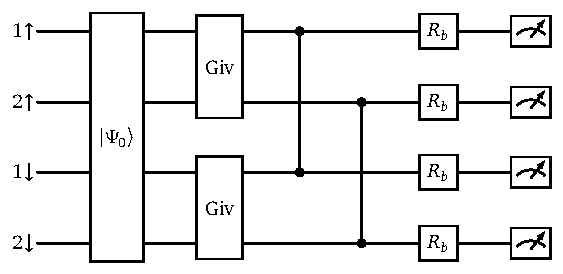
\includegraphics[width=\columnwidth]{figs/fig_circuit_qtk.pdf}
\caption{\textbf{Measurement circuit of the bond-basis moment estimator (schematic; not run on hardware).} One circuit of the estimator of Appendix~\ref{app:estimator}, drawn for a two-site unit cell ($4$ qubits: two spin-up and two spin-down orbitals). The first blocks stand for a state preparation: a reference state $|\Psi_0\rangle$, number-conserving hopping within each spin species ($\mathrm{Giv}$), and the on-site interaction $U\hat n_\uparrow\hat n_\downarrow$ (the controlled pairs, coupling each up orbital to its down partner). A per-qubit basis rotation $R_b$ follows ($H$ or $S^\dagger H$ for the $X$ or $Y$ Pauli components, the identity for $Z$), then a computational-basis measurement. One circuit is needed per qubit-wise-commuting Pauli group. The diagonal density probe gives $m_0$ from the single all-$Z$ setting; the hopping content of $m_1,m_2$ needs the rotated settings ($357$ groups for the full battery at $L=6$; $83$ for the $(m_0,m_1)$ falsifier at $L=12$). The verification of Appendix~\ref{app:estimator} samples the exact ground state in each basis instead of running a preparation circuit. On present hardware the off-diagonal estimate would carry the bias of Sec.~\ref{sec:device}.}
\label{fig:circuit}
\end{figure}

\section{A closed-form bound: the Christoffel miss-distance}
\label{sec:christoffel}

\begin{figure}[t]
\centering
\adjustbox{max width=\textwidth}{% fig_bracketing.tex -- NEW native pgfplots (figure*). The mechanism of Theorem 1:
% finitely many moments BRACKET the cumulative weight F(t); the bracket width IS W_n(t), contracting with n.
% 2026-09-27 layout fix: (i) clip mode=individual, so the t* label sits just above the top frame instead of being
% clipped under it; (ii) the inset is typeset into a box first and placed on the main axis's FOREGROUND layer on an
% opaque white panel inside the empty lower-left region of the main axis (t in [-0.955,-0.70], F in [0.14,0.66]:
% F(t) < 0.03 and both brackets < 0.1 there), so the main grid (drawn on top by axis on top + fillbetween layers)
% no longer shows through the inset and its y label no longer sits on the main 0.4 tick label;
% (iii) inset ymax 1.04 so the n=1 marker (1.000) clears the inset's top frame; (iv) main grid drawn below the data.
% ---- inset: max bracket width vs order (same christoffel_maxW.dat as fig_christoffel (b)) ----
\ifdefined\bracketinsetbox\else\newsavebox\bracketinsetbox\fi
\sbox\bracketinsetbox{%
\begin{tikzpicture}
\begin{axis}[
  width=4.1cm, height=2.95cm,
  paperaxis, grid=none,
  xmin=0.7, xmax=4.3, ymin=0.82, ymax=1.04, xtick={1,2,3,4}, ytick={0.85,0.95},
  xlabel={order $n$}, ylabel={$\max_t W_n$},
  xlabel style={font=\scriptsize}, ylabel style={font=\scriptsize},
  tick label style={font=\scriptsize},
]
  \addplot[pOx, very thick, mark=*, mark size=1.8pt, mark options={fill=pAmber,draw=pOx}]
      table[x=n,y=maxW]{figs/christoffel_maxW.dat};
\end{axis}
\end{tikzpicture}}%
\begin{tikzpicture}
\begin{axis}[
  name=main, paperaxis,
  width=12.4cm, height=6.9cm,
  xmin=-1, xmax=-0.35, ymin=0, ymax=1.03,
  xtick={-1,-0.9,-0.8,-0.7,-0.6,-0.5,-0.4},
  % F(t) and the brackets run to t=1; each plot is clipped to the axis box (clip mode=individual), while the
  % annotation nodes below are not, so the t* label can sit above the top frame
  xlabel={rescaled frequency $t$}, ylabel={cumulative weight $F(t)=\int^{t}\!A$},
  clip=true, clip mode=individual,
  axis on top=false,   % grid below the data: on top, the F=1 grid line split the thick staircase into two thin lines
]
  % n=2 bracket (light amber) = extremal spread over measures sharing m_0..m_4
  \addplot[name path=lo2, draw=none, forget plot] table[x=t,y=Flo]{figs/bracket_env_n2.dat};
  \addplot[name path=hi2, draw=none, forget plot] table[x=t,y=Fhi]{figs/bracket_env_n2.dat};
  \addplot[pAmber, fill opacity=0.26, forget plot] fill between[of=lo2 and hi2];
  % n=4 bracket (deep oxblood) nests inside
  \addplot[name path=lo4, draw=none, forget plot] table[x=t,y=Flo]{figs/bracket_env_n4.dat};
  \addplot[name path=hi4, draw=none, forget plot] table[x=t,y=Fhi]{figs/bracket_env_n4.dat};
  \addplot[pOx, fill opacity=0.34, forget plot] fill between[of=lo4 and hi4];
  % the true cumulative weight lies inside every bracket
  \addplot[pInk, very thick, const plot] table[x=t,y=F]{figs/bracket_F.dat};

  % interior support point t* (dominant atom): guide inside, label just above the top frame (outside the data)
  \draw[guide] (axis cs:-0.5795,0) -- (axis cs:-0.5795,1.0);
  \node[pInk, font=\scriptsize, anchor=south, inner sep=1.5pt] at (axis cs:-0.5795,1.03) {$t^{*}$};

  % labels (short, in the opened whitespace)
  \node[pAmber!75!black, font=\small, anchor=east] at (axis cs:-0.62,0.55) {$n{=}2$};
  \node[pOx, font=\small, anchor=east] at (axis cs:-0.62,0.40) {$n{=}4$};
  \node[pInk, font=\small, anchor=east] at (axis cs:-0.38,0.92) {true $F(t)$};
  \node[pInk, font=\scriptsize, anchor=north west, align=left] at (axis cs:-0.99,0.98)
      {finitely many moments do not\\ pin $F(t)$ --- they \emph{bracket} it;\\ the band width is the\\ Christoffel function $W_n(t)$};

  % the inset, on an opaque white panel above the main grid
  \pgfplotsonlayer{axis foreground}
    \node[fill=white, inner sep=1pt, anchor=south west] at (axis cs:-0.955,0.14) {\usebox\bracketinsetbox};
  \endpgfplotsonlayer
\end{axis}
\end{tikzpicture}
}\\[6pt]
\adjustbox{max width=\textwidth}{% fig_christoffel.tex -- native pgfplots (figure*, full width). Certified Christoffel miss-distance.
% x is the rescaled frequency in [-1,1] (data columns keep the name t; t is the hopping elsewhere in the paper).
% 2026-09-28 (review pass E: V49-02, V49-04, R3-10, notation N1): grid drawn below the data (axis on top=false), so it
% no longer splits the "=" of the (a) labels, the thick (c) segment or the floor label; the (a) labels are footnotesize
% and sit between the x=0.5 grid line and the frame, clear of the y grid lines; the n=1 colour is darkened (the pale
% yellow F4C453 was nearly invisible on white); narrower panels so the row is shrunk less; in (c)
% the points n=5..10 are drawn in a separate grey style: the measure has five weighted atoms
% (christoffel_poles.dat), so H_n is singular for n > 4 and those values (0.778094 in christoffel_floor.dat, computed
% at 60 digits on the full-Fock frequency list whose other atoms carry only round-off weight) lie outside the
% hypothesis H_n > 0 of Theorem 1.
\definecolor{cn1}{HTML}{C9981F}
\definecolor{cn2}{HTML}{D98E32}
\definecolor{cn3}{HTML}{B0360C}
\definecolor{cn4}{HTML}{5A160B}
\begin{tikzpicture}
\begin{groupplot}[
  % 2026-09-27 (m14): the rotated y labels of (b) and (c) touched the right-side ticks of the panel to their
  % left. Right-side y ticks are dropped (they pointed into the gap) and the gap is widened.
  group style={group size=3 by 1, horizontal sep=1.7cm},
  paperaxis, width=5.0cm, height=5.3cm,
  ytick pos=left,
  axis on top=false,   % grid below data and labels
]
% ---- (a) the band W_n(x) contracting ----
\nextgroupplot[
  xlabel={rescaled frequency $x\in[-1,1]$},
  ylabel={bound width $W_n(x)$},
  xmin=-1, xmax=1, ymin=0, ymax=1.06,
  title={\small\textbf{(a)} band contracts with order},
]
  \addplot[cn1, thick] table[x=t,y=W1]{figs/christoffel_Wn.dat};
  \addplot[cn2, thick] table[x=t,y=W2]{figs/christoffel_Wn.dat};
  \addplot[cn3, thick] table[x=t,y=W3]{figs/christoffel_Wn.dat};
  \addplot[cn4, very thick] table[x=t,y=W4]{figs/christoffel_Wn.dat};
  % curve labels: between the x=0.5 grid line and the frame, clear of the y = 0.5 and 1 grid lines
  \node[cn1, font=\footnotesize, anchor=west, inner sep=1pt] at (axis cs:0.56,0.93) {$n{=}1$};
  \node[cn2, font=\footnotesize, anchor=west, inner sep=1pt] at (axis cs:0.56,0.81) {$n{=}2$};
  \node[cn3, font=\footnotesize, anchor=west, inner sep=1pt] at (axis cs:0.56,0.69) {$n{=}3$};
  \node[cn4, font=\footnotesize, anchor=west, inner sep=1pt] at (axis cs:0.56,0.57) {$n{=}4$};
% ---- (b) max_x W_n shrinking ----
\nextgroupplot[
  xlabel={polynomial order $n$},
  ylabel={$\max_x W_n(x)$},
  xmin=0.7, xmax=4.3, ymin=0.82, ymax=1.02,
  xtick={1,2,3,4},
  title={\small\textbf{(b)} tighter with more moments},
]
  \addplot[pOx, very thick, mark=*, mark size=2.6pt, mark options={fill=pAmber,draw=pOx}]
      table[x=n,y=maxW]{figs/christoffel_maxW.dat};
% ---- (c) W_n at the dominant pole saturates at the residue ----
\nextgroupplot[
  xlabel={polynomial order $n$},
  ylabel={$W_n$ at dominant pole},
  xmin=0.5, xmax=10.5, ymin=0.66, ymax=1.04, ytick={0.7,0.8,0.9,1},
  xtick={1,3,5,7,9},
  title={\small\textbf{(c)} saturates, does not vanish},
]
  \addplot[guide, forget plot] coordinates {(0.5,0.7781) (10.5,0.7781)};
  % n = 1..4: H_n positive definite (five weighted atoms)
  \addplot[pIndigo, very thick, mark=*, mark size=2.4pt, mark options={fill=white,draw=pIndigo},
           restrict x to domain=0.5:4.5]
      table[x=n,y=Wn_at_pole]{figs/christoffel_floor.dat};
  % n = 5..10: H_n singular for this measure; drawn separately (small grey markers only)
  \addplot[only marks, mark=*, mark size=1.5pt, mark options={fill=pMuted, draw=pMuted},
           restrict x to domain=4.5:10.5]
      table[x=n,y=Wn_at_pole]{figs/christoffel_floor.dat};
  \node[pInk, font=\scriptsize, anchor=south west, align=left] at (axis cs:4.9,0.80)
      {residue floor\\ $0.778$};
  \node[pMuted, font=\scriptsize, anchor=north west, align=left] at (axis cs:4.9,0.762)
      {grey, $n>4$:\\ $H_n$ singular};
\end{groupplot}
\end{tikzpicture}
}
\caption{\textbf{The Christoffel miss-distance bound at exact moments.} \emph{Top---the bracketing mechanism.} Finitely many moments do not pin the spectrum; they \emph{bracket} its cumulative weight $F(t)$ (ink staircase) between the extremal Gauss--Radau measures sharing $m_0,\dots,m_{2n}$. The band width is the Christoffel function $W_n(t)$; the $n{=}4$ band (deep) nests inside the $n{=}2$ band (light), and $t^{*}$ marks the dominant atom. \emph{Bottom (a--c)---the bound quantified.} \textbf{(a)} $W_n(t)=1/\sum_{j=0}^{n}p_j(t)^2$ contracts as $n$ grows. \textbf{(b)} Its maximum over $t$ decreases with $n$: $1.000$, $0.969$, $0.886$, $0.882$ for $n=1,\dots,4$ (exact maxima, by root-finding). At the deployed order $n=1$ the maximum is $W_1=m_0$, attained at the mean frequency, so there the bracket is vacuous. \textbf{(c)} At the dominant atom ($\omega=11.09\,t$, residue $0.778$) $W_n$ reaches the residue at $n=4$ and stays there: the measure has five weighted atoms, and the bracket at an atom never falls below the jump of $F$ it carries. Pointwise $W_n\to0$ is a thermodynamic-limit statement for a continuous density, not a property of a finite atomic spectrum. All curves assume exact moments; a reconstruction that passes with finite tolerances is bracketed less tightly (see text). Doped Hubbard $L=6$, $U/t=8$ current Lehmann measure, normalized to $m_0=1$ (the ground state is a spin triplet; the measure is the same for each of its $S_z$ components), rescaled to $t\in[-1,1]$ from the full-Fock frequency range $[0.148,52.21]\,t$, zero-weight states included, so the weighted atoms occupy $t\in[-0.91,-0.47]$~\cite{GM2010,ShohatTamarkin1943,Akhiezer1965,Totik2000,MNT1991,Szego1975}.}
\label{fig:bracketing}
\label{fig:christoffel}
\end{figure}

Having shown empirically what the screen catches, we now state what a \emph{passing} screen implies. The bound below is classical, from the theory of moments and orthogonal polynomials. Our contribution is its evaluation as a diagnostic for a reconstructed spectrum, not the mathematics; the Christoffel--Darboux kernel is by now an established data-analysis tool in its own right~\cite{GM2010,Szego1975,PauwelsLasserre2019,LasserrePauwelsPutinar2022}. Consider the cumulative spectral weight $F(t) = \int_{-\infty}^{t} A(\omega)\,d\omega$ of a diagonal $T=0$ Lehmann measure, and suppose the first $2n{+}1$ moments $m_0,\dots,m_{2n}$ are known exactly. They fix the orthonormal polynomials $p_0,\dots,p_n$ via the Hankel system~\cite{ShohatTamarkin1943}. Let $W_n(t) = 1/\sum_{j=0}^{n} p_j(t)^2$ be the Christoffel function, also written $\lambda_n(t)\equiv W_n(t)=1/K_n(t,t)$ with $K_n(x,y)=\sum_{j=0}^{n}p_j(x)p_j(y)$ the Christoffel--Darboux kernel; its construction from the moments is given in Appendix~\ref{app:evaluate}~\cite{Szego1975,GM2010}.

\begin{theorem}[Cumulative-weight miss-distance bound (classical; re-derived)]
Let $d\mu=A(\omega)\,d\omega$ be a positive measure of compact support (a diagonal $T=0$ Lehmann spectrum) whose Hankel matrix $H_n=[m_{i+j}]_{i,j=0}^{n}$ is positive definite, and suppose the moments $m_0,\dots,m_{2n}$ are known exactly. For $t\in\mathbb{R}$ define the cumulative-weight miss-distance as the extremal spread $\sup|F_{\nu_1}(t)-F_{\nu_2}(t)|$ over all positive measures $\nu_1,\nu_2$ on $\mathbb{R}$ sharing those moments. Then for every $t\in\mathbb{R}$ this spread equals the Christoffel function $W_n(t)$, which is also the supremum of the mass a moment-matching measure can place at $t$ (the Gauss--Radau weight $\lambda_n(t)$, attained except at the $n$ zeros of the orthonormal polynomial $p_n$). In particular, any reconstruction whose moments $m_0,\dots,m_{2n}$ equal the true ones obeys $|F_{\mathrm{rec}}(t)-F_{\mathrm{true}}(t)|\le W_n(t)$ at every $t\in\mathbb{R}$ (Appendix~\ref{app:proof})~\cite{KarlinStudden1966,DetteStudden1997}.
\end{theorem}

\noindent\emph{Remarks.} The equality needs no convex-hull hypothesis. Once $H_n\succ0$, a Gauss--Radau rule with positive weights and a node prescribed at $t$ exists for every real $t$ other than the $n$ zeros of $p_n$, and its atom at $t$ is $W_n(t)$; at those zeros the same value is approached as a limit (Appendix~\ref{app:proof}). We checked this on the measure of Fig.~\ref{fig:christoffel}: all $24$ rules tested ($n=1,\dots,4$; $20$ of them with $t$ outside the hull of the weighted atoms) have positive weights, reproduce $m_0,\dots,m_{2n}$ to $1.4\times10^{-17}$, and carry an atom equal to $W_n(t)$ to $2\times10^{-16}$. The bound is monotone, $W_{n+1}(t)\le W_n(t)$, since $K_{n+1}\ge K_n$. For a spectrum of $N$ distinct poles $H_n\succ0$ only for $n\le N-1$, and at a pole $\omega_i$ one has $W_n(\omega_i)\ge w_i>0$ (the residue), with equality at $n=N-1$; $W_n$ does not vanish on the support. Pointwise vanishing $W_n(t)\to0$ is a thermodynamic-limit statement. If the discrete spectrum densifies to a measure that is Stahl--Totik regular with compact support $S$ and absolutely continuous with a density $A$ obeying the local Szeg\H{o} condition $\int_I\log A>-\infty$ on an interval $I\subset S$, then $n\,W_n(x)\to A(x)/\omega_S(x)$ for almost every $x\in I$, with $\omega_S$ the equilibrium density of $S$~\cite{Totik2000}; on a single interval this reduces to M\'at\'e--Nevai--Totik~\cite{MNT1991}.

The equality is the classical content of the Chebyshev--Markov--Stieltjes inequalities and of Gauss--Christoffel moment theory, re-derived in Appendix~\ref{app:proof}~\cite{GM2010,ShohatTamarkin1943,Akhiezer1965}. We say ``bound'', not ``certify'': the screen never certifies that $A(\omega)$ is correct. The bounded object is cumulative weight, not the pointwise value of $A(\omega)$ or the position of a peak~\cite{GM2010}, and the contraction \emph{rate} holds only under the regularity hypothesis above~\cite{Totik2000,MNT1991}. The top panel of Fig.~\ref{fig:christoffel} shows the mechanism: the true $F(t)$ lies between the Gauss--Radau extremal envelopes of all measures sharing the moments, and the width of that bracket is $W_n(t)$.

The theorem assumes exact moments, and the deployed screen does not supply them. If a reconstruction's moments $m_0,\dots,m_{2n}$ equal the true ones, its $F(t)$ is pinned within $W_n(t)$. The screen instead passes a reconstruction whose residuals lie within tolerances, $|\Delta_k|\le\tau_k$, and only through order $2n=2$. Two consequences follow for the measure of Fig.~\ref{fig:christoffel}. First, at the deployed order $n=1$ the exact-moment bracket is the one-sided Chebyshev (Cantelli) bound, $W_1(\omega)=m_0\,\sigma^2/[\sigma^2+(\omega-\bar\omega)^2]$ with mean $\bar\omega=11.10\,t$ and variance $\sigma^2=2.10\,t^2$ (this closed form and the orthogonal-polynomial evaluation agree to $1.6\times10^{-15}$). Its maximum is $m_0$, at the mean, which here lies $0.01\,t$ from the dominant atom ($11.09\,t$), so the bracket is vacuous at the peak; just above the top pole, at $\omega=14\,t$, it is still $0.20$. Second, tolerances loosen it further. The largest atom that a positive measure with $|m_k-m_k^{\mathrm{true}}|\le\tau_k$ ($k\le2$, the deployed threshold rule evaluated on this state) can place at $\omega$ is $3.2$--$7.7$ times $W_1$ at $\omega=14$--$20\,t$ ($0.63$ against $W_1=0.20$ at $14\,t$) and $10$--$11$ times $W_1$ far outside the band ($\omega\approx34$--$50\,t$); at the mean it exceeds $m_0$ ($1.045\,m_0$). At exact-moment orders $n\le4$ ($m_0,\dots,m_8$) the global maximum falls only to $\max_tW_4=0.882$, and at $n=N-1=4$ the value of $W_4$ at the dominant atom already equals its residue $0.778$ and stays there (panel~c). No positive-order moment beyond $m_2$ is estimated in this work. At the deployed order, passing the screen therefore places no constraint on the cumulative weight at the peak. This is the moment-level counterpart of the companion's finding that captured weight alone cannot certify a sample-based spectral function~\cite{SQDspec2608}.

Refutation and bracketing are separate statements. A reconstruction is rejected when some $|\Delta_k|$ exceeds $\tau_k$; that test does not involve $W_n$, and its reach is set by the thresholds (Sec.~\ref{sec:detect}). A Hankel/Stieltjes violation of the \emph{estimated} moments rejects the estimate, not a non-negative reconstruction, whose own moments satisfy positivity by construction. $W_n$ governs only the complementary statement, how tightly a \emph{passing} reconstruction's cumulative weight is bracketed. The looseness above therefore limits what passing implies; it does not limit the power to reject.

The bracket is not uniformly loose. At a frequency the measure leaves empty, $W_n(t)$ bounds the weight that any moment-matching reconstruction can place there. The rescaled frame of Fig.~\ref{fig:christoffel} maps the full-Fock range $[0.148,52.21]\,t$ onto $[-1,1]$; the weighted atoms occupy $t\in[-0.91,-0.47]$, and $73.5\%$ of the axis lies above the top pole ($13.9\,t$). At the rescaled points $t=0.3$, $0.6$ and $0.9$ in that empty region ($\omega=34.0$, $41.8$ and $49.6\,t$) the $60$-digit evaluation of App.~\ref{app:evaluate} gives $W_1=4.0\times10^{-3}$, $2.2\times10^{-3}$ and $1.4\times10^{-3}$, and at $t=0.6$ the higher orders give $W_2=1.4\times10^{-5}$, $W_3=2.7\times10^{-8}$ and $W_4=3.6\times10^{-10}$. These small values reflect the distance from the band, not resolution: at $n=1$ they are the Cantelli tail. Nearer the band the bracket is wider ($W_1=0.20$ at $\omega=14\,t$), and the deployed tolerances raise the far-out-of-band $n=1$ values about tenfold. This is a computed property of this measure, not a theorem, and we do not extrapolate it to the two-sided single-particle Mott gap, a distinct measure not tested here.

\begin{proposition}[Two-sided Markov--Krein window-mass bound]
\label{prop:markovkrein}
Let $d\mu=A(\omega)\,d\omega$ be a positive measure (a diagonal $T=0$ Lehmann spectrum) with $H_n=[m_{i+j}]_{i,j=0}^{n}\succ0$, and suppose $m_0,\dots,m_{2n}$ are known exactly. For any frequency window $[c,d]$ with $c\le d$ real, the mass $\mu([c,d])=\int_c^d A(\omega)\,d\omega$ of \emph{every} positive measure sharing those moments obeys
\begin{equation}
\begin{aligned}
\max\{0,\,F_-(d)-F_+(c)\}\ &\le\ \mu([c,d])\\
&\le\ \min\{m_0,\,F_+(d)-F_-(c)\},
\end{aligned}
\label{eq:mk-window}
\end{equation}
where $F_\pm(t)$ are the lower/upper principal (Gauss--Radau) cumulative representations of Lemma~3 (App.~\ref{app:proof}): $F_-(t)$ is the mass that the $(n{+}1)$-point Gauss--Radau rule with a node fixed at $t$ places strictly left of $t$, and $F_+(t)=F_-(t)+\lambda_n(t)$ with $\lambda_n(t)=W_n(t)$ its atom at $t$ (at the $n$ zeros of $p_n$, where that rule degenerates, both are taken as limits). The bracket is two-sided. Its width is at most $W_n(c)+W_n(d)$ (with equality before intersecting with the trivial bounds $[0,m_0]$), so it inherits the monotone contraction $W_{n+1}\le W_n$ and is tight wherever \emph{both} endpoints fall in weight-poor frequency. The sharp Krein--Nudelman extremum, attained by a principal representation with prescribed nodes at $c$ and $d$ (equivalently, the optimum of the scalar truncated-moment problem over positive measures), is no wider. Equation~\eqref{eq:mk-window} follows directly from the Chebyshev--Markov--Stieltjes inequalities and extends the one-sided point bound $|F_{\mathrm{rec}}-F_{\mathrm{true}}|\le W_n$ to a two-sided bound on integrated weight~\cite{KreinNudelman1977,KarlinStudden1966,DetteStudden1997,GM2010}.
\end{proposition}

We evaluated the two-sided bracket~\eqref{eq:mk-window} on the same $L=6$, $U/t=8$ current measure (App.~\ref{app:evaluate}; committed script \texttt{markov\_krein\_window.py}), again at exact moments. At $n=4$ ($m_0,\dots,m_8$), a window with one edge at the $400$-point-grid maximizer of $W_4$, just above the dominant atom, gives $\mu\in[0.070,0.945]$, width $0.875$; the exact maximum of $W_4$, at a nearby frequency, is $0.882$. A window that contains the peak with both edges in weight-free frequency (rescaled $[-0.75,-0.35]$) gives $\mu\in[0.9732,0.9758]$ around the exact $0.9744$, and the empty window rescaled $[0.3,0.9]$ ($\omega\approx34$--$50\,t$) gives $\mu\in[0,3.2\times10^{-9}]$. At the deployed order $n=1$ ($m_0,m_1,m_2$) the peak-containing window gives $\mu\in[0.848,1]$ and the empty window $\mu\in[0,0.004]$, while a window with an edge on the peak is uninformative (its bracket runs from $0$ to within $2\times10^{-4}$ of $m_0$). These are exact-moment brackets. Under the deployed tolerances the upper end for the empty window is at least $0.040$, the largest atom that a measure with $m_0,m_1,m_2$ within tolerance can place at its lower edge ($\omega\approx34\,t$). The two-sided bound is thus tight when both window edges lie where $W_n$ is small, and as loose as $W_n$ when an edge sits on the peak. It is the real-axis, ground-state-moment counterpart of the Euclidean-time two-sided spectral bounds recently obtained from moment-problem semidefinite programs~\cite{CausalBootstrap2026,CertifiedSpectral2026,AbbottJayOare2025}; it differs in that its moments are ground-state operator expectations rather than lattice correlators. As with the one-sided bound, we do not extrapolate it to the two-sided single-particle Mott gap.

\section{Detectability and its sample-complexity limit}
\label{sec:detect}
The Christoffel bound of Sec.~\ref{sec:christoffel} concerns what a passing screen implies: how tightly a \emph{passing} spectrum's integrated weight is bracketed. Rejection has a matching characterization. It states which reconstruction errors the moment battery can detect in exact arithmetic, and what it can guarantee at finite thresholds, where the Vandermonde structure of the moment map sets the shot cost. The limiting error class is the \emph{within-sector redistribution}: a corruption that keeps the retained determinant support (so the leakage estimator of Sec.~\ref{sec:teeth} is blind by construction) and only reweights the reconstructed poles. The statement below is not a new theorem. Part~(a) restates the classical Prony/Vandermonde uniqueness of an atomic measure from its moments~\cite{ShohatTamarkin1943,PottsTasche2013}; part~(b) turns it, together with an elementary shifted-power bound, into a detectability-versus-shot-budget statement for the battery. We keep the \texttt{theorem} environment for cross-referencing.

\begin{theorem}[Detectability and completeness of the moment battery]
\label{thm:detect}
Let $A(\omega)=\sum_{n=1}^{N}w_n\,\delta(\omega-\omega_n)$ be a diagonal $T=0$ Lehmann measure on $N$ \emph{distinct} poles $\{\omega_n\}$ with $w_n=|\langle n|J|0\rangle|^2\ge0$, and let a within-sector redistribution $\mathbf{w}\to\mathbf{w}+\bm{\delta}$ ($\bm{\delta}\neq0$, keeping $w_n+\delta_n\ge0$) act on the \emph{same} poles. Write $\mathbf{m}=V\mathbf{w}$ with $V_{kn}=\omega_n^{\,k}$, the induced shift $\Delta_k=|(V\bm{\delta})_k|=\big|\sum_n\delta_n\,\omega_n^{\,k}\big|$, and $\rho=\|\bm{\delta}\|_1$. Then $\|\bm{\delta}\|_2\le\rho\le\sqrt{N}\,\|\bm{\delta}\|_2$, and $\rho/2$ is the weight moved when $m_0$ is preserved.
\begin{enumerate}
\item[(a)] \emph{(Completeness in exact arithmetic.)} If the redistribution preserves $m_0,\dots,m_K$ with $K<N-1$, then $\Delta_j>0$ for at least one $j$ with $K<j\le N-1$; quantitatively
\begin{equation}
\max_{K<j\le N-1}\Delta_j\ \ge\ \frac{\sigma_{\min}(V_{0:N-1})}{\sqrt{N-1-K}}\;\|\bm{\delta}\|_2,
\label{eq:detect-sigmamin}
\end{equation}
with $V_{0:N-1}$ the $N\times N$ node-Vandermonde on rows $0,\dots,N-1$ and both sides in one fixed frequency unit. Hence the order-$(N{-}1)$ battery is \emph{complete} for fixed-pole redistributions: no nonzero within-sector redistribution preserves all of $m_0,\dots,m_{N-1}$. If the poles may also move (two measures of at most $N$ atoms each), completeness holds at order $2N-1$ by Prony counting~\cite{ShohatTamarkin1943,PottsTasche2013}. The only alteration invisible to every moment is weight traded among degenerate eigenstates at one frequency, which leaves $A(\omega)$ unchanged and is not an error.
\item[(b)] \emph{(Finite thresholds.)} Let each moment carry the noise floor $\delta_k=\sqrt{\operatorname{Var}(O_k)/N_s+b_k^2}$ at $N_s$ shots, with bias budget $b_k$, and the two-sided threshold $\tau_k=z_{1-\alpha/2}\,\delta_k$. We call a given $\bm{\delta}$ \emph{exposed} at order $j$ when its noise-free shift exceeds the threshold, $\Delta_j>\tau_j$; whether a finite-shot test then rejects it is a question of power (Corollary below). Some $m_0,\dots,m_K$-preserving redistribution is exposable at order $K{+}1$ iff $\Delta_{K+1}^{\max}>\tau_{K+1}$, with $\Delta_{K+1}^{\max}$ the linear program~\eqref{eq:wclp}. If rows $0,\dots,K{+}1$ of $V$ have a nontrivial null space ($N-K-2\ge1$), the smallest $\Delta_{K+1}$ over such redistributions is zero for every size $\rho$ up to a limit set by positivity: the guaranteed power at order $K{+}1$ is zero, however well separated the poles. Two conditions bracket detection.
\par\emph{(i) Sufficient.} If $\bm{\delta}$ preserves $m_0,\dots,m_K$, it is exposed at some order $j\le N-1$ whenever the right-hand side of~\eqref{eq:detect-sigmamin} exceeds $\max_{K<j\le N-1}\tau_j$.
\par\emph{(ii) Necessary (cluster bound).} If $\bm{\delta}$ preserves $m_0,\dots,m_{s-2}$ and is supported on poles within an interval of diameter $D$ and midpoint $\omega_c$, then $(V\bm{\delta})_{s-1}=\sum_n\delta_n(\omega_n-\omega_c)^{s-1}$, so $\Delta_{s-1}\le\rho\,(D/2)^{s-1}$; every higher shift obeys $\Delta_j\le\rho\sum_{i=s-1}^{j}\binom{j}{i}|\omega_c|^{j-i}(D/2)^{i}$, which is also $O(\rho D^{s-1})$. Exposure at order $s-1$ therefore requires
\begin{equation}
\begin{aligned}
\rho&\,>\,\frac{\tau_{s-1}}{(D/2)^{s-1}},\qquad\text{equivalently}\\[3pt]
N_s&\,>\,\frac{z_{1-\alpha/2}^{2}\,\operatorname{Var}(O_{s-1})}{\rho^2(D/2)^{2(s-1)}-z_{1-\alpha/2}^2\,b_{s-1}^2},
\end{aligned}
\label{eq:detect-Ns}
\end{equation}
and no $N_s$ suffices when $\rho\,(D/2)^{s-1}\le z_{1-\alpha/2}\,b_{s-1}$. The shot cost to detect a redistribution of fixed size at its first exposable order grows at least as $D^{-2(s-1)}$ as the cluster contracts.
\end{enumerate}
\end{theorem}

\noindent\emph{Proof sketch.} Part~(a): distinct poles make $V_{0:N-1}$ an invertible Vandermonde, so $V_{0:N-1}\bm{\delta}=0$ forces $\bm{\delta}=0$. Preserving $m_0,\dots,m_K$ zeroes the first $K{+}1$ components of $V_{0:N-1}\bm{\delta}$, whence $\|(\Delta_{K+1},\dots,\Delta_{N-1})\|_2=\|V_{0:N-1}\bm{\delta}\|_2\ge\sigma_{\min}(V_{0:N-1})\|\bm{\delta}\|_2$, and~\eqref{eq:detect-sigmamin} follows from $\ell_2\!\to\!\ell_\infty$. The moving-pole count is the classical uniqueness of an $N$-atom measure given $m_0,\dots,m_{2N-1}$. Part~(b): a vector in the null space of rows $0,\dots,K{+}1$, scaled so that $w_n+\delta_n\ge0$, preserves $m_0,\dots,m_{K+1}$, which gives the zero guaranteed power; (i) compares~\eqref{eq:detect-sigmamin} with $\max_j\tau_j$. For (ii), expand $\omega^{j}=\sum_i\binom{j}{i}\omega_c^{\,j-i}(\omega-\omega_c)^i$. The terms with $i\le s-2$ are combinations of preserved moments and vanish, and $|\omega_n-\omega_c|\le D/2$ on the support bounds the rest; inserting $\tau_{s-1}=z_{1-\alpha/2}\,\delta_{s-1}$ gives~\eqref{eq:detect-Ns}. The linear program~\eqref{eq:wclp} and the numerical instance are in Appendix~\ref{app:withinsector}.

\noindent\emph{Remarks.} The clustered-node bounds $\sigma_{\min}\sim\Delta\omega^{\,s-1}$ of super-resolution theory, with $\Delta\omega$ the node spacing~\cite{Moitra2015,BatenkovClustered2020,KunisNagel2021,Donoho1992}, are proved for Fourier-type nodes on the unit circle or torus, not for the real nodes of power moments, and part~(b)(ii) does not rely on them. For real nodes the same scaling, $\sigma_{\min}\propto D^{s-1}$ for the $s\times s$ Vandermonde of a cluster at fixed relative geometry, follows from Gautschi's inverse-Vandermonde bound~\cite{Gautschi1962,Gautschi1963} together with the shifted-power identity (Appendix~\ref{app:withinsector}). Numerically, for $s$ equally spaced nodes at the median pole of the $L=6$ instance below, $\sigma_{\min}$ falls with the spacing with fitted exponents $0.995$, $1.98$ and $2.96$ for $s=2,3,4$. For an isolated cluster, then, the sufficient condition~(i) weakens with the same power of the spacing as the necessary bound~(ii). If a cluster contracts uniformly, so that its minimal pole separation falls from $\Delta\omega_{\min}$ to $\Delta\omega$, $D$ shrinks by the same factor and the lower bound~\eqref{eq:detect-Ns} on the shot cost grows by at least $(\Delta\omega_{\min}/\Delta\omega)^{2(s-1)}$. A finite separation below which no budget suffices exists only with a bias floor, $b_{s-1}>0$. Finally, the fixed-pole class excludes under-converged Krylov reconstructions. A reconstruction on a subspace containing the order-$K$ Krylov space reproduces $m_0,\dots,m_{2K+1}$ exactly~\cite{SQDspec2608}; a Lanczos representation with $K{+}1$ nodes is such a reconstruction. With two or more nodes it therefore matches the whole deployed battery by construction, whatever its line-shape error; the one-node case matches only $m_0,m_1$, misses $m_2$ by $2$--$4\%$, and passes within a threshold that budgets a $2\%$ bias (largest residual $0.99\,\tau_2$). This accounts for the Krylov misses of Sec.~\ref{sec:blind}; Theorem~\ref{thm:detect} does not cover them because the poles move.

\medskip
\noindent\emph{Corollary (detection power vs.\ cluster size and shot count).}\enspace Under the Gaussian estimator validated in Fig.~\ref{fig:momentmc} (skewness $-0.04$, excess kurtosis $-0.05$), the test reaches power $1-\beta$ at level $\alpha$ when $\Delta_j\gtrsim z_{\alpha,\beta}\,\delta_j$, with $z_{\alpha,\beta}=z_{1-\alpha/2}+z_{1-\beta}$ and the bias budget counted in $\delta_j$ as in the deployed rule. By part~(b)(ii) this requires $N_s\gtrsim z_{\alpha,\beta}^2\operatorname{Var}(O_{s-1})/[\rho^2(D/2)^{2(s-1)}-z_{\alpha,\beta}^2 b_{s-1}^2]$ at the first exposable order, and no budget suffices below the bias-limited cluster diameter $D_\star=2\,(z_{\alpha,\beta}\,b_{s-1}/\rho)^{1/(s-1)}$. Without bias the cost is finite for every $D>0$ and diverges only as $D\to0$.

For the deployed $L=6$, $U/t=4$ battery the $N=5$ poles are well separated (minimal separation $\Delta\omega_{\min}=0.87\,t$; on nodes rescaled to $[-1,1]$, $\sigma_{\min}(V_{0:4})=0.056$ and $\kappa=50$), yet the guaranteed power of the deployed battery against fixed-pole redistribution is zero. The reason is the null-space dimension, not conditioning: rows $0,1,2$ of $V$ leave a two-dimensional null space on five poles. Over $m_0,m_1$-preserving redistributions the linear program~\eqref{eq:wclp} gives the signed shift of $m_2$ in $[-0.92,7.09]$ (Table~\ref{tab:withinsector}). The largest shift is $3.8\,\tau_2$ ($\tau_2=1.848$), but the range contains zero. Three explicit redistributions pass the deployed battery. CE1 lies in that null space: it preserves $m_0,m_1,m_2$ exactly while moving $72\%$ of the weight ($\rho=1.43\,m_0$), emptying two of the five poles and cutting the dominant residue from $0.393$ to $0.037$. CE2 preserves $m_0,m_1$ and sets $\Delta_2=\tau_2$ while moving $86\%$ of the weight (dominant residue $0.393\to0.073$). CE3 holds every residual at or within its threshold and empties three poles, the dominant one included. The random redistribution committed with the original analysis also passes: it moves $25\%$ of the weight with $\Delta_2=0.044\,\tau_2$. Orders $3$ and $4$ would catch some of these, but not all. With the same rule ($\tau_3=15.0$, $\tau_4=122$; the local-estimator variance behind them is a lower bound), CE2 and CE3 give $\Delta_3\approx3.3\,\tau_3$ and $\Delta_4\approx7.1$--$7.2\,\tau_4$, whereas CE1 gives $0.23\,\tau_3$ and $0.70\,\tau_4$. Over all redistributions that keep $m_0,m_1,m_2$ exactly, $\Delta_3\le0.35\,\tau_3$, and $\Delta_4$ reaches $1.19\,\tau_4$ at the one that maximizes $\Delta_3$, a marginal case. Neither $m_3$ nor $m_4$ is estimated in this work. The sufficient condition~(i) is far from met here: for CE1 and CE2 the right-hand side of~\eqref{eq:detect-sigmamin} is below $4\times10^{-3}$, against $\max_j\tau_j=\tau_4=122$ in the same units. The residual blind spot of the deployed screen therefore has two sources. The first is the battery order: with $m_0,\dots,m_K$, every fixed-pole redistribution in the $(N-K-1)$-dimensional null space passes, regardless of pole separation. The second is pole clustering, which by~\eqref{eq:detect-Ns} raises the shot cost of detection at least as $D^{-2(s-1)}$. Injectivity guarantees that some $m_j$ separates any fixed-pole redistribution; the thresholds decide whether that separation is observable at a given budget.

\section{Discussion and limitations}\label{sec:limits}
This paper contributes a method with stated operating limits: a reconstruction-independent moment screen for sample-based quantum spectral functions; estimators that evaluate the moments without reading them off $A(\omega)$, either as full-operator expectation values on the sampled subspace state (classical post-processing) or from separate bond-basis measurements on a prepared ground state (simulated only, Appendix~\ref{app:estimator}); a hash-sealed, blinded calibration of the screen's detection and false-positive rates where the truth is known; and classical bounds that state what a passing screen does and does not imply. The screen is a necessary condition. Failing it rejects the reconstruction at the pre-registered level (per-moment $\alpha=0.05$; blinded false-positive rate $0.9\%$, $1/112$). Passing it excludes only the tested failure modes. Independence from $A(\omega)$ is what allows the two branches to disagree; it does not turn agreement into a statement about the line shape.

\emph{Relation to the companion study.} The companion~\cite{SQDspec2608} develops an a posteriori error theory for the same class of sample-based spectral functions, and several of its results bear directly on this screen. Its captured weight $w$ gives our coverage residual as $\Delta_0=m_0(1-w)$. Its moment-exactness theorem---a subspace that contains the order-$K$ Krylov space of the probe reproduces the exact spectral moments through order $2K{+}1$---explains why the under-converged Krylov reconstructions of Sec.~\ref{sec:blind} with two or more Lanczos nodes pass our battery by construction (none of $56$ caught); the one-node reconstructions reproduce only $m_0$ and $m_1$ exactly and pass within the bias budget (none of $15$ caught). Its leakage identity $\mu_2-\mu_2^{\mathcal S}=\lVert Q_{\mathcal S}HP_{\mathcal S}\varphi\rVert^2$ is our operator leak, Eq.~\eqref{eq:app-leak}, at $k=2$ when the probe state lies in $\operatorname{span}\mathcal S$. And its result that captured weight alone cannot certify the reconstruction has a device-data instance here: the $50$k run of Sec.~\ref{sec:device} has $\Delta_0=0.0044$ and a relative $L_1$ error of $0.35$ in $A(\omega)$ at broadening $\eta=0.15\,t$. What this paper adds is (i) the use of low-order moments, evaluated independently of the reconstruction, as a test that applies to any reconstructed $A(\omega)$ and not only to Rayleigh--Ritz on a determinant subspace; its first and second moments detect weight moved in frequency at fixed total weight, which the captured weight cannot see; (ii) a sealed, blinded calibration of that test, with its failures reported; (iii) classical brackets on what passing implies, and the result that the deployed order has zero guaranteed power against fixed-pole weight redistributions; and (iv) an evaluation of the coverage channel on a device-sampled support against reference distributions, which shows that this channel cannot distinguish a good device from one that merely spreads its samples.

The method must be positioned by mechanism against two neighboring approaches, because all three aim to verify quantum results without a classical reference. Self-verifying variational simulation certifies a prepared \emph{state} through an energy-variance bound measured on the device~\cite{Kokail2019}. Observable-estimation validation certifies error-mitigated \emph{expectation values} by validating the hardware noise model and the mitigation procedure~\cite{OEACV2026}. Our screen certifies neither. It tests a reconstructed spectral \emph{function} against operator moments evaluated independently of it, and it targets weight misassignment in subspace reconstructions. For sample-based spectral functions this failure mode is documented by the companion~\cite{SQDspec2608}; for subspace methods in general it is our extrapolation from the limitations documented for their ground-state energies~\cite{Reinholdt2025,Epperly2022,Kirby2024,GaberleJattana2026,VaqueroSabater2026}. The other two approaches do not address it. A separate, non-physical layer verifies the numerical linear algebra of the classical diagonalizer, cross-checking eigenpairs across independent LAPACK paths and sealing the result with tamper-evident certificates~\cite{CertifyED2026}. It catches software and floating-point errors in the solver and, because it acts only on the classical computation, is blind to sampling incompleteness and weight misassignment. The physical approaches are complementary: a hardware spectrum could be produced under observable-estimation validation~\cite{OEACV2026}, prepared with self-verification of its input state~\cite{Kokail2019}, and then screened for weight misassignment by our moments. We claim only the third role.

One may ask why a finished reconstruction should be screened at all, rather than building the moment information \emph{into} the reconstruction so that no inconsistent spectrum is produced. This is the strategy of a mature family of analytic-continuation methods. Nevanlinna continuation imposes the interpolation and Pick/positivity structure of a causal response function, returning spectra that are consistent by construction~\cite{Fei2021}; maximum-entropy and stochastic analytic continuation regularize the ill-posed inversion with moment and sum-rule constraints supplied as prior information~\cite{Jarrell1996,Sandvik1998}; and Prony, minimal-pole and stochastic-pole-expansion methods fit the data to a compact pole model whose low-order moments can be pinned to their operator values~\cite{ZhangGull2024,HuangLiang2023}. Where such a moment-constrained reconstruction is available it is preferable, and our screen does not compete with it. A moment-constrained reconstruction is, however, consistent only with the moments \emph{it} was given, only within the method that enforced them, and only for the imaginary-axis or time-domain data it was built from. A downstream consumer of a quantum-generated spectrum typically receives a finished $A(\omega)$ from a pipeline it does not control and cannot re-run. Our screen is built for that setting: a reconstruction-independent necessary condition attachable to any spectrum, however it was produced, that draws its discriminating power from moments evaluated independently of the reconstruction. Building the moments into the reconstruction and screening the result against independently evaluated moments are two layers of one defense, not alternatives.

A related complementarity has appeared on the device side. Irmejs and Santos propose constructing dynamical correlation functions directly on hardware, without real-time evolution, from a continued-fraction representation whose level-$k$ approximant is a weight-$O(k)$ operator---a spectral moment---measured on a prepared eigenstate; they prove exponential accuracy in a region of the complex-frequency plane bounded away from the real axis and demonstrate the method in classical simulations of small lattices~\cite{IrmejsSantos2025}. A related circuit-differentiation framework builds the retarded Green's function from derivatives of real-time-evolution circuits under realistic noise~\cite{Piccinelli2026}. These are \emph{constructive} programs: they use the same weight-$O(k)$ operator moments to build a response function with a priori convergence guarantees off the real axis. Our screen is their diagnostic counterpart. It assumes no control over how the spectrum was produced and constructs nothing; it takes a finished, real-axis $A(\omega)$ from a sample-based-diagonalization or Krylov pipeline and asks only whether that function is consistent with independently evaluated moments, on the real axis, where the constructive guarantees are weakest.

The Christoffel bound states what passing implies, and its scope is narrow. At exact moments $m_0,\dots,m_{2n}$ the cumulative weight $F(t)$ of any moment-matching measure is pinned to within the Christoffel function $W_n(t)=1/\sum_{j=0}^{n}p_j(t)^2$, which shrinks as more moments are enforced~\cite{GM2010,Szego1975}. Its asymptotic contraction follows the $n\lambda_n$ behavior established by Totik for Stahl--Totik regular measures~\cite{Totik2000}, reducing on a single interval to M\'at\'e--Nevai--Totik~\cite{MNT1991}; for a finite atomic spectrum $W_n$ instead saturates at the residues (Sec.~\ref{sec:christoffel}). Three limits apply. The bounded quantity is cumulative weight, not the pointwise value of $A(\omega)$ or the position of a peak~\cite{GM2010}. At the deployed order $n=1$ the bracket is vacuous at the spectral mean, where $\max_t W_1=m_0$. And a reconstruction that passes with tolerances $|\Delta_k|\le\tau_k$, rather than with exact equality, is bracketed only by a tolerance-inflated extremum, $3.2$--$7.7$ times $W_1$ at $\omega=14$--$20\,t$ on the $L=6$, $U/t=8$ current measure of Fig.~\ref{fig:christoffel}. A passing screen therefore says that coarse-grained weight is placed consistently at exact moments; it does not resolve a line shape~\cite{KPM2006,GM2010}.

The limits of the screen are the following.

\emph{Necessary, not sufficient; zero guaranteed power at the deployed order.} Infinitely many measures share any finite set of moments, so passing can never certify correctness~\cite{ShohatTamarkin1943,Akhiezer1965}. The deployed battery makes this concrete. On the five weighted poles of the $L=6$, $U/t=4$ current measure, $m_0,m_1,m_2$ leave a two-dimensional null space of fixed-pole redistributions, so the guaranteed power against such redistributions is zero whatever the pole separation; the cause is the null-space dimension $N-K-1$, not the conditioning of the moment map. A redistribution in that null space moves $72\%$ of the weight with $m_0,m_1,m_2$ unchanged; another, which keeps only $m_0,m_1$ exact and has $|\Delta_2|\le\tau_2$, moves $86\%$; both pass (Sec.~\ref{sec:detect}). In exact arithmetic the blind spot closes at order $N-1$ (Theorem~\ref{thm:detect}); closing it needs moments beyond the deployed order (up to $m_4$ here), which this work does not estimate. Adding $m_3$ at the deployed shot budget would not close it: under the same threshold rule, no redistribution that keeps $m_0,m_1,m_2$ exact shifts $m_3$ by more than $0.35\,\tau_3$. Truncations also escape in places. In the interval-moment analysis of Appendix~\ref{app:estimator} ($L=6$, $U/t=4$, \texttt{ibm\_fez} budget), an exhaustive scan over truncation depths finds three narrow windows, near $46\%$, $51\%$ and $87\%$ configuration coverage, where the first moment alone has Monte-Carlo power only at the false-positive level, and at a $2\%$ bias the full battery passes $12$ of the $185$ truncated reconstructions, three of them at $46$--$51\%$ coverage. Device data show the same limitation: at $50$k shots the $L=8$ reconstruction has a coverage residual of $0.0044$ while its $A(\omega)$ has a relative $L_1$ error of $0.35$ (Sec.~\ref{sec:device}).

\emph{Error classes.} The moment screen addresses weight and subspace misassignment in a reconstruction; the complementary Gauss-law check addresses gauge-symmetry violation at the state level. Neither is a general noise diagnostic, and device-noise trust remains the domain of observable-estimation validation~\cite{OEACV2026}. Reconstructions that preserve the estimated moments pass. Under-converged Krylov reconstructions are the clearest case ($0/71$ in the blinded test): with two or more Lanczos nodes they match $m_0$--$m_2$ exactly, as the companion's moment-exactness theorem predicts~\cite{SQDspec2608}; the one-node case, whose $m_2$ is off by $2.4$--$4.2\%$, passes only within the $2\%$ bias budget (largest residual $0.99$ of its threshold).

\emph{Positivity.} The positivity that underwrites the moment bounds is that of a diagonal $T=0$ Lehmann measure. Off-diagonal and finite-temperature spectral functions are not positive measures in general and need separate treatment~\cite{Lehmann1954}.

\emph{Idealized estimator in the calibration.} The blinded test simulated the independent estimate as the exact full-sector moment plus unbiased Gaussian shot noise, with no same-sample covariance and no mitigation bias. Its $0.9\%$ false-positive rate is therefore close to what the construction implies: the frozen threshold budgets a $2\%$ bias that the simulated estimator does not have, and redrawing the estimates for the $112$ clean instances under the frozen rule gives a modelled rate of $1.3\%$, far below the sealed nominal joint level $1-0.95^3=14.3\%$. With a realized bias of $+2\%$ ($-2\%$) on all three moments the modelled rate is $8.0\%$ ($11.5\%$). Robustness to a real mitigation bias is untested. A post hoc rescoring of the $56$ sealed truncations with the shared-state estimator of Fig.~\ref{fig:teethshared} also rejects all $56$. The operator forms of the estimator that coincide on an exact eigenstate differ on a subspace state by enough to change a verdict (Appendix~\ref{app:moments}), so the deployed form has to be fixed in advance.

\emph{Same-sample statistics.} Strict same-shot estimation of both branches has been realized only in simulation. In the joint-sampling analysis of the $L=6$, $U/t=4$ current probe (reproduction materials), one set of shots per replica gives both $\widehat m_k$ and $\bar m_k$; there $\widehat m_k$ is a local estimator that uses the exact ground-state amplitudes, so it is not device-realizable. The falsifier variance is $\operatorname{Var}(\Delta_k)=\operatorname{Var}(\widehat m_k)+\operatorname{Var}(\bar m_k)-2\operatorname{Cov}(\widehat m_k,\bar m_k)$, with a same-sample correlation $\rho\approx0.43$ at $84\%$ coverage that decays towards zero as coverage approaches $100\%$. Treating the two estimates as independent inputs, as one would when a moment interval comes from separate data, for example from the finite-statistics certificate of Mortimer \emph{et al.}~\cite{Mortimer2026}, over-estimates this variance, and the test becomes over-conservative in the undersampled regime (realized false-positive rate $1.5\%$ at a nominal $5\%$). At matched false-positive rate the correlation-aware test gives no detection-power advantage (power differences between $-5.6$ and $+0.05$ percentage points across the pre-registered ladder of corruptions and coverages), so the covariance is a calibration correction, not a power gain. This structure is a quantum instance of Hausman-type specification testing~\cite{Hausman1978}: $\widehat m_k$ is the consistent, model-free estimator and $\bar m_k$ the model-implied one. The independent-input variance $\operatorname{Var}(\widehat m_k)+\operatorname{Var}(\bar m_k)$ is exact only at full coverage, where $\rho\to0$; Hausman's efficiency limit, $\operatorname{Cov}(\widehat m_k,\bar m_k)=\operatorname{Var}(\bar m_k)$, would instead reduce the falsifier variance to $\operatorname{Var}(\widehat m_k)-\operatorname{Var}(\bar m_k)$, and our correlation lies between the two limits.

\emph{Hardware.} The device supplies only the sampled support. In the $L=8$ \texttt{ibm\_fez} run the amplitudes and moments entering $\Delta_0$ are exact classical values on that support, so no moment has been estimated from device counts. The coverage residual rewards support spreading rather than fidelity: at $50$k shots per circuit the device residual lies below all $2000$ noiseless-sampling replicas of the same circuits (at $4$k it lies above all of them), and a uniformly random sampler over the $3920$-configuration sector, at the device's retained counts, gives a lower residual at every budget (Sec.~\ref{sec:device}). The discriminating moments $m_1,m_2$ remain simulation-only: the depolarizing bias of the bond-basis estimate of $m_1$ is at least $37\%$ of the signal at the companion circuit depth and a two-qubit error of $2.5\times10^{-3}$ (an exact local-depolarizing surrogate, which gives a lower bound), and the sealed simulated gate for a diagonal $n_k$ device run failed at the relaxed noise floors of its single permitted amendment ($T_1=100\,\mu$s, $T_2=70\,\mu$s, two-qubit error parameter $3.5\times10^{-3}$).

\emph{Synthetic errors and the seal.} Every error rejected here is synthetic: an injected corruption or a controlled truncation of otherwise exact data. The blinded test withholds the labels from the classifier, but the truth is classically known and the calibrated scope is narrow: the current probe on the doped $L=6$ ring at $U/t\in\{3,4,5,6\}$; truncations that keep $15.6$--$74.2\%$ of the support configurations but $75.1$--$98.7\%$ of the ground-state weight; and spurious point atoms carrying $2$--$25\%$ of $m_0$. The seal is self-attested: there is no third-party timestamp and the blinding is implemented in code, and because the simulation is deterministic given the sealed seed, the seal cannot by itself exclude iteration before sealing. The screen has not yet caught an error in a spectrum whose correctness was unknown in advance; that field test is future work.

A final objection concerns scale rather than method: one-dimensional Hubbard rings at $L\le 12$ are solved outright by density-matrix renormalization group (DMRG) and exact diagonalization, so no quantum resource is needed for their spectra. This is deliberate. These sizes are used because their exact moments are available, which calibration requires; the screen is characterized against these methods, not in competition with them. Its intended regime is the one that motivates the quantum computation---real-time dynamics of two-dimensional and frustrated lattices, and \emph{ab initio} molecular spectra---where no controlled classical spectral reference exists. The reproduction materials also include a code-scalability check at $L=24$ (open chain at half filling, $U/t=8$, $S_z{=}0$ sector of dimension $\binom{24}{12}^{2}=7.31\times10^{12}$). Shots drawn by Born-rule sampling of a DMRG ground state computed with TeNPy~\cite{TeNPy2024} define $\mathcal S$; both $\bar m_k$ and $\widehat m_k$ are evaluated on the same subspace ground state, $\widehat m_k$ by applying the full operators. As the budget grows from $500$ to $15\,000$ shots, $\Delta_0$ falls from $44.2$ to $24.5$ (DMRG $m_0=55.0$) and tracks the reconstruction error confirmed by DMRG. Even at $15\,000$ shots the subspace energy $e_0=-2.90\,t$ is far above the DMRG $E_0=-7.66\,t$, so the firing is expected. The test checks that the code runs at this scale; it is not a measure of the screen's power and not a beyond-classical claim, since one-dimensional Hubbard remains DMRG-solvable.

Several extensions follow. The interval-moment formulation, which propagates shot noise and an assumed bias into a two-sided threshold, is demonstrated on the exact state in Appendix~\ref{app:estimator}; a device-side deployment needs the mitigation bias measured and bounded rather than assumed, for example from error-model violation~\cite{Govia2025} or by validating the noise model and the mitigation procedure~\cite{OEACV2026}. Device estimation of the discriminating moments awaits lower gate error. A pre-registered $n_k$ device run was not executed: its single permitted amendment would have relaxed the sealed noise floors to $T_1=100\,\mu\mathrm{s}$ and $T_2=70\,\mu\mathrm{s}$, and it failed its sealed simulated gate at the worst-admissible row (two-qubit error parameter $3.5\times10^{-3}$; upper confidence bound of the sealed post-mitigation residual check $0.0287$ against the sealed threshold $0.0267$). A row identical except for a two-qubit error parameter of $2.85\times10^{-3}$ passed, although in that harness this parameter is a compound knob rather than a single physical error rate (Sec.~\ref{sec:device}). The Gauss-law check, evaluated here exactly rather than from samples, shows that the framework accepts any exactly known operator identity as a test, which invites a catalog of domain-specific conditions---conservation laws, symmetry sectors and sum rules---each screening a different error class~\cite{Gauss2020,KPM2006}. Extending positivity-based bounds to off-diagonal and finite-temperature spectra, where Lehmann positivity fails, is the main theoretical opening~\cite{Lehmann1954}. Because the moment machinery is that of the kernel-polynomial, recursion and quadrature methods~\cite{KPM2006,Haydock1972,GM2010}, the screen fits the sample-based diagonalization and Krylov pipelines that generate the spectra it tests~\cite{SQDchem2025,QSCI2023,SKQD2501,SqDRIFT2508,QKDHub2607,SQDspec2608}.

\subsection{The verification stack: two necessary layers}
\label{sec:stack}
When the moments are evaluated as full-operator expectation values on the sampled subspace state, the battery is classical post-processing of the pipeline's output; a device-native estimate of $m_1,m_2$ instead needs separate bond-basis measurement settings on a prepared ground state (Appendix~\ref{app:estimator}; simulated only). The estimator branch is the reconstruction-free counterpart of predicting observables from few measurements with classical shadows~\cite{HuangKuengPreskill2020,HuangScience2022}, whose spectral specialization extracts gaps without forming $A(\omega)$~\cite{ShadowSpec2025} and whose fermionic variant \emph{constructs} dynamical correlation functions from at-most-two-copy shadows~\cite{FAST2025}. Those methods construct; our screen takes a finished $A(\omega)$ it did not produce and tests it.

The moment vector of every positive measure lies in the moment body: its Hankel matrices are positive semidefinite, and so are its localizing matrices on any interval known to contain the support~\cite{ShohatTamarkin1943,Akhiezer1965}. A violated Hankel condition on the estimated moment vector therefore rejects the estimate---device, mitigation or estimator---without reference to $A(\omega)$ (Fig.~\ref{fig:momentcone}). It cannot reject a non-negative reconstruction, whose own moments satisfy it by construction; for this reason the Hankel branch, applied to the reconstruction moments in the blinded test, fired on none of the $300$ instances.

Wang \emph{et al.}\ turn the same moment/positivity machinery into certified two-sided bounds on ground-state properties of many-body systems~\cite{WangAcin2024}, and Mortimer \emph{et al.}\ extend it to finite measurement statistics~\cite{Mortimer2026}. Applied to the ground-state operators $O_k$, these semidefinite programs (SDPs) would bound the true moments, $m_k\in[\ell_k,u_k]$. This is possible in principle; it is not done in the cited works or here. Membership of the read-off moments $\bar m_k$ in such intervals would be a second necessary condition on the reconstruction, of the same logical type as ours. The combined screen is the conjunction of two necessary conditions: at least as strict as either condition alone, and not a composition with a sufficient condition. No finite set of moment conditions certifies $A(\omega)$.

The classical moment-body conditions, which are not the Wang/Mortimer programs, show what such bounds look like. We evaluate them at exact moments on the $L=6$, $U/t=8$ current measure, normalized to $m_0=1$ (true $m_2=125.4$). Positivity bounds $m_2$ from below, $m_2\ge m_1^2/m_0=123.3$. The Hausdorff (interval-localizing) condition $\int(\omega-a)(b-\omega)\,d\mu\ge0$, for a support contained in $[a,b]$, bounds it from above, $m_2\le(a{+}b)m_1-ab\,m_0$, and its strength depends on what is known about the support. With the weighted support $[2.49,13.92]\,t$ the bound is $147.6$, but that interval is oracle knowledge: it requires the exact spectrum. Intervals available a priori give $243.3$ (the excitation range $[0,21.91]\,t$ of the probe's $N=4$, $S_z=0$ sector) or $579.8$ (the full Fock range $[0,52.21]\,t$; $573.7$ with the lower edge at the smallest positive Fock excitation, $0.148\,t$). An under-dispersed moment vector ($m_2=122.1$) violates the positivity bound; an over-dispersed one ($m_2=148.8$) violates only the oracle Hausdorff bound and passes both a-priori bounds. Neither condition has been applied to device-estimated moments.

The two layers could meet on integrated window weight. The window mass $\mu([c,d])=\int_c^d A\,d\omega$ is a linear functional of the measure, and over all positive measures that share given moments it ranges over an interval. Proposition~\ref{prop:markovkrein} gives that interval in closed form at exact moments (the Markov--Krein envelope, of width at most $W_n(c)+W_n(d)$); an SDP fed with interval-valued moments, as in Ref.~\cite{Mortimer2026}, would give a finite-statistics counterpart against which a reconstruction's window mass could be checked. We do not implement this. We also do not attempt frequency-resolved spectral weights, and this is a limitation rather than a stylistic choice: a weight $|\langle n|J|0\rangle|^2$ at a resolved frequency is an excited-state matrix element, not a ground-state expectation, so it falls outside the ground-state moment hierarchy that makes these SDPs tractable and would need a separate positivity structure for each excited sector. Integrated window weight, which both layers share through $\{m_k\}$, is the natural bridge; the frequency-resolved line shape almost certainly remains beyond this machinery.

\section{Conclusions}
\label{sec:conclusions}
We have developed and calibrated a reconstruction-independent, necessary-condition screen for sample-based quantum spectral functions. It compares the low-order moments read off a reconstructed $A(\omega)$ with ground-state operator expectations evaluated without reference to $A(\omega)$. A failed comparison rejects the reconstruction; a passed one excludes only the tested failure modes. In a hash-sealed, blinded simulation of $300$ instances the pre-registered primary endpoint was a detection rate of $53.7\%$ ($101/188$; Wilson $95\%$ interval $[46.6,60.7]\%$) at a false-positive rate of $0.9\%$ ($1/112$; $[0.2,4.9]\%$), with an unbiased simulated estimator. The screen caught every determinant truncation in the test set ($56/56$) and $74\%$ of the spurious features ($45/61$). It caught no under-converged Krylov reconstruction ($0/71$), and two sealed secondary predictions failed. At the deployed order $m_0$--$m_2$ its guaranteed power against fixed-pole weight redistributions is zero; in exact arithmetic this blind spot closes only at order $N-1$ for $N$ poles.

The hardware run shows less. On IBM \texttt{ibm\_fez} the device supplied only the sampled support of an $L=8$ electron-addition sector. The coverage residual $\Delta_0$ grows from $0.004$ to $0.37$ as support coverage falls from $94\%$ to $35\%$, but it rewards support spreading rather than device fidelity: at $50$k shots per circuit the device lies below every noiseless-sampling replica of the same circuits, a uniform in-sector sampler does better at every budget, and the $50$k reconstruction has a relative $L_1$ error of $0.35$ while its residual is small. The run shows that the diagonal channel executes on device data. It does not validate the device, the reconstruction or the discriminating moments.

Several problems remain open: estimating $m_1$ and $m_2$ on hardware, where the depolarizing bias of the bond-basis estimate of $m_1$ is at least $37\%$ of the signal at the companion circuit depth and a two-qubit error of $2.5\times10^{-3}$, and the diagonal $n_k$ alternative did not pass its sealed simulated gate; calibrating the screen with a realistic mitigation bias and a device-realizable same-sample estimator; closing the within-sector blind spot with higher moments at an affordable shot cost; applying the semidefinite moment bounds of Refs.~\cite{WangAcin2024,Mortimer2026} to the same moment sequence; and a field test on a spectrum whose correctness is not known in advance.

\section*{Acknowledgements}
The author acknowledges the use of IBM Quantum services for this work. The views expressed are those of the author and do not reflect the official policy or position of IBM or the IBM Quantum team. Circuits were built, simulated and run with Qiskit and Qiskit Aer~\cite{Qiskit2024}; the DMRG references of the scalability check used TeNPy~\cite{TeNPy2024}; the exact-diagonalization and Lanczos computations used NumPy and SciPy. The author used Claude (Anthropic), an AI assistant, for support in drafting the text, writing code and carrying out analyses; the author is responsible for all content of this paper.

\paragraph{Funding information}
The author received no specific funding for this work.

\paragraph{Competing interests}
The author is also affiliated with Daita AI; the company had no role in this work and the author declares no competing interests.

\paragraph{Data availability}
The code and data that support the findings of this study are archived on Zenodo (DOI to be added at submission) and openly available in the GitHub repository \url{https://github.com/nicolasbonilla/reconstruction-independent-moment-tests}. The repository contains the exact sector-Lanczos/Haydock engine; the interval-moment, blinded-test, within-sector and hardware-analysis scripts; the pre-registration with its SHA-256 seal and the sealed blinded records; the per-figure data; and Makefile targets and a notebook that run the generators. The file \texttt{docs/REPRODUCE.md} maps each figure and the key quoted numbers to their scripts and data files, and lists the items that do not yet regenerate from source. The raw measurement counts of our four $L=8$ \texttt{ibm\_fez} jobs are included (jobs \texttt{da983qse74ec73ajfr2g}, \texttt{da98k16rbfbs73chckvg}, \texttt{da98icsjbipc73fej78g} and \texttt{da98cksjbipc73fej1tg} at $50$, $30$, $16$ and $4\times10^3$ shots per circuit), together with the reference-distribution generator \texttt{src/\allowbreak delta0\_\allowbreak reference\_\allowbreak mc.py} (output \texttt{data/\allowbreak 2026-09-27\_\allowbreak delta0\_\allowbreak reference\_\allowbreak mc.json}) and the exporter \texttt{src/\allowbreak export\_\allowbreak device\_\allowbreak dat.py} of Fig.~\ref{fig:device}. The raw counts of the companion's $L=6$ run (Fig.~\ref{fig:heron}) are not deposited; that run was post-selected in reversed bit order, so all of its retained determinants came from device errors~\cite{SQDspec2608}. The sealed blinded files are the canonical record: regenerating the truncation instances from the seed depends on tie-breaking inside degenerate $|\psi_0|^2$ shells, and the tie order that reproduces them is stored with the blinded-test addenda (\texttt{data/2026-09-27\_blind\_addenda.json}).

\begin{appendix}
\numberwithin{equation}{section}

\section{Derivation of the moment identities}
\label{app:moments}
We derive the operator form of the spectral moments used throughout. Each $m_k$ is a ground-state expectation value computable without the dynamics, and we state where the derivation needs an exact eigenstate. Let $H=H^\dagger$ have a non-degenerate ground state $|0\rangle$, $H|0\rangle=E_0|0\rangle$, and a complete orthonormal eigenbasis $\{|n\rangle\}$ with $H|n\rangle=E_n|n\rangle$; let $J=J^\dagger$ be a Hermitian probe (a current or density). The diagonal zero-temperature Lehmann spectral function
\begin{equation}
A(\omega)=\sum_n |\langle n|J|0\rangle|^2\,\delta\!\big(\omega-(E_n-E_0)\big)
\label{eq:app-lehmann}
\end{equation}
is a non-negative measure supported on $\omega=E_n-E_0\ge 0$, and its power moments are $m_k=\int\omega^k A(\omega)\,d\omega=\sum_n(E_n-E_0)^k|\langle n|J|0\rangle|^2$.

Writing $|\langle n|J|0\rangle|^2=\langle 0|J|n\rangle\langle n|J|0\rangle$, using $\langle n|(H-E_0)^k=(E_n-E_0)^k\langle n|$, and closing with completeness $\sum_n|n\rangle\langle n|=\openone$,
\begin{equation}
\begin{aligned}
m_k&=\sum_n\langle 0|J|n\rangle(E_n-E_0)^k\langle n|J|0\rangle\\
&=\langle 0|\,J\,(H-E_0)^k\,J\,|0\rangle .
\end{aligned}
\label{eq:app-power}
\end{equation}
The ground state is annihilated by $H-E_0$, so acting to the right $(H-E_0)\,J|0\rangle=[H,J]\,|0\rangle$, and iterating,
\begin{equation}
(H-E_0)^k J|0\rangle=\operatorname{ad}_H^{\,k}(J)\,|0\rangle,\qquad \operatorname{ad}_H(J)\equiv[H,J],
\label{eq:app-adjoint}
\end{equation}
where $\operatorname{ad}_H^{\,k}$ denotes the $k$-fold nested commutator $[H,[H,\cdots[H,J]]]$. Substituting Eq.~\eqref{eq:app-adjoint} into Eq.~\eqref{eq:app-power} gives the closed operator form
\begin{equation}
m_k=\langle 0|\,J\,\operatorname{ad}_H^{\,k}(J)\,|0\rangle\equiv\langle O_k\rangle,
\label{eq:app-commutator}
\end{equation}
with $O_k=J\,\operatorname{ad}_H^{\,k}(J)$ built solely from $H$ and $J$---no reference to the spectrum or to the reconstructed $A(\omega)$.

The lowest moments specialize immediately. For $k=0$, Eq.~\eqref{eq:app-commutator} gives the total weight $m_0=\langle 0|J^2|0\rangle=\langle J^2\rangle$. For $k=1$, $m_1=\langle 0|J[H,J]|0\rangle$; expanding the symmetric double commutator $[J,[H,J]]=2JHJ-J^2H-HJ^2$ and using $H|0\rangle=E_0|0\rangle$,
\begin{equation}
\langle 0|[J,[H,J]]|0\rangle=2\langle 0|J(H-E_0)J|0\rangle=2m_1,
\end{equation}
so that
\begin{equation}
m_1=\tfrac{1}{2}\langle 0|[J,[H,J]]|0\rangle .
\label{eq:app-m1}
\end{equation}
This is the first-moment (double-commutator) sum rule of $A_{JJ}$; for the current operator $J$ it fixes the mean frequency of the spectral weight. It is distinct from the optical-conductivity $f$-sum rule $\int_0^\infty\sigma_1\,d\omega=\tfrac{\pi}{2}\langle-\hat T\rangle$, which is the $m_{-1}$ moment of $A_{JJ}$ (a ground-state kinetic energy)~\cite{Kohn1964,Maldague1977,HohenbergMartin1965}. On an exact eigenstate the symmetrized form~\eqref{eq:app-m1} is manifestly real and independent of the additive constant $E_0$, which the one-sided expression $\langle 0|J[H,J]|0\rangle$ obscures.

\emph{Off an eigenstate the operator forms differ.} Equations~\eqref{eq:app-power}, \eqref{eq:app-commutator} and~\eqref{eq:app-m1} agree because $|0\rangle$ is an exact eigenstate of $H$. On any other state $|\psi\rangle$, for example the ground state $|0_\mathcal{S}\rangle$ of a truncated subspace Hamiltonian (Appendix~\ref{app:estimator}), the form $\langle\psi|J(H-e_0)^kJ|\psi\rangle$ with $e_0=\langle\psi|H|\psi\rangle$ and the commutator form $\langle\psi|J\,\operatorname{ad}_H^{\,k}(J)|\psi\rangle$ are no longer equal for $k\ge1$ (for $k=1$ the real part of the latter is $\tfrac12\langle\psi|[J,[H,J]]|\psi\rangle$), and in general neither equals the exact moment $m_k$. The difference can decide a verdict. Take the current probe of the doped $L=6$, $U/t=4$ ring and truncate its sector to the $d=100$ determinants of largest $|\psi_0|^2$ ($44\%$ of the $225$-dimensional sector, $54\%$ of the $186$-determinant ground-state support). With the determinants ordered deterministically (descending $|\psi_0|^2$, ties broken by sector index, NumPy \texttt{lexsort}), the subspace ground state gives $\langle J(H-e_0)J\rangle=4.558$ but $\tfrac12\langle[J,[H,J]]\rangle=3.717$, against the reconstruction moment $\bar m_1=3.743$ and the exact $m_1=4.227$. At the deployed threshold $\tau_1=0.229$ (Appendix~\ref{app:estimator}) the first form rejects the truncated reconstruction, which is the correct verdict since $\bar m_1$ is $11\%$ below the exact value, and the second does not. This cut falls inside a $24$-fold degenerate shell of $|\psi_0|^2$, so these values depend on how ties are broken: NumPy \texttt{argsort}, which does not fix the order of ties, gave $4.605$, $3.707$ and $3.810$ on our machine, with the same two verdicts (\texttt{data/\allowbreak 2026-09-27\_\allowbreak theory\_\allowbreak numerics.json}, script \texttt{src/\allowbreak estimator\_\allowbreak form\_\allowbreak offeigenstate.py}). We therefore fix the estimator as $\widehat m_k=\langle\psi|J(H-e_0)^kJ|\psi\rangle$ with $e_0=\langle\psi|H|\psi\rangle$ on the prepared state, and use the commutator forms only on exact eigenstates.

Two features of Eq.~\eqref{eq:app-commutator} make it the operational core of the screen. First, $O_k$ is an explicit operator polynomial in $H$ and $J$. Expanded in the computational (occupation-number) basis, $\langle O_k\rangle$ is a weighted sum of basis observables, so it can be evaluated on a prepared state without forming $A(\omega)$; this is the reconstruction-independent estimator $\widehat{m}_k$ of Appendix~\ref{app:estimator}. Apart from the idealized evaluation on the exact ground state (Appendix~\ref{app:estimator}), it is evaluated in this work in three ways, none of them on hardware: classically, by applying the full operators to the subspace state that also yields the reconstruction (a deterministic truncation by $|\psi_0|^2$ in Fig.~\ref{fig:teethshared}, a shot-sampled subspace in the $L=24$ DMRG test of Sec.~\ref{sec:limits}); as a local estimator computed from the same simulated shots that define the subspace, which needs the exact amplitudes (the joint-sampling study of Sec.~\ref{sec:limits}); and from simulated Pauli-grouped measurements of a separately prepared ground state (end of Appendix~\ref{app:estimator}). Second, the derivation used only (i) completeness of the eigenbasis and (ii) that $|0\rangle$ is an exact eigenstate, $(H-E_0)|0\rangle=0$. It therefore holds for any Hermitian probe and any Hamiltonian, which is the algebraic reason the screen transports across models. Positivity of the measure~\eqref{eq:app-lehmann} is not needed for the identities; it enters only in the positivity conditions and in the bounds built on them.

For a non-Hermitian probe the same steps hold with $J^\dagger$ on the bra side, $m_k=\langle 0|J^\dagger(H-E_0)^kJ|0\rangle$, so that $m_0=\langle J^\dagger J\rangle$. The single-particle spectral function $A_{k\sigma}(\omega)$ of Fig.~\ref{fig:akw} is the two-sided (photoemission plus inverse-photoemission) spectrum of the fermionic probe $c_{k\sigma}$, and its moments close under \emph{anticommutators} rather than the double commutator:
\begin{equation}
\begin{aligned}
\int A_{k\sigma}\,d\omega&=\big\langle\{c_{k\sigma},c_{k\sigma}^\dagger\}\big\rangle=1,\\
\int \omega\,A_{k\sigma}\,d\omega&=\big\langle\{[c_{k\sigma},H],c_{k\sigma}^\dagger\}\big\rangle=\epsilon_k+U\langle n_{-\sigma}\rangle,
\end{aligned}
\label{eq:app-anticomm}
\end{equation}
the Hartree-shifted band centroid~\cite{Freericks2009}. The Hermitian double-commutator map above is the special case $J=J^\dagger$; Eq.~\eqref{eq:app-anticomm} is the version used for the single-particle screen of Fig.~\ref{fig:akw}, and it is likewise a ground-state expectation of explicit operators.

\emph{Derivation of the anticommutator moment identities.} Equation~\eqref{eq:app-anticomm} is not a fresh sum rule but the non-Hermitian specialization of Eqs.~\eqref{eq:app-power}--\eqref{eq:app-commutator}, derived here for completeness. Write $d\equiv c_{k\sigma}$, $d^\dagger\equiv c_{k\sigma}^\dagger$, with $\{|n\rangle\}$ the complete eigenbasis of $H$ over all particle-number sectors, $H|n\rangle=E_n|n\rangle$, ground state $|0\rangle$, energy $E_0$. The two-sided single-particle spectral function is the sum of an electron-addition ($N{+}1$) and an electron-removal ($N{-}1$) branch,
\begin{equation}
\begin{split}
A_{k\sigma}(\omega)={}&\sum_n|\langle n|d^\dagger|0\rangle|^2\,\delta\!\big(\omega-(E_n-E_0)\big)\\
&+\sum_n|\langle n|d|0\rangle|^2\,\delta\!\big(\omega+(E_n-E_0)\big),
\end{split}
\label{eq:app-twosided}
\end{equation}
a non-negative measure whose support \emph{straddles} $\omega=0$ (addition poles at $\omega=E_n-E_0>0$, removal poles at $\omega=-(E_n-E_0)<0$). Its power moments split accordingly,
\begin{equation}
\begin{split}
\mu_p\equiv\int\omega^p A_{k\sigma}\,d\omega={}&\sum_n(E_n-E_0)^p|\langle n|d^\dagger|0\rangle|^2\\
&+(-1)^p\sum_n(E_n-E_0)^p|\langle n|d|0\rangle|^2 .
\end{split}
\end{equation}
Applying to each branch the steps of Eqs.~\eqref{eq:app-power}--\eqref{eq:app-commutator}---$(E_n-E_0)^p\langle n|d^\dagger|0\rangle=\langle n|\operatorname{ad}_H^{\,p}(d^\dagger)|0\rangle$ and completeness---gives the closed operator form
\begin{equation}
\mu_p=\langle 0|\,d\,\operatorname{ad}_H^{\,p}(d^\dagger)\,|0\rangle+(-1)^p\langle 0|\,d^\dagger\,\operatorname{ad}_H^{\,p}(d)\,|0\rangle,
\label{eq:app-twosided-moment}
\end{equation}
built solely from $H$, $d$, and $d^\dagger$. For $p=0$ this is the canonical anticommutator $\mu_0=\langle 0|\,dd^\dagger+d^\dagger d\,|0\rangle=\langle\{c_{k\sigma},c_{k\sigma}^\dagger\}\rangle=1$. For $p=1$, using $H|0\rangle=E_0|0\rangle$ and $\langle 0|H=E_0\langle 0|$ on the outer factors one verifies term by term that
\begin{equation}
\mu_1=\langle 0|\,d[H,d^\dagger]\,|0\rangle-\langle 0|\,d^\dagger[H,d]\,|0\rangle=\big\langle\{[c_{k\sigma},H],c_{k\sigma}^\dagger\}\big\rangle,
\label{eq:app-anticomm-m1}
\end{equation}
the anticommutator first-moment identity, manifestly real and independent of the additive constant $E_0$. For the Hubbard Hamiltonian $H=\sum_{k'\sigma'}\epsilon_{k'}c^\dagger_{k'\sigma'}c_{k'\sigma'}+U\sum_i n_{i\uparrow}n_{i\downarrow}$ the commutator evaluates in closed form: the kinetic term gives $[c_{k\sigma},H_0]=\epsilon_k c_{k\sigma}$, while $[c_{k\sigma},H_U]=\tfrac{U}{\sqrt L}\sum_j e^{-ikj}c_{j\sigma}n_{j,-\sigma}$ (with $c_{k\sigma}=\tfrac{1}{\sqrt L}\sum_j e^{-ikj}c_{j\sigma}$), and since $\{c_{j\sigma}n_{j,-\sigma},c_{j'\sigma}^\dagger\}=\delta_{jj'}n_{j,-\sigma}$,
\begin{equation}
\begin{split}
\big\langle\{[c_{k\sigma},H],c_{k\sigma}^\dagger\}\big\rangle&=\epsilon_k\,\langle\{c_{k\sigma},c_{k\sigma}^\dagger\}\rangle+\frac{U}{L}\sum_j\langle n_{j,-\sigma}\rangle\\
&=\epsilon_k+U\langle n_{-\sigma}\rangle,
\end{split}
\end{equation}
the Hartree-shifted band centroid quoted in Eq.~\eqref{eq:app-anticomm} and evaluated per momentum in Fig.~\ref{fig:akw}~\cite{Freericks2009}.

\emph{Scope: which checks transport to the single-particle channel.} The zeroth- and first-moment checks carry over intact: $\mu_0$ and $\mu_1$ are ground-state expectation values of explicit operators [Eqs.~\eqref{eq:app-twosided-moment}--\eqref{eq:app-anticomm-m1}], so they give reconstruction-independent residuals $\Delta_0,\Delta_1$ at each $k$. So does the two-sided Hamburger--Hankel positivity $H_n=[\mu_{i+j}]\succeq 0$, since a positive measure on $\mathbb{R}$ has a positive semidefinite Hankel matrix whatever the sign of its support; like every positivity condition, it tests the estimated moments, not a non-negative reconstruction (Appendix~\ref{app:estimator}). The shifted-Stieltjes condition $H_n^{(1)}=[\mu_{i+j+1}]\succeq 0$ does \emph{not} transport: it presupposes support on $[0,\infty)$, and $A_{k\sigma}$ is supported on both signs of $\omega$ (addition plus removal). The Christoffel bracket of Sec.~\ref{sec:christoffel} applies to any positive measure on $\mathbb{R}$, but we have evaluated it only for the one-sided current measure and do not deploy it here. In the single-particle channel the screen therefore consists of the residuals $\Delta_0,\Delta_1$ and Hamburger--Hankel positivity; the shifted-Stieltjes condition belongs to the one-sided current and density responses.

\section{The reconstruction-independent moment estimator}
\label{app:estimator}
We give the explicit estimator $\widehat{m}_k$ and show why it is independent of the reconstruction and why it, unlike the spectral moment $\bar m_k$, detects subspace truncation. Sample-based diagonalization returns a set $\mathcal{S}$ of computational-basis determinants $\{|x\rangle\}$ and diagonalizes the projected Hamiltonian $H_\mathcal{S}=\Pi_\mathcal{S} H\Pi_\mathcal{S}$, with $\Pi_\mathcal{S}=\sum_{x\in\mathcal{S}}|x\rangle\langle x|$, on a classical computer~\cite{SQDchem2025,QSCI2023}. This gives eigenpairs $\{E_n^{\mathcal{S}},|n_{\mathcal{S}}\rangle\}$, among them the subspace ground state $|0_\mathcal{S}\rangle=\sum_{x\in\mathcal{S}}c_x|x\rangle$ with energy $e_0=\langle 0_\mathcal{S}|H|0_\mathcal{S}\rangle$. Unless $\mathcal{S}$ contains the support of the exact ground state, $|0_\mathcal{S}\rangle$ is an eigenstate of $H_\mathcal{S}$ but in general not of $H$, so the operator forms of Appendix~\ref{app:moments} differ on it, and we use the one fixed there. The probe $J$ and the Hamiltonian $H$ are sparse in this basis, with known matrix elements $J_{yx}=\langle y|J|x\rangle$ and $H_{yx}=\langle y|H|x\rangle$.

The moment $\langle 0_\mathcal{S}|J(H-e_0)^kJ|0_\mathcal{S}\rangle$ admits two evaluations that coincide only when $\mathcal{S}$ is complete for the operators involved. Inserting the \emph{subspace} resolution $\Pi_\mathcal{S}$ in place of the identity yields the reconstruction (spectral) moment,
\begin{equation}
\begin{aligned}
\bar m_k&=\sum_{n\in\mathcal{S}}(E_n^{\mathcal{S}}-e_0)^k|\langle n_{\mathcal{S}}|J|0_\mathcal{S}\rangle|^2\\
&=\langle 0_\mathcal{S}|J\,[\Pi_\mathcal{S}(H-e_0)\Pi_\mathcal{S}]^{k}\,J|0_\mathcal{S}\rangle\\
&=\langle 0_\mathcal{S}|J\,(H_\mathcal{S}-e_0)^{k}\,J|0_\mathcal{S}\rangle,
\end{aligned}
\label{eq:app-recon}
\end{equation}
which is exactly $\int\omega^k A(\omega)\,d\omega$ and lives entirely inside $\mathcal{S}$. Here $H_\mathcal{S}-e_0$ acts on $\operatorname{span}\mathcal{S}$, so the $k=0$ term carries the convention $[\Pi_\mathcal{S}(H-e_0)\Pi_\mathcal{S}]^{0}\equiv(H_\mathcal{S}-e_0)^0\equiv\Pi_\mathcal{S}$, and $\bar m_0=\langle 0_\mathcal{S}|J\Pi_\mathcal{S}J|0_\mathcal{S}\rangle$ is the weight captured by $\mathcal{S}$ rather than the full $\langle J^2\rangle$. The reconstruction-independent estimator instead applies the sparse operator $O_k=J(H-e_0)^kJ$ directly,
\begin{equation}
\begin{aligned}
\widehat{m}_k&=\langle 0_\mathcal{S}|J(H-e_0)^kJ|0_\mathcal{S}\rangle\\
&=\sum_{x,x'\in\mathcal{S}}c_x^{*}c_{x'}\,\langle x|\,J(H-e_0)^kJ\,|x'\rangle,
\end{aligned}
\label{eq:app-indep}
\end{equation}
where each matrix element $\langle x|O_k|x'\rangle$ is a finite product of sparse operators summing over intermediate determinants that need \emph{not} lie in $\mathcal{S}$. This is the operational meaning of independence: $\widehat{m}_k$ probes the action of $J$ and $H$ on $|0_\mathcal{S}\rangle$ beyond the sampled subspace, whereas $\bar m_k$ is confined to it. Evaluated on $|0_\mathcal{S}\rangle$, Eq.~\eqref{eq:app-indep} is the shared-state estimator of Fig.~\ref{fig:teethshared}. Evaluated instead on the exact ground state $|0\rangle$ (with $e_0\to E_0$), it gives the exact moment $m_k$; this idealized version, more independent than a device allows, is used in Fig.~\ref{fig:teeth}, in the sealed blinded test (Sec.~\ref{sec:blind}, with Gaussian shot noise added), and in the Monte-Carlo and interval-battery demonstrations below.

The two evaluations agree when the states that $H$ generates from $\varphi\equiv J|0_\mathcal{S}\rangle$ already lie in $\operatorname{span}\mathcal{S}$. More precisely, if $\operatorname{span}\mathcal{S}$ contains the Krylov space $\operatorname{span}\{\varphi,H\varphi,\dots,H^K\varphi\}$, then $[\Pi_\mathcal{S}(H-e_0)\Pi_\mathcal{S}]^j\varphi=(H-e_0)^j\varphi$ for $j\le K$, and $\widehat m_k=\bar m_k$ for every $k\le 2K+1$. This moment-exactness statement, and its failure at order $2K+2$, are proved and measured in the companion study~\cite{SQDspec2608}. The same fact explains why the under-converged Krylov reconstructions of Sec.~\ref{sec:blind} pass the low-order battery: an $n_l$-step Lanczos reconstruction started from the probe state projects onto exactly its Krylov space with $K=n_l-1$ (the argument holds for any orthogonal projector, not only a determinant subspace) and so reproduces $m_0,\dots,m_{2n_l-1}$. The one-step case reproduces only $m_0$ and $m_1$; its $m_2$ is $2$--$4\%$ low, and in the sealed test its residual stayed below $\tau_2$ (at most $0.99\,\tau_2$) only because $\tau_2$ includes the $2\%$ bias budget: at the shot-only threshold $6$ of these $15$ instances would have been rejected. Under determinant-subspace truncation the Krylov space is not contained, and
\begin{equation}
\widehat{m}_k-\bar m_k=\langle\varphi|(H-e_0)^k|\varphi\rangle-\langle\varphi|[\Pi_\mathcal{S}(H-e_0)\Pi_\mathcal{S}]^{k}|\varphi\rangle
\label{eq:app-leak}
\end{equation}
measures the spectral weight the truncation leaks outside $\mathcal{S}$.

At $k=0$, with the convention above, Eq.~\eqref{eq:app-leak} reduces to $\Delta_0=\langle\varphi|(\openone-\Pi_\mathcal{S})|\varphi\rangle=\widehat m_0(1-w)\ge0$, where $w=\|\Pi_\mathcal{S}\varphi\|^2/\|\varphi\|^2$ is the captured weight of the companion study ($\Pi_\mathcal{S}$ is its $P_\mathcal{S}$)~\cite{SQDspec2608}. The same expression, with $\varphi=c_p^{\dagger}|0\rangle$ built from the exact ground state and only $\mathcal{S}$ taken from the device, is the coverage residual of Sec.~\ref{sec:device}. When $w=1$ the $k=1$ term vanishes as well, and the first term that can be nonzero is $\Delta_2=\|(\openone-\Pi_\mathcal{S})H\varphi\|^2$, the boundary-leakage identity of the companion~\cite{SQDspec2608}. The reconstruction on the full ground-state support in Fig.~\ref{fig:momentmc} is an instance: with $\mathcal{S}$ the whole $186$-determinant support of the $L=6$, $U/t=4$ ground state, $w=1$, $\Delta_0$ and $\Delta_1$ vanish to machine precision, and $\Delta_2=0.62$ ($1.9\%$ of $m_2=33.39$). This reconstruction therefore captures all of $\varphi$ and is still not exact. These identities are the companion's. The companion bounds the error of the reconstructed spectral function from below by $1-w$ and from above with the boundary coupling, and shows that the captured weight alone cannot certify a reconstruction~\cite{SQDspec2608}. What this paper adds is their use as a test: the residuals are formed from the operator algebra on the prepared state, compared with thresholds set in advance, and used to reject a reconstruction. For the shared-state estimator, $\Delta_k=|\widehat{m}_k-\bar m_k|$ is nonzero only if $\mathcal{S}$ misses part of $\varphi$ or of the states $H^j\varphi$ that order $k$ probes. The independent estimator can then fire, while the circular control compares $\bar m_k$ to itself and returns $\Delta_k\equiv 0$ (Sec.~\ref{sec:teeth}). Weight moved \emph{within} $\mathcal{S}$ without leaking out of it is a separate blind spot (Appendix~\ref{app:withinsector}).

Equation~\eqref{eq:app-indep} is equivalently an importance-weighted average over $\mathcal{S}$,
\begin{equation}
\widehat{m}_k=\sum_{x\in\mathcal{S}}|c_x|^2\,O_k^{\mathrm{loc}}(x),\qquad O_k^{\mathrm{loc}}(x)=\frac{\langle x|O_k|0_\mathcal{S}\rangle}{\langle x|0_\mathcal{S}\rangle},
\end{equation}
the local-operator estimator familiar from variational Monte Carlo~\cite{CarleoTroyer2017}; the local moment $O_k^{\mathrm{loc}}(x)$ again sums over determinants connected to $x$ by $O_k$ and so reaches outside $\mathcal{S}$. Drawing $N_s$ configurations from $|c_x|^2$ and averaging $O_k^{\mathrm{loc}}$ gives an unbiased Monte-Carlo estimate with variance $\operatorname{Var}(O_k)/N_s$, where $\operatorname{Var}(O_k)=\sum_x|c_x|^2|O_k^{\mathrm{loc}}(x)|^2-\widehat m_k^2$ is the local-estimator variance. This form needs the amplitudes $c_x$, which a device does not return, so we use it only in simulation (Fig.~\ref{fig:momentmc} and the joint-sampling study of Sec.~\ref{sec:limits}). On a device the same expectation would be estimated from Pauli-grouped measurements, described at the end of this appendix, with a variance of its own.

The exact-moment test takes its finite-shot form here. We model the estimator uncertainty as $\delta_k^2=\operatorname{Var}(O_k)/N_s+b_k^2$, a shot term over $N_s$ samples plus a bias budget $b_k$ for mitigation and device error, and reject the reconstruction at level $\alpha$ when
\[
\Delta_k=|\widehat{m}_k-\bar m_k|>\tau_k,\qquad \tau_k\equiv z_{1-\alpha/2}\,\delta_k .
\]
The deployed rule uses $\alpha=0.05$ per moment ($z_{0.975}=1.96$), $N_s=5\times10^4$ and $b_k=0.02\,|\widehat m_k|$. For the current probe of the doped $L=6$, $U/t=4$ ring it gives $\tau_0=0.029$, $\tau_1=0.229$ and $\tau_2=1.848$. A second, separate check concerns the estimate alone: whether some moment vector in the box $[\widehat m_\ell-\tau_\ell,\widehat m_\ell+\tau_\ell]$ satisfies the positivity conditions that the moments of every positive measure obey, $H_n\succeq0$ and, for one-sided $T=0$ support, $H_n^{(1)}\succeq0$. Infeasibility would show that the estimated moments belong to no spectrum, which points to the device, the mitigation or the estimator. It cannot refute a non-negative reconstruction, whose own moments $\bar m_k$ satisfy these conditions by construction. In the implementations reported here (the sealed blinded test and the interval battery below) the positivity condition is evaluated at $\bar m_k$ and therefore cannot fire; every rejection comes from a residual $\Delta_k$. The operators, targets and intervals of each demonstration are in the reproduction materials.

The estimator also admits a device-native evaluation. We verify it in simulation because it settles how the off-diagonal (hopping) content of $\widehat m_1,\widehat m_2$ would be obtained on hardware. For a probe diagonal in the computational basis, the density probe $\rho_q=\sum_j\cos(qj)\,n_j$ at $q=\pi$, the moment operator $O_k=\delta\rho_q\,(H-E_0)^k\,\delta\rho_q$ is a sum of Pauli strings, and $\widehat m_k=\langle 0|O_k|0\rangle=\sum_P c_P\langle P\rangle$ is a linear combination of Pauli expectations estimated from counts. The $m_0$ term is a pure computational-basis estimator. The hopping terms in $m_1,m_2$ need rotated-basis measurements, one circuit per qubit-wise-commuting group of Pauli strings, the standard grouping for Pauli observables; classical shadows are a randomized alternative~\cite{HuangKuengPreskill2020}. This path measures a prepared ground state in rotated bases. It is a separate set of circuits from those whose samples define $\mathcal{S}$, so it shares the device with the reconstruction but not the samples.

We verify it by finite-shot sampling of the exact ground state of an open $L=6$ Hubbard chain at $U/t=4$ ($12$ qubits), with $5\times10^4$ shots in each of the $357$ qubit-wise-commuting bases that $(m_0,m_1,m_2)$ require ($1.8\times10^7$ shots per repetition). Over $8$ repetitions the mean estimates $(\widehat m_0,\widehat m_1,\widehat m_2)=(2.730,10.55,47.01)$ lie $0.87$, $0.72$ and $0.66$ standard errors from the exact $(2.737,10.61,47.64)$, with the standard error taken as the spread over repetitions divided by $\sqrt8$. For the $L=4$ chain ($8$ qubits, $126$ bases) every moment is recovered within $0.06$ standard errors. The number of bases is set by the Pauli support of $O_k$, not by the numerical moment values, so it can be counted without the statevector once the probe shift $\langle\rho_\pi\rangle$ is known. That shift vanishes by the reflection symmetry of the open chain: for even $L$, reflection maps $\rho_\pi$ to $-\rho_\pi$, so $\langle\rho_\pi\rangle=0$ in a reflection-symmetric ground state. The ground states are not half filled ($N=2$, $4$ and $5$ electrons at $L=4$, $6$ and $8$, where $\langle\rho_\pi\rangle=0$ was checked numerically; it is assumed at $L=10$ and $12$). The committed script \texttt{estimator\_scaling.py} counts the bases this way and reproduces the count from the full eigendecomposition where that is affordable ($L\le8$). The full $(m_0,m_1,m_2)$ battery needs $126,357,721,1191,1837$ bases at $L=4,6,8,10,12$ ($8$ to $24$ qubits); the $(m_0,m_1)$ pair alone needs $19,35,51,67,83$, growing roughly linearly. The number of settings thus grows polynomially in this range, not exponentially. We do not turn this into a deployability claim: the counts-based recovery was validated only up to $12$ qubits and the basis count against full diagonalization only up to $L=8$; the shot budget and accuracy at $24$ qubits remain to be characterized; and a device would have to prepare the ground state that the classical check takes as given.

The estimator, including its off-diagonal content, is therefore measurable from a fixed shot budget in principle, but not on present hardware. Under depolarizing noise the estimate of $m_1$ is pulled upward, toward $\operatorname{Tr}(O_1)/\dim\mathcal{H}=34.3$ against $m_1=10.6$ for this probe. An exact density-matrix simulation with local two-qubit depolarizing noise at $\varepsilon=2.5\times10^{-3}$ on $292$ CZ gates puts the bias at $37\%$ of $m_1$; this is exact for that surrogate and a lower bound for a real circuit. A coherent-$ZZ$ error model gives $47\%$ and global depolarizing $116\%$ (Sec.~\ref{sec:device}). No off-diagonal moment has been measured on a device in this work. A job script that builds the rotated-basis circuits and applies this estimator (\texttt{hardware\_blind\_job.py}) is in the repository; its state preparation is a placeholder, it has not been run on a quantum processor, and an off-diagonal test on hardware awaits lower gate error.

\begin{figure}[t]
\centering
\adjustbox{max width=\textwidth}{% fig_momentmc.tex -- native pgfplots. Direct Monte-Carlo demonstration of the
% interval-moment test (validates the analytic interval + power vs coverage).
% 2026-09-27 (R7): the truncation order is deterministic (lexsort, src/interval_moment_mc.py). Panel (b) now
% shows the power at EVERY truncation d (momentmc_power_scan.dat) under the 22-point log grid
% (momentmc_power.dat): the grid missed three narrow blind windows where the lone-m1 power falls to alpha.
% The +/- z sigma band of panel (a) is read from momentmc_scalars.dat (m1op +/- thr) instead of hard-coded.
% 2026-09-27 (figure pass): (a) title made descriptive (was 'the analytic interval is faithful'); the dashed band is
% the SHOT-ONLY +/- z sigma_shot = +/- 0.158 (thr in momentmc_scalars.dat), narrower than the deployed tau_1 = 0.229 that
% adds the 2% bias budget (caption). (b) x axis is d/186, the retained fraction of the ground state's 186-determinant
% support (was d/|S|, which clashed with the sampled set S of App. B).
\pgfplotstableread[header=false]{figs/momentmc_scalars.dat}\mcscalars
\pgfplotstablegetelem{0}{[index]1}\of\mcscalars\edef\mcMop{\pgfplotsretval}
\pgfplotstablegetelem{2}{[index]1}\of\mcscalars\edef\mcThr{\pgfplotsretval}
\pgfmathsetmacro\mcLo{\mcMop-\mcThr}
\pgfmathsetmacro\mcHi{\mcMop+\mcThr}
\begin{tikzpicture}
\begin{groupplot}[
  group style={group size=2 by 1, horizontal sep=2.05cm},
  paperaxis, width=0.48\textwidth, height=5.4cm,
  ytick pos=left,   % no right-side ticks: they pointed into the gap and touched panel (b)'s y label
  axis on top=false]   % grid below data and labels (on top, grid lines cut the histogram bars and the power line)

% ---------- (a) realized estimator is Gaussian; FP matches nominal ----------
\nextgroupplot[
  xlabel={realized estimator $\widehat m_1$ over $N_s{=}5{\times}10^4$ shots},
  ylabel={Monte-Carlo count ($M{=}4000$)},
  title={(a) realized $\widehat m_1$ vs.\ Gaussian model},
  xmin=3.95, xmax=4.51, ymin=0, ymax=460,
  ytick={0,100,200,300,400},
  legend style={at={(0.985,0.97)},anchor=north east,font=\scriptsize,draw=none,fill=none},
  clip=false]
\addplot[ybar, bar width=1.7pt, fill=pTeal!30, draw=pTeal!70, forget plot]
  table[x=x,y=count]{figs/momentmc_hist.dat};
\addplot[pInk, line width=1pt, smooth] table[x=x,y=gauss]{figs/momentmc_hist.dat};
\addlegendentry{$\mathcal{N}(\widehat m_1^{\rm op},\sigma^2)$}
% +/- z*sigma band (m1op -/+ thr): dashes stopped just above the peak so the upper corners stay clear for labels
\addplot[pCrimson, line width=0.9pt, dashed, forget plot] coordinates {(\mcLo,0)(\mcLo,300)};
\addplot[pCrimson, line width=0.9pt, dashed, forget plot] coordinates {(\mcHi,0)(\mcHi,300)};
\node[pCrimson, font=\scriptsize, anchor=south, align=center] at (axis cs:\mcMop,306)
  {shot-only $\pm z\sigma_{\mathrm{shot}}$ band};
\node[pOx, font=\scriptsize, anchor=north west, align=left] at (axis cs:3.965,440)
  {realized FP\\ $4.5\%$ vs $5\%$};

% ---------- (b) detection power vs determinant coverage ----------
\nextgroupplot[
  xlabel={coverage $d/186$ of the ground-state support (\%)},
  ylabel={detection power $P(\mathrm{reject})$},
  title={(b) power vs coverage},
  xmin=0, xmax=102, ymin=-0.03, ymax=1.12,
  ytick={0,0.25,0.5,0.75,1},
  legend style={at={(0.02,0.86)}, anchor=north west, font=\scriptsize, draw=none, fill=none,
                row sep=-1pt},
  legend cell align=left]
\addplot[threshold, forget plot] coordinates {(0,0.05)(102,0.05)};
\node[pCrimson, font=\scriptsize, anchor=west] at (axis cs:2,0.13) {$\alpha=5\%$};
% every truncation d = 1..n_sup on the deterministic order
\addplot[pTeal!55, line width=0.7pt] table[x=cov,y=power]{figs/momentmc_power_scan.dat};
\addlegendentry{every $d$}
% the 22-point log grid of d (the sampling of the earlier version of this panel)
\addplot[only marks, pTeal, mark=*, mark size=1.3pt, error bars/.cd, y dir=both, y explicit]
  table[x=cov,y=power,y error plus expr=\thisrow{hi}-\thisrow{power},
        y error minus expr=\thisrow{power}-\thisrow{lo}]{figs/momentmc_power.dat};
\addlegendentry{log grid}
% full reconstruction: its rejection rate is the realized false-positive rate
\addplot[only marks, mark=o, pInk, mark size=2.1pt, line width=0.7pt, restrict x to domain=99.9:100.1]
  table[x=cov,y=power]{figs/momentmc_power.dat};
\addlegendentry{full recon.}
\node[pOx, font=\scriptsize, anchor=north west, align=left] at (axis cs:3,0.60)
  {blind windows:\\ power falls\\ to $\alpha$ near\\ $46,\,51,\,87\%$};
\end{groupplot}
\end{tikzpicture}
}
\caption{\textbf{Monte-Carlo calibration of the interval-moment test} (simulation only: current probe of the doped $L=6$ ring, $U/t=4$; $N_s=5\times10^4$ shots per replica drawn from $|\langle x|0\rangle|^2$, $M=4\times10^3$ replicas; no device data enter). \textbf{(a)}~The realized estimator $\widehat m_1$ is close to Gaussian, and its false-positive rate on the full reconstruction is $4.5\%$ (Wilson $95\%$ interval $[3.9,5.2]\%$) against the nominal $5\%$. Dashed: the shot-only band $\pm z\sigma_{\mathrm{shot}}=\pm0.158$; the deployed threshold with the $2\%$ bias budget, $\tau_1=0.229$, is wider. \textbf{(b)}~Power of $m_1$ alone against truncated reconstructions at the shot-only threshold, for every retained count $d$ (line) and on a $22$-point log grid (filled markers); open marker: the reconstruction on the full support ($d=186$), whose $\bar m_1$ is exact, so its rejection rate is the false-positive rate. Coverage $d/186$ is the retained fraction of the ground state's $186$-determinant support. Power is at least $0.95$ at $161$ of the $185$ truncations. It falls to the false-positive level in three narrow windows near $46\%$, $51\%$ and $87\%$ coverage; the grid touches the first two only at their edges and misses the third. The window cuts lie inside degenerate $|\psi_0|^2$ shells, so their exact location depends on how ties are broken (text). The shot term is the exact-state local-estimator variance, which likely understates the per-shot uncertainty of a device estimator.}
\label{fig:momentmc}
\end{figure}
We close with a Monte-Carlo calibration of this test (Fig.~\ref{fig:momentmc}) at $N_s=5\times10^4$, the largest per-circuit shot budget of the \texttt{ibm\_fez} jobs. It is a simulation: $M=4\times10^3$ replicas of $N_s$ shots are drawn from the exact ground-state distribution $|\langle x|0\rangle|^2$ of the doped $L=6$, $U/t=4$ ring, a system not run on hardware, and $\widehat m_1$ is the local estimator above for its current probe. Each truncated reconstruction is built from the ground state of the truncated Hamiltonian. The Monte Carlo checks the analytic interval rather than replacing it. The realized estimator is close to Gaussian (skewness $-0.04$, excess kurtosis $-0.05$), its spread matches the analytic shot term to $1\%$ ($0.0799$ against $0.0806$), and its false-positive rate, $4.5\%$ (Wilson $95\%$ interval $[3.9,5.2]\%$), is consistent with the nominal $5\%$ (Fig.~\ref{fig:momentmc}a). Two inputs are modeled. The shot term uses the exact-state local-estimator variance, which assumes known amplitudes and omits ratio-estimator and Pauli-grouping overhead, so it likely understates the per-shot uncertainty of a device estimator. The bias term $b_k$ is assumed and swept, not measured. For this probe $\operatorname{Var}(O_1)\approx3.2\times10^{2}$ gives a shot standard error $\sqrt{\operatorname{Var}(O_1)/N_s}\approx0.081$ ($1.9\%$ of $m_1$); with the $2\%$ bias budget the threshold is $\tau_1=0.229$ ($5.4\%$ of $m_1$), close to the $5\%$ relative line of Figs.~\ref{fig:teeth} and~\ref{fig:teethshared}.

Power is high but not uniform in the truncation depth. At the shot-only threshold, $m_1$ alone reaches power $\ge0.95$ at $161$ of the $185$ truncations, already at $d=181$ ($97\%$ coverage, power $0.98$). The exceptions are the four mildest truncations ($d=182$--$185$, one to four determinants dropped) and three narrow windows, $d=84$--$88$, $93$--$98$ and $158$--$166$ (coverage $45$--$47\%$, $50$--$53\%$ and $85$--$89\%$). At the window centres power falls to the false-positive level: $5.5\%$, $6.1\%$ and $5.0\%$ at $d=86$, $95$ and $162$. The $22$-point grid of Fig.~\ref{fig:momentmc}b touches the first two windows only at their edges ($d=88$ and $98$, power $0.93$ and $0.94$) and misses the third. An earlier grid-only version of this analysis, with ties broken by floating-point noise, showed a single low-power point near $53\%$ coverage; the scan at every $d$ supersedes it. The noise-free residuals tell the same story. At the deployed $2\%$ bias budget, $|\widehat m_1-\bar m_1|$ stays below $\tau_1$ for $17$ of the $185$ truncations ($d=183$--$185$, $159$--$165$, $94$--$97$ and $85$--$87$), and at a $4\%$ budget for $27$.

Where the cut falls matters. The ground-state probabilities $|\psi_0|^2$ of this sector come in exactly degenerate shells of $6$, $12$ or $24$ determinants, and which members of a shell a truncation keeps is a convention. All the window cuts, and $19$ of the $21$ truncated grid points, fall inside a shell. We use a deterministic convention (descending $|\psi_0|^2$, ties broken by sector index), but verdicts near the windows depend on it. At $d=98$, for example, the deterministic order gives $|\widehat m_1-\bar m_1|=0.284>\tau_1$, while $300$ random choices of the $8$ kept members of the $24$-fold shell give $0.172$--$0.295$ and rejection by $m_1$ alone in $57\%$ of cases; an earlier run that broke ties by floating-point noise found $0.225$ there, a miss. At the ten truncations whose cut falls on a shell boundary ($d=6,18,30,42,66,90,114,138,150,174$), and which therefore do not depend on the convention, the noise-free residual of $m_1$ alone exceeds $\tau_1$ at the $2\%$ budget.

The onset of detection here lies at much higher coverage than in the independence figures, where the idealized full-state curve crosses its $5\%$ line near $7\%$ retained determinants and the shared-state curve near $18\%$ ($d\approx1.6$--$4.4\times10^4$ of $2.4\times10^5$; Figs.~\ref{fig:teeth} and~\ref{fig:teethshared}). This reflects a different test, not a sharper one. Those curves score the large $L=12$ sector by a \emph{relative} discrepancy $|\widehat m_1-\bar m_1|/\widehat m_1$ against a fixed fractional line, whereas this Monte Carlo scores the small $L=6$ sector by an \emph{absolute} threshold set by the shot budget. The coverage percentages are therefore set against different rulers on different-sized sectors (and, at $L=12$, against two reference states); they are not one test giving several answers.

The direction of the residual uncertainty matters for a test that can only reject. Underestimating $\delta_k$ shrinks $\tau_k$. That is safe against missed errors (false negatives, the acceptable direction for a necessary condition) but anti-conservative against false rejections (false positives, the costly error for such a test). The false-positive rate above relies on $\bar m_1$ being exact at full support ($|\widehat m_1-\bar m_1|\sim10^{-15}$), so that the null hypothesis holds exactly there. For $m_2$ it does not. The $186$-determinant support contains all of $\varphi$ but not $H\varphi$, so the reconstruction on it is wrong at second order: $\Delta_2=0.62$ ($0.48\,\tau_2$ at the shot-only threshold, $0.34\,\tau_2$ at the deployed one), the boundary-leakage term discussed above. An $m_2$ rejection of this reconstruction would be a correct detection, not a false positive. The Monte Carlo tests $m_1$ only. Away from full coverage the threshold should be set on $\operatorname{Var}(\widehat m_k-\bar m_k)$, for which $\operatorname{Var}(O_k)$ is a proxy valid only when the reference is trusted (Sec.~\ref{sec:limits}).

The second moment catches some lone-$m_1$ misses, not all. In the noise-free scan at the $2\%$ budget, $m_2$ rejects $3$ of the $17$ truncations that $m_1$ alone passes ($d=97$, $96$ and $85$). The clearest is $d=97$ ($52\%$ coverage): in the deterministic order $|\widehat m_1-\bar m_1|=0.186<\tau_1=0.229$ while $|\widehat m_2-\bar m_2|=2.73>\tau_2=1.85$, and this verdict does not depend on the tie convention ($m_1$ alone rejects in none and the battery in all of $300$ random shell choices). The full $(m_0,m_1,m_2)$ battery nonetheless passes $12$ truncated reconstructions at the $2\%$ budget: $d=183$--$185$ ($98$--$99.5\%$ coverage), $d=160$--$165$ ($86$--$89\%$), and $d=86$, $87$ and $95$ ($46$--$51\%$). Some of these passes are tie-convention effects (the battery rejects in $44\%$ of random shell choices at $d=87$, $40\%$ at $d=160$ and $11\%$ at $d=95$), but not those at $d=86$ ($1.3\%$), $d=161$--$165$ (at most $0.3\%$) or $d=183$--$185$ (none). Without a bias budget the battery catches the mid-coverage windows but still passes $d=161$--$164$, $184$ and $185$; with a $4\%$ budget it passes $22$ truncations. The joint battery is thus a partial remedy for the single-moment windows. With finite thresholds no battery of necessary conditions is free of blind spots, and at the deployed order this one has blind spots that we can list.

Two further boundaries frame the demonstration. First, the discrepancy is measured against the exact moments, which serve as an oracle. The demonstration calibrates the interval where classical ground truth exists; a device-side version that propagates measured rather than assumed bias remains to be done. Second, moment-based certification uses the moments differently. Wang \emph{et al.}\ bound ground-state properties through moment-matrix feasibility, and Mortimer \emph{et al.}\ carry this to finite measurement statistics~\cite{WangAcin2024,Mortimer2026}. Here two estimates of the same moments are compared, and a discrepancy beyond threshold rejects a reconstruction; the screen never certifies. The spectral-moment sum rules themselves are textbook~\cite{HohenbergMartin1965,KPM2006}, and sum-rule residuals already serve as validation metrics for quantum-simulated spectra against experimental and classical anchors~\cite{Buchs2026}. What this paper adds is their use as reconstruction-independent, interval-valued rejection criteria for sample-based spectral functions, with thresholds fixed in advance from a shot budget.

\section{The Christoffel miss-distance: proof and evaluation}
\label{app:proof}
We re-derive the equality of the extremal cumulative-weight spread with the Christoffel function from three classical lemmas~\cite{Akhiezer1965,KreinNudelman1977,GM2010}; nothing in this derivation is new. Write $K_n(x,y)=\sum_{j=0}^{n}p_j(x)p_j(y)$ for the Christoffel--Darboux kernel and $\lambda_n(t)=1/K_n(t,t)$ for the Christoffel function, and assume the moment vector is interior to the moment cone, $H_n=[m_{i+j}]_{i,j=0}^{n}\succ 0$ (for a finite $N$-atom Lehmann spectrum this holds for $n\le N-1$). The measures $\nu$ compared below are positive measures on $\mathbb{R}$. Restricting them to the Lehmann half-line $\omega\ge0$ can only narrow the bracket, so $W_n$ remains an upper bound there.

\emph{Lemma 1 (variational identity).} $\lambda_n(t)=\min\{\int|P|^2\,d\mu : P\in\mathcal{P}_n,\ P(t)=1\}$, with minimizer $P^\star=K_n(\cdot,t)/K_n(t,t)$. Expanding $P=\sum_{j=0}^{n}c_jp_j$ gives $\int|P|^2\,d\mu=\sum_j c_j^2$ while $1=P(t)^2=\big(\sum_j c_jp_j(t)\big)^2\le\big(\sum_j c_j^2\big)K_n(t,t)$ by Cauchy--Schwarz, with equality at $c_j=p_j(t)/K_n(t,t)$; the minimum is $1/K_n(t,t)=\lambda_n(t)$.

\emph{Lemma 2 (maximal atom).} Among positive measures $\nu$ with $\int\omega^k\,d\nu=m_k$ for $k\le 2n$, the supremum of the mass at a point $t$ is $\sup_\nu\nu(\{t\})=\lambda_n(t)$. For the extremal $P^\star$ of Lemma 1, $\nu(\{t\})=P^\star(t)^2\,\nu(\{t\})\le\int (P^\star)^2\,d\nu=\int (P^\star)^2\,d\mu=\lambda_n(t)$, the middle equality using $\deg (P^\star)^2=2n$ and that $\nu$ shares those moments. If $p_n(t)\neq0$ the bound is attained by the $(n{+}1)$-point Gauss--Radau rule with a node prescribed at $t$: a positive measure matching $m_0,\dots,m_{2n}$ whose weight at $t$ is $\lambda_n(t)$. At the $n$ zeros of $p_n$ this rule does not exist (one node escapes to infinity), and the supremum is approached but not attained.

\emph{Lemma 3 (ordinate gap).} Let $p_n(t)\neq0$, and let $x_0<\dots<x_n$ be the nodes of that Gauss--Radau rule, one of them equal to $t$, with weights $\lambda_n(x_i)>0$. For every positive $\nu$ sharing $m_0,\dots,m_{2n}$, with $F_\nu(t)=\nu((-\infty,t])$, the Chebyshev--Markov--Stieltjes inequalities give
\[
\textstyle\sum_{x_i<t}\lambda_n(x_i)\ \le\ F_\nu(t^-)\ \le\ F_\nu(t)\ \le\ \sum_{x_i\le t}\lambda_n(x_i)
\]
\cite{Akhiezer1965,KreinNudelman1977,KarlinStudden1966,DetteStudden1997}. They follow from polynomials $Q_\pm\in\mathcal{P}_{2n}$ with $Q_-\le\mathbf{1}_{(-\infty,t)}$ and $\mathbf{1}_{(-\infty,t]}\le Q_+$ that coincide with these indicators at the nodes, so that $\int Q_\pm\,d\nu=\int Q_\pm\,d\mu$ equal the two sums. The bracket has width $\lambda_n(t)$. Its upper end is attained by the Radau rule itself; its lower end is approached by Radau rules whose prescribed node $t'$ decreases to $t$. Hence $\sup_{\nu_1,\nu_2}|F_{\nu_1}(t)-F_{\nu_2}(t)|=\lambda_n(t)$. At the zeros of $p_n$ the same supremum follows from the continuity of $\lambda_n$ and the right-continuity of $F$.

Combining the three, the extremal spread equals $\lambda_n(t)=W_n(t)$ for every real $t$, and any single reconstruction consistent with the moments obeys $|F_{\mathrm{rec}}(t)-F_{\mathrm{true}}(t)|\le W_n(t)$. No convex-hull hypothesis is needed: the Radau rule has positive weights for every $t$ with $p_n(t)\neq0$, inside or outside the convex hull of the support. We checked this on the $U/t=8$ current measure of Fig.~\ref{fig:christoffel}: $24$ Radau rules ($n=1,\dots,4$ at six values of $t$, $20$ of them outside the convex hull of the weighted support) all have positive weights, place mass $W_n(t)$ at $t$ to a relative error of $2\times10^{-16}$, and match $m_0,\dots,m_{2n}$ to $1.4\times10^{-17}$. Monotonicity $W_{n+1}\le W_n$ follows from $K_{n+1}=K_n+p_{n+1}^2\ge K_n$.

\medskip
\noindent\emph{Evaluation of the bound from the moments.}\label{app:evaluate}\enspace
The Christoffel function is computed from the moments $\{m_k\}_{k=0}^{2n}$ by a short pipeline~\cite{GolubWelsch1969,GM2010}. With the inner product $\langle f,g\rangle_\mu=\int f(\omega)g(\omega)\,d\mu(\omega)$, so that $\langle\omega^a,\omega^b\rangle_\mu=m_{a+b}$, the orthonormal polynomials follow from Gram--Schmidt on $\{1,\omega,\dots,\omega^n\}$ with $p_0=1/\sqrt{m_0}$ and obey the three-term recurrence
\begin{equation}
\beta_{j+1}\,p_{j+1}(\omega)=(\omega-\alpha_j)\,p_j(\omega)-\beta_j\,p_{j-1}(\omega),
\label{eq:app-recur}
\end{equation}
with $\alpha_j=\langle\omega p_j,p_j\rangle_\mu$ and $\beta_j=\langle\omega p_j,p_{j-1}\rangle_\mu$, all fixed by $\{m_k\}$. The map from power moments to $(\alpha_j,\beta_j)$ becomes ill-conditioned as $n$ grows, so high orders need high-precision arithmetic. The nodes and weights of the $(n{+}1)$-point Gauss rule are the eigenpairs of the Jacobi matrix $\mathbf{J}_{n+1}=\operatorname{tridiag}(\beta_j,\alpha_j,\beta_j)$ (Golub--Welsch), and the kernel on the diagonal, $K_n(t,t)=\sum_{j=0}^{n}p_j(t)^2$ evaluated by the same recurrence, gives $W_n(t)=1/K_n(t,t)$. Every quantity in the bound is thus an explicit function of the moments, and the bound can be read at any frequency.

We evaluate it on the $L=6$, $U/t=8$ current measure of Fig.~\ref{fig:christoffel}, normalized to $m_0=1$; five of its atoms carry weight. (Its ground level is a spin triplet; the current measure is the same for all three states, because $J$ is a spin scalar.) The numbers below come from \texttt{src/\allowbreak export\_\allowbreak christoffel\_\allowbreak dat.py} and \texttt{src/\allowbreak christoffel\_\allowbreak tolerance\_\allowbreak lp.py} (\texttt{data/\allowbreak 2026-09-27\_\allowbreak theory\_\allowbreak numerics.json}). We run the recurrence in $60$-digit arithmetic on the atoms and weights of the measure, which fix the same coefficients as its moments, and locate the maxima by root-finding: $\max_tW_n=1,\ 0.969,\ 0.886,\ 0.882$ for $n=1,\dots,4$. The $n=1$ maximum equals $m_0$ and lies at the mean frequency $\bar\omega=11.10\,t$, the zero of $p_1$. At the deployed order ($m_0,m_1,m_2$) the bracket is therefore vacuous at the spectral peak. At the dominant atom ($\omega=11.09\,t$, residue $0.778$), $W_n$ reaches the residue at $n=4=N-1$. It cannot go lower at any order: Lemma~2 with $\nu=\mu$ gives $W_n(t)\ge\mu(\{t\})$. No number of moments therefore narrows the bracket at the peak below $0.778$.

The figure's abscissa $t\in[-1,1]$ is the affine image of the frequency range $\omega\in[0.148,\,52.21]\,t$, the range of positive excitation energies in the full Fock space, zero-weight states included. The weighted support $[2.49,\,13.92]\,t$ maps to $[-0.910,\,-0.471]$, and $73.5\%$ of $[-1,1]$ lies above the last weighted pole. The affine map moves points along the axis but does not change $W_n$, which is a mass. The rescaled points $0.3$, $0.6$, $0.9$ correspond to $\omega=34.0$, $41.8$, $49.6\,t$, far above the band. There $W_1=4.0\times10^{-3}$, $2.2\times10^{-3}$, $1.4\times10^{-3}$, and at $0.6$ the higher orders give $W_2=1.4\times10^{-5}$, $W_3=2.7\times10^{-8}$, $W_4=3.6\times10^{-10}$. For $n=1$ these small values are Cantelli's one-sided Chebyshev bound, $W_1(\omega)=m_0\sigma^2/[\sigma^2+(\omega-\bar\omega)^2]$ with $\sigma^2$ the variance of the normalized measure (agreement to $1.6\times10^{-15}$). They reflect the distance from the mean, not a feature of this spectrum. Just above the top pole, at $\omega=14\,t$, $W_1=0.20$.

All of this assumes exact moments. If the moments are matched only within the deployed tolerances, $|\Delta_k|\le\tau_k$ for $k\le2$, the largest atom a positive measure can place at $\omega$ is a linear program. With thresholds from the deployed rule applied to this state ($\tau_0,\tau_1,\tau_2=0.051,\,0.57,\,6.5$ before normalization), it is $3.2\,W_1$ ($0.63$ of $m_0$) at $\omega=14\,t$, $7.7\,W_1$ at $20\,t$, and $10.1$--$10.7\,W_1$ at the rescaled points $0.3$--$0.9$. These $\tau_k$ use the lower-bound shot variance of App.~\ref{app:estimator}; wider, realistic tolerances would inflate the atom further. At the deployed order a passing reconstruction is therefore bracketed much more loosely than $W_1$ alone suggests.

\section{Complementary state-level check: the Gauss law}
\label{app:gauss}
The Gauss-law check mentioned in Results~I is not a moment test; we record its construction and scope here. In the U(1) lattice Schwinger model the generators $G_x$ of gauge transformations commute with the Hamiltonian, $[H,G_x]=0$, and every physical state satisfies $G_x|\psi\rangle=0$ at every site, so $\langle\sum_x G_x^2\rangle=0$ exactly. The operator $\sum_x G_x^2$ is diagonal in the computational basis, so on hardware it could be estimated from computational-basis samples of the prepared state, with no reconstruction and no moment. It tests the prepared state, not a reconstructed spectrum: it responds to leakage out of the physical sector, an error class the moment test does not target.

Figure~\ref{fig:gauss} illustrates the identity on a small instance: the quantum-link form of the model with $N=4$ staggered matter sites and $3$ spin-$\tfrac12$ links, open boundaries, $w=1$, $m=0.6$ ($[H,G_x]=0$ to machine precision). The plotted state is $|\psi(\epsilon)\rangle\propto(1-\epsilon)|\psi_0\rangle+\epsilon|\phi_u\rangle$, with $|\psi_0\rangle$ the physical ground state and $|\phi_u\rangle$ an unphysical state. The parameter $\epsilon$ is an amplitude, not a weight: the unphysical weight is $f_u(\epsilon)=\epsilon^2/[(1-\epsilon)^2+\epsilon^2]$, which is $0.059$ at $\epsilon=0.2$ and $0.155$ at $\epsilon=0.3$. Because $\sum_xG_x^2|\psi_0\rangle=0$ and $\langle\psi_0|\phi_u\rangle=0$, the violation is $\langle\sum_xG_x^2\rangle=g_u\,f_u(\epsilon)$ with $g_u=\langle\phi_u|\sum_xG_x^2|\phi_u\rangle$. The curve is therefore fixed by construction: it is zero for the physical state, it rises monotonically with $\epsilon$, and its scale is set by $g_u$ alone. It illustrates the identity; it does not measure detection power. The values are computed exactly on the state vector, and no sampling is simulated.

The admixed state is chosen by an explicit rule. The generator \texttt{src/\allowbreak export\_\allowbreak gauss\_\allowbreak state.py} takes $|\phi_u\rangle$ as the lowest-energy eigenstate of $H$ among charge-neutral states with the smallest nonzero violation, $\sum_xG_x^2=2$ (one site with $G=+1$ and one with $G=-1$; a $27$-dimensional subspace). Every state in that subspace has $g_u=2$, so the plotted curve is $2f_u(\epsilon)$. The figure was first made with a different rule: the unphysical eigenstate of $H$ with the largest overlap $|\langle k|M|\psi_0\rangle|$, where $M=\sum_n(-1)^n n_n$ is the staggered occupation. That rule is ill-posed. $M$ is gauge-invariant, so every such overlap vanishes (the largest is $1.8\times10^{-15}$), and the pick was set by rounding noise; it happened to select a state with $g_u=2$. The explicit rule reproduces the plotted values to all five printed decimals (\texttt{data/\allowbreak 2026-09-27\_\allowbreak gauss\_\allowbreak state.json}). Over the $124$ unphysical eigenstates of this model $g_u$ ranges from about $1$ to $10$, so the slope of the curve reflects this choice. An earlier sweep under an independent bit-flip channel on every qubit (\texttt{data/\allowbreak 2026-08-18\_\allowbreak gausslaw\_\allowbreak falsifier.json}) also gives $\langle\sum_xG_x^2\rangle>0$ at every nonzero flip rate ($0.25$ at $p=0.05$). That sweep averages only $40$ sampled flip patterns per rate and is not monotone in $p$ at that sample size ($3.05$ at $p=0.35$, $2.52$ at $p=0.40$), so we do not use it as a graded curve.

Gauss-law violation has been measured in a $71$-site cold-atom quantum simulator~\cite{Gauss2020} and analyzed theoretically under gauge-breaking errors~\cite{HalimehHauke2020}. The lattice Schwinger model is also the model of self-verifying variational simulation on a trapped-ion analog quantum simulator~\cite{Kokail2019} and of early digital simulations of Schwinger-model dynamics~\cite{Martinez2016,Klco2018}.

\begin{figure}[t]
\centering\onecolfig
% fig_gausslaw.tex -- native pgfplots. HONEST state-level Gauss-law diagnostic: the exact,
% same-sample constraint <sum_x G_x^2> = 0 fires on gauge-symmetry-breaking contamination of the
% PREPARED STATE (a different error class and a different mechanism from the reconstruction moment
% screen). NOT a moment screen on a spectrum.
\begin{tikzpicture}
\begin{axis}[
  paperaxis,
  width=\columnwidth, height=6.4cm,
  xlabel={admixed gauge-violating fraction $\epsilon$},
  ylabel={$\langle\textstyle\sum_x G_x^2\rangle$ (exact, same-sample)},
  xmin=0, xmax=0.31, ymin=-0.02, ymax=0.34,
  xtick={0,0.1,0.2,0.3},
  ytick={0,0.1,0.2,0.3},
  clip=false,
]
  \addplot[pMuted, line width=0.5pt, forget plot] coordinates {(0,0) (0.31,0)};
  \addplot[firesband, draw=none, forget plot] table[x=eps, y=g2] {figs/gauss_state.dat} \closedcycle;
  \addplot[firesline] table[x=eps, y=g2] {figs/gauss_state.dat};

  \node[pOx, font=\small, anchor=west, align=left] at (axis cs:0.015,0.30)
      {Gauss-law violation \textbf{flags}};
  \node[pOx, font=\scriptsize, anchor=west] at (axis cs:0.015,0.265)
      {(exact operator identity on the prepared state)};
  \node[pInk, font=\scriptsize, anchor=west, align=left] at (axis cs:0.035,0.155)
      {physical state ($\epsilon{=}0$):\\ $\langle\sum_x G_x^2\rangle=0$};
  \draw[pInk, -{Stealth[length=1.4mm]}, line width=0.4pt] (axis cs:0.03,0.13) -- (axis cs:0.004,0.006);
\end{axis}
\end{tikzpicture}

\caption{\textbf{A state-level check: the Gauss-law identity.} In the U(1) lattice Schwinger model every $G_x$ annihilates physical states, so they have $\langle\sum_x G_x^2\rangle=0$; $[H,G_x]=0$ keeps the dynamics in that sector. The plotted state is $|\psi(\epsilon)\rangle\propto(1-\epsilon)|\psi_0\rangle+\epsilon|\phi_u\rangle$, with $|\psi_0\rangle$ the physical ground state and $|\phi_u\rangle$ the lowest-energy charge-neutral state with the smallest violation, $\sum_xG_x^2=2$. Here $\epsilon$ is an amplitude: the unphysical weight is $f_u=\epsilon^2/[(1-\epsilon)^2+\epsilon^2]$, only $0.155$ at $\epsilon=0.3$, and the curve equals $2f_u$ by construction. It is computed exactly on the state vector; no sampling is simulated. The check tests the prepared state, not a reconstructed spectrum, and targets gauge-symmetry breaking, an error class the moment test does not address. $N=4$ staggered sites, $3$ spin-$\tfrac12$ links, open boundaries, $w=1$, $m=0.6$; generator \texttt{src/\allowbreak export\_\allowbreak gauss\_\allowbreak state.py} (see text).}
\label{fig:gauss}
\end{figure}

\section{Within-sector redistributions: injectivity and the reach of the deployed battery}
\label{app:withinsector}
This appendix proves Theorem~\ref{thm:detect} and evaluates it on one spectrum. Results~II states the boundary: the independent estimator detects weight that leaks \emph{outside} the retained determinant support, but not a redistribution strictly \emph{within} it that preserves the moments used (Sec.~\ref{sec:teeth}). We treat that residual in three steps. \emph{Injectivity} (part~(a)): in exact arithmetic, $m_0,\dots,m_{N-1}$ fix the weights on $N$ distinct poles. \emph{Conditioning} (part~(b) and the Corollary): how large a shift a redistribution can produce, which gives a sufficient and a necessary condition for exposing it at finite shots. \emph{Reach}: a linear program and explicit counterexamples on the doped $L=6$, $U/t=4$ current spectrum whose thresholds are set in App.~\ref{app:estimator} (Table~\ref{tab:withinsector}). The result at the deployed order is negative: the battery $(m_0,m_1,m_2)$ has no guaranteed power against within-sector redistributions of this spectrum, although its poles are well separated. We characterize this residual; we do not close it. Unless stated otherwise, the numbers below are in \texttt{data/\allowbreak 2026-09-27\_\allowbreak theory\_\allowbreak numerics.json} (script \texttt{src/\allowbreak within\_\allowbreak sector\_\allowbreak lp.py}).

\begin{table}[t]
\caption{\label{tab:withinsector}Within-sector redistributions of the $L=6$, $U/t=4$ current spectrum ($N=5$ distinct poles). Each row keeps $m_0,\dots,m_K$ exactly and asks how far the next moment $m_{K+1}$ can move. ``LP range'' is the range of the signed shift $\sum_n\delta_n\,\omega_n^{K+1}$ over all such redistributions with non-negative corrupted weights [Eq.~\eqref{eq:wclp}]; every range contains $0$. The threshold $\tau_{K+1}=z_{0.975}\,\delta_{K+1}$ follows the deployed rule ($N_s=5\times10^4$, $2\%$ bias budget, $z_{0.975}=1.96$; App.~\ref{app:estimator}); for $m_3$ and $m_4$, which the deployed battery does not use, it is the value the same rule would give. When $\dim\ker V_{0:K+1}>0$, some redistributions of finite size leave $m_{K+1}$ exactly unchanged, so the guaranteed power at that order is zero and the maximum describes only the best case.}
\setlength{\tabcolsep}{4pt}
\begin{tabular}{>{\centering\arraybackslash}p{0.12\textwidth}>{\centering\arraybackslash}p{0.08\textwidth}>{\centering\arraybackslash}p{0.19\textwidth}>{\centering\arraybackslash}p{0.07\textwidth}>{\centering\arraybackslash}p{0.10\textwidth}>{\centering\arraybackslash}p{0.10\textwidth}>{\centering\arraybackslash}p{0.12\textwidth}}
\toprule
preserved exactly & next moment & LP range of shift [Eq.~\eqref{eq:wclp}] & $\tau_{K+1}$ & max shift$/\tau_{K+1}$ & $\dim\ker V_{0:K+1}$ & in deployed battery? \\
\midrule
$m_0,m_1$ & $m_2$ & $[-0.92,\,7.09]$ & $1.848$ & $3.8$ & $2$ & yes \\
$m_0,\dots,m_2$ & $m_3$ & $[-0.14,\,5.26]$ & $14.98$ & $0.35$ & $1$ & no \\
$m_0,\dots,m_3$ & $m_4$ & $[-0.30,\,0.39]$ & $122.0$ & $0.003$ & $0$ & no \\
\bottomrule
\end{tabular}
\end{table}

\emph{Injectivity (proof of Theorem~\ref{thm:detect}(a)).} A $T=0$ Lehmann current spectrum on a finite sector is a discrete measure $A(\omega)=\sum_{n=1}^{N}w_n\,\delta(\omega-\omega_n)$ on $N$ distinct poles $\{\omega_n\}$, where $w_n=\sum_{a:\,E_a-E_0=\omega_n}|\langle a|J|0\rangle|^2\ge0$ is the total weight of the eigenstates at $\omega_n$. Its moments are $m_k=\sum_n w_n\,\omega_n^{k}$, i.e.\ $\mathbf{m}=V\mathbf{w}$ with $V_{kn}=\omega_n^{k}$ a Vandermonde matrix. Because the poles are distinct, the block $V_{0:N-1}$ of rows $0,\dots,N-1$ is invertible, so the weight-to-moment map is injective through order $N-1$: a redistribution $\mathbf{w}\to\mathbf{w}+\bm{\delta}$ with $\bm{\delta}\neq0$ cannot preserve all of $m_0,\dots,m_{N-1}$. A redistribution that preserves $m_0,\dots,m_K$ ($K<N-1$) zeroes the first $K{+}1$ entries of $V_{0:N-1}\bm{\delta}$, so $\|(\Delta_{K+1},\dots,\Delta_{N-1})\|_2=\|V_{0:N-1}\bm{\delta}\|_2\ge\sigma_{\min}(V_{0:N-1})\|\bm{\delta}\|_2$; the largest of these $N{-}1{-}K$ shifts is at least this norm divided by $\sqrt{N-1-K}$, which is Eq.~\eqref{eq:detect-sigmamin}. If the poles may also move, an $N$-atom measure has $2N$ parameters and is fixed by $m_0,\dots,m_{2N-1}$ (Prony)~\cite{ShohatTamarkin1943,PottsTasche2013}. Weight traded among degenerate eigenstates at a single frequency changes no moment and leaves $A(\omega)$ unchanged; it is not an error.

For the $L=6$, $U/t=4$ spectrum the sixteen eigenstates with nonzero weight fall on $N=5$ distinct frequencies, $\omega_n/t=2.73$, $5.57$, $7.83$, $8.70$, $10.66$, with weights $0.040$, $0.004$, $0.393$, $0.116$, $0.001$ ($m_0=0.554$; the pole at $7.83\,t$ carries $71\%$ of it). The map is therefore injective through $m_4$: a redistribution among these poles that preserves $m_0,\dots,m_K$ changes some $m_j$ with $K<j\le4$ (at most $m_9$ if the poles also move). In exact arithmetic the residual is thus resolved by $m_4$. That is two orders beyond the deployed battery, and it says nothing about detection at finite shots. Equation~\eqref{eq:detect-sigmamin} is valid here but loose: for the redistribution CE1 below, its right-hand side is $3.8\times10^{-3}$, while the larger of the shifts in $m_3$ and $m_4$ is $85$.

\emph{Conditioning, and when detection is possible (proof of Theorem~\ref{thm:detect}(b)).} Invertibility of $V_{0:N-1}$ holds in exact arithmetic. At finite shots a shift counts only if it exceeds the threshold $\tau_j$. Two bounds, in opposite directions, turn detectability into a statement about the size of $\bm{\delta}$ and the geometry of the poles it touches.

\emph{Sufficient condition.} By Eq.~\eqref{eq:detect-sigmamin}, a redistribution preserving $m_0,\dots,m_K$ is exposed (its noise-free shift exceeds the threshold) at some order $j\le N-1$ if $\sigma_{\min}(V_{0:N-1})\,\|\bm{\delta}\|_2/\sqrt{N-1-K}>\max_{K<j\le N-1}\tau_j$. Since $\|\bm{\delta}\|_1/\sqrt{N}\le\|\bm{\delta}\|_2\le\|\bm{\delta}\|_1$, this is a condition on $\rho=\|\bm{\delta}\|_1$ up to a factor $\sqrt{N}$. It is informative only when $\sigma_{\min}$ is not small, and it uses moments up to order $N-1$.

\emph{Necessary condition.} Let $\bm{\delta}$ preserve $m_0,\dots,m_{s-2}$ and be supported on poles inside an interval of diameter $D$ and midpoint $\omega_c$. (Among $s$ poles, preserving $m_0,\dots,m_{s-2}$ leaves a one-parameter family, and $m_{s-1}$ is the first moment it changes.) Since $\sum_n\delta_n\,q(\omega_n)=0$ for every polynomial $q$ of degree at most $s-2$, the signed shift is $\sum_n\delta_n\,\omega_n^{s-1}=\sum_n\delta_n\,(\omega_n-\omega_c)^{s-1}$, hence
\[
|\Delta_{s-1}|\le\rho\,(D/2)^{s-1}.
\]
Subtracting from $\omega^j$ its Taylor polynomial of degree $s-2$ at $\omega_c$ gives, for every $j\ge s-1$, $|\Delta_j|\le\rho\binom{j}{s-1}(|\omega_c|+D/2)^{j-s+1}(D/2)^{s-1}$ (Lagrange remainder; Theorem~\ref{thm:detect}(b)(ii) states the term-by-term form), so every shift vanishes as $D^{s-1}$. Exposure at order $s-1$ therefore requires $\rho\,(D/2)^{s-1}>\tau_{s-1}$. With $\tau=z_{1-\alpha/2}\,\delta$ and $\delta^2=\operatorname{Var}(O_{s-1})/N_s+b_{s-1}^2$ this reads
\[
N_s>\frac{z_{1-\alpha/2}^{2}\operatorname{Var}(O_{s-1})}{\rho^2(D/2)^{2(s-1)}-z_{1-\alpha/2}^2\,b_{s-1}^2},
\]
and no budget suffices once $\rho\,(D/2)^{s-1}\le z_{1-\alpha/2}\,b_{s-1}$. The shot cost of detecting a redistribution of fixed size inside a collapsing cluster thus grows at least as $D^{-2(s-1)}$. Numerically, the identity holds to a relative error of $1.5\times10^{-12}$, and the bound holds in $11$ structured cases (CE1 and CE2 below, the six optima of Eq.~\eqref{eq:wclp} and three committed random cases) and in $20\,000$ random null-space redistributions on random pole subsets (seed $20260927$, no violation). The largest ratio $|\Delta_{s-1}|/[\rho(D/2)^{s-1}]$ is $1.000$, $0.499$ and $0.231$ at $s=2,3,4$, so the bound is tight at $s=2$.

\emph{Conditioning numbers.} The same collapse appears in $\sigma_{\min}$: for $s$ nodes of fixed relative geometry and diameter $D\to0$, $\sigma_{\min}$ of the $s\times s$ Vandermonde block scales as $D^{s-1}$. The sharp super-resolution results for this regime~\cite{Moitra2015,BatenkovClustered2020,KunisNagel2021,Donoho1992} are proved for Fourier (unit-circle) nodes, not for the real nodes used here. For real nodes both directions follow from elementary bounds on the $s\times s$ block $V$ of the cluster. Row $n$ of $V^{-1}$ holds the coefficients of the Lagrange polynomial $\prod_{j\ne n}(\omega-\omega_j)/(\omega_n-\omega_j)$, which gives Gautschi's bound $\|V^{-1}\|_\infty\le\max_n\prod_{j\ne n}(1+|\omega_j|)/|\omega_n-\omega_j|$~\cite{Gautschi1962,Gautschi1963} and hence $\sigma_{\min}(V)\ge\big[\sqrt{s}\,\max_n\prod_{j\ne n}(1+|\omega_j|)/|\omega_n-\omega_j|\big]^{-1}$, a lower bound that scales as $D^{s-1}$ at fixed relative geometry. Conversely, the redistribution that spans the null space of rows $0,\dots,s-2$ has $\|V\bm{\delta}\|_2=|\Delta_{s-1}|\le\rho\,(D/2)^{s-1}\le\sqrt{s}\,\|\bm{\delta}\|_2\,(D/2)^{s-1}$, so $\sigma_{\min}(V)\le\sqrt{s}\,(D/2)^{s-1}$. We also checked the scaling directly: $s=2,3,4$ equally spaced nodes near $\omega=7.83\,t$, with spacing from $0.02$ to $0.2\,t$, give fitted exponents $0.995$, $1.98$ and $2.96$ (\texttt{data/\allowbreak 2026-08-24\_\allowbreak within\_\allowbreak sector\_\allowbreak control.json}). Condition numbers depend on the frequency unit, so we quote them only on nodes mapped affinely onto $[-1,1]$ (outermost poles at $\pm1$): for the five poles above, $\sigma_{\min}(V_{0:4})=0.056$ and $\kappa=50$. The minimal pole separation is $0.87\,t$; these poles are well separated. Good conditioning does not, however, give the deployed battery guaranteed power. That is set by the dimension of a null space, as the next paragraph shows.

\emph{Reach of the deployed battery (instantiation of Theorem~\ref{thm:detect}(b) and Corollary).} The deployed battery uses $m_0,m_1,m_2$ with thresholds $\tau_k=z_{0.975}\,\delta_k$ from App.~\ref{app:estimator}: $\tau_0=0.0287$, $\tau_1=0.229$, $\tau_2=1.848$ at $N_s=5\times10^4$ with a $2\%$ bias budget $b_k=0.02\,m_k$ ($\tau$ includes $z_{0.975}=1.96$, unlike the $1\sigma$ half-width $\delta$). The shot term uses the exact-state local-estimator variance, a lower bound on the true per-shot variance, so realistic thresholds would be wider. For a redistribution that preserves $m_0,\dots,m_K$, the largest shift it can impose on the next moment is the linear program
\begin{equation}
\begin{split}
\Delta_{K+1}^{\max}=\max_{\bm{\delta}}\ \Big|\textstyle\sum_n \delta_n\,\omega_n^{K+1}\Big|\quad\text{s.t.}\\[2pt]
\textstyle\sum_n\delta_n\,\omega_n^{j}=0\ (j\le K),\ \ \delta_n\ge -w_n,
\end{split}
\label{eq:wclp}
\end{equation}
the constraint $\delta_n\ge-w_n$ keeping the corrupted weights non-negative; together with $\sum_n\delta_n=0$ it also bounds $\|\bm{\delta}\|_1\le2m_0$.

Table~\ref{tab:withinsector} gives the full range of the signed shift. A redistribution that preserves $m_0,m_1$ can move $m_2$ by up to $7.09=3.8\,\tau_2$, so some such redistributions are exposed at $m_2$. The guaranteed power, however, is set by the smallest shift a redistribution of a given size can produce, and that is zero. Rows $0,1,2$ of $V$ have a null space of dimension $N-3=2$: some redistributions preserve $m_0$, $m_1$ and $m_2$ exactly, and scaling one of them down gives an exactly invisible redistribution of every smaller size. Three explicit cases, all positive measures that pass the deployed battery: (i)~CE1 preserves $m_0,m_1,m_2$ exactly and moves $72\%$ of the weight ($\|\bm{\delta}\|_1/2=0.72\,m_0$); it empties two of the five poles and lowers the dominant residue from $0.393$ to $0.037$. (ii)~CE2 preserves $m_0,m_1$ exactly and shifts $m_2$ by exactly $\tau_2$; it moves $86\%$ of the weight and lowers the dominant residue to $0.073$. (iii)~CE3 keeps $|\Delta_k|\le\tau_k$ for $k\le2$, has $\|\bm{\delta}\|_1=2.03\,m_0$ (above $2m_0$ because $m_0$ itself moves by $\tau_0$), and empties three poles, the dominant one included. The random $K=1$ case committed in \texttt{src/\allowbreak within\_\allowbreak sector\_\allowbreak control.py} (seed $0$) moves $25\%$ of the weight ($\|\bm{\delta}\|_1/2=0.25\,m_0$; its output file lists $\|\bm{\delta}\|_1/m_0=0.49$ as the moved fraction) and shifts $m_2$ by $0.044\,\tau_2$; it passes as well. The guaranteed power of the deployed battery against within-sector redistributions of this spectrum is therefore zero. The reason is the dimension of the null space, not conditioning, and the same holds for any spectrum with four or more distinct poles.

Adding $m_3$ and $m_4$ would remove the null space (rows $0,\dots,4$ have $\dim\ker=0$), but at this shot budget the extended battery would still miss a redistribution that moves $72\%$ of the weight. Under the same threshold rule $\tau_3=14.98$ and $\tau_4=122.0$. Among redistributions that preserve $m_0,m_1,m_2$ exactly, the largest $m_3$ shift is $5.26=0.35\,\tau_3$ (Table~\ref{tab:withinsector}), and CE1, like every scaled-down copy of it, stays below both thresholds ($0.23\,\tau_3$ and $0.70\,\tau_4$). Some such redistributions would be caught at $m_4$: the one that maximizes the $m_3$ shift moves $m_4$ by $145=1.19\,\tau_4$, a marginal case given the lower-bound variance. CE2 and CE3, which use the tolerance on $m_2$, would be caught ($|\Delta_3|=3.3\,\tau_3$; $|\Delta_4|=7.1$ and $7.2\,\tau_4$).

The joint battery does catch some errors that $m_1$ alone misses, but the example is a truncation, not a fixed-pole redistribution. Truncating the determinant basis of the same system to the $d=97$ determinants of largest $|\psi_0|^2$ ($52\%$ of the $186$-determinant support) gives a reconstruction that $m_1$ alone passes and $m_2$ rejects. The gaps depend on how ties in $|\psi_0|^2$ are ordered, because the cut falls inside a $24$-fold degenerate shell. The committed smoke test \texttt{src/verify.py} (NumPy \texttt{argsort} order, which does not fix the order of ties; our machine) gives $|\bar m_1-\widehat m_1|=0.155<\tau_1$ and $|\bar m_2-\widehat m_2|=2.560>\tau_2$; the deterministic \texttt{lexsort} order of \texttt{src/\allowbreak interval\_\allowbreak battery.py} gives $0.186$ and $2.729$. The verdict is the same for all $300$ random tie-breaks within the shell: $m_1$ alone rejects none and the battery rejects all (\texttt{data/\allowbreak 2026-09-27\_\allowbreak interval\_\allowbreak battery.json}). This is one catch, not a guarantee. In an exhaustive scan of $d=1,\dots,185$ at the same thresholds (\texttt{lexsort} order), the full $(m_0,m_1,m_2)$+Hankel battery passes $12$ truncated reconstructions ($d=86$, $87$, $95$, $160$--$165$ and $183$--$185$; App.~\ref{app:estimator}). Under random tie-breaks within the degenerate shells, ten of these pass in at least $89\%$ of $300$ draws, and $d=87$ and $d=160$ in $56\%$ and $60\%$.

Positivity cannot help against within-sector redistributions: a redistribution with non-negative weights is itself a positive measure, so the Hankel and Stieltjes conditions hold by construction. Only independent moments of high enough order, estimated precisely enough, can expose it, and at the deployed order the guaranteed power is zero. We report this residual; we do not claim to close it.

\end{appendix}

\bibliography{refs}

\nolinenumbers

\end{document}
